\documentclass[10pt,a4paper]{article}

% ============================================
% Packages
% ============================================
% 页面布局
\usepackage[margin=0.8in]{geometry}
\usepackage{setspace}
\setstretch{1.2}  % 适中行距,提高可读性

% 数学
\usepackage{amsmath,amssymb,amsthm}
\usepackage{mathtools}
\usepackage{bm}

% 图表
\usepackage{graphicx}
\usepackage{float}
\usepackage{subfig}
\usepackage{booktabs}
\usepackage{multirow}

% 代码
\usepackage{listings}
\usepackage{xcolor}

% 符号(用于表格中的勾叉)
\usepackage{pifont}

% 算法
\usepackage{algorithm}
\usepackage{algorithmic}

% 超链接
\usepackage[colorlinks=true,linkcolor=blue,citecolor=blue,urlcolor=blue]{hyperref}

% 参考文献
\usepackage[numbers,sort&compress]{natbib}

% 中文支持与字体配置
\usepackage[fontset=macnew]{ctex}
% macnew 使用:华文宋体/黑体/楷体/仿宋,macOS 原生支持

% 段落格式:无缩进,紧凑段间距
\setlength{\parindent}{0pt}
\setlength{\parskip}{0.4ex plus 0.1ex minus 0.1ex}

% 紧凑的列表间距
\usepackage{enumitem}
\setlist{noitemsep, topsep=2pt, parsep=1pt, partopsep=0pt}

% 标题样式
\usepackage{titlesec}
% Section: 居中,大字
\titleformat{\section}{\Large\bfseries\centering}{\thesection}{1em}{}
\titlespacing*{\section}{0pt}{3ex plus 0.5ex minus 0.3ex}{2ex plus 0.2ex}
% Subsection: 左对齐,中等大小
\titleformat{\subsection}{\large\bfseries}{\thesubsection}{1em}{}
\titlespacing*{\subsection}{0pt}{2.5ex plus 0.4ex minus 0.2ex}{1.2ex plus 0.2ex}
% Subsubsection: 正文大小加粗,无编号
\titleformat{\subsubsection}{\normalsize\bfseries}{\thesubsubsection}{1em}{}
\titlespacing*{\subsubsection}{0pt}{2ex plus 0.3ex minus 0.2ex}{0.8ex plus 0.1ex}
% 只编号到 subsection
\setcounter{secnumdepth}{2}

% TikZ 绘图
\usepackage{tikz}
\usetikzlibrary{shapes,arrows,positioning,calc,matrix}

% ============================================
% 代码样式设置
% ============================================
\definecolor{codegreen}{rgb}{0,0.6,0}
\definecolor{codegray}{rgb}{0.5,0.5,0.5}
\definecolor{codepurple}{rgb}{0.58,0,0.82}
\definecolor{backcolour}{rgb}{0.95,0.95,0.92}

\lstdefinestyle{pythonstyle}{
    backgroundcolor=\color{backcolour},
    commentstyle=\color{codegreen},
    keywordstyle=\color{magenta},
    numberstyle=\tiny\color{codegray},
    stringstyle=\color{codepurple},
    basicstyle=\ttfamily\footnotesize,
    breakatwhitespace=false,
    breaklines=true,
    captionpos=b,
    keepspaces=true,
    numbers=left,
    numbersep=5pt,
    showspaces=false,
    showstringspaces=false,
    showtabs=false,
    tabsize=2,
    language=Python
}
\lstset{style=pythonstyle}

% ============================================
% 定理环境
% ============================================
\newtheorem{theorem}{Theorem}[section]
\newtheorem{lemma}[theorem]{Lemma}
\newtheorem{proposition}[theorem]{Proposition}
\newtheorem{corollary}[theorem]{Corollary}
\newtheorem{definition}{Definition}[section]
\newtheorem{remark}{Remark}[section]
\newtheorem{example}{Example}[section]

% ============================================
% 自定义命令
% ============================================
\newcommand{\R}{\mathbb{R}}
\newcommand{\N}{\mathbb{N}}
\newcommand{\E}{\mathbb{E}}
\newcommand{\softmax}{\mathrm{softmax}}
\newcommand{\attn}{\mathrm{Attention}}
\newcommand{\mha}{\mathrm{MultiHead}}
\newcommand{\ffn}{\mathrm{FFN}}
\newcommand{\layernorm}{\mathrm{LayerNorm}}
\newcommand{\transpose}{\mathsf{T}}

% ============================================
% 文档信息
% ============================================
\title{\textbf{Large Language Models: The Complete Guide}}
\author{卢奇 \\ \texttt{luqi.code@gmail.com}}
\date{}

% ============================================
% 文档开始
% ============================================
\begin{document}

\maketitle

% Abstract
\begin{abstract}
本文系统性地梳理大语言模型(LLM)领域的核心技术,涵盖从基础理论到前沿应用的完整技术栈。

全文分为八个部分:\textbf{基础理论}介绍Transformer计算分析、Scaling Law、分词器技术;\textbf{核心组件}深入探讨RoPE位置编码与SwiGLU门控机制;\textbf{注意力机制}系统对比MLA、线性注意力、FlashAttention及稀疏注意力方案;\textbf{模型架构}聚焦Mixture of Experts的路由策略与负载均衡;\textbf{训练技术}涵盖数据工程、分布式训练(TP/PP/ZeRO)与Muon优化器;\textbf{评测体系}梳理MMLU、GPQA、HumanEval等主流Benchmark;\textbf{部署优化}介绍量化技术与推理加速方法;\textbf{前沿应用}探讨多模态大模型与推理模型(o1/R1)的最新进展。

本文提供详细的数学推导、计算分析和代码示例,旨在为研究者和工程师提供一份完整的LLM技术参考。

\vspace{1em}
\noindent\textbf{关键词:} 大语言模型, Transformer, 注意力机制, FlashAttention, Mixture of Experts, 分布式训练, 推理优化
\end{abstract}


% Table of Contents
\setcounter{tocdepth}{1}  % 只显示到 section
\tableofcontents
\newpage

% ============================================
% Part I: 基础理论
% ============================================
\newpage
\part{基础理论}
\newpage\section{引言}
\label{sec:introduction}

\subsection{背景与动机}

深度学习在序列建模任务中的成功离不开模型架构的演进。从早期的循环神经网络(RNN)到长短期记忆网络(LSTM)~\cite{hochreiter1997long},再到门控循环单元(GRU),研究者们不断尝试解决长距离依赖问题。然而,这些基于循环结构的模型存在固有的局限性:

\begin{itemize}
    \item \textbf{顺序计算}:RNN必须按时间步依次处理序列,难以并行化
    \item \textbf{长距离依赖}:尽管LSTM引入了门控机制,信息在长序列中仍会衰减
    \item \textbf{计算效率}:训练和推理速度受限于序列长度
\end{itemize}

2017年,Vaswani等人提出了Transformer架构~\cite{vaswani2017attention},完全摒弃循环结构,仅使用注意力机制建模序列。这一革命性设计带来了显著优势:

\begin{itemize}
    \item 完全并行化的计算,大幅提升训练效率
    \item 通过自注意力机制直接建模任意位置之间的依赖关系
    \item 灵活的架构设计,易于扩展和迁移
\end{itemize}

基于Transformer的大语言模型(LLM)在随后几年取得了惊人的进展。从GPT系列~\cite{radford2019language,brown2020language}到LLaMA~\cite{touvron2023llama}、DeepSeek~\cite{deepseek2024v3}等开源模型,参数规模从亿级跃升至万亿级,能力边界不断拓展。这些模型不仅在自然语言处理任务上表现卓越,还展现出强大的涌现能力(emergent abilities),包括上下文学习、链式推理、代码生成等。

然而,随着模型规模和应用场景的扩展,新的挑战不断涌现:

\begin{itemize}
    \item \textbf{计算效率}:标准注意力的$O(n^2)$复杂度限制了长上下文建模
    \item \textbf{训练成本}:千亿参数模型需要数千GPU训练数月
    \item \textbf{部署挑战}:KV Cache的内存占用成为推理瓶颈
    \item \textbf{能力边界}:复杂推理、多模态理解等任务仍具挑战性
\end{itemize}

本文旨在系统性地梳理大语言模型领域的核心技术,从基础理论到前沿应用,帮助读者建立完整的技术图谱。

\subsection{文档结构}

本文共分为八个部分,涵盖大语言模型的完整技术栈:

\paragraph{第一部分:基础理论}
介绍Transformer的计算基础,包括硬件性能模型(Roofline Model)、内存层次结构、Transformer各组件的FLOPs和参数量分析、Scaling Law(Kaplan与Chinchilla定律)。这些基础知识对于理解后续的优化技术至关重要。

\paragraph{第二部分:Transformer核心组件}
深入探讨Transformer的三个关键组件:分词器(BPE、WordPiece、SentencePiece、Tiktoken)、位置编码(RoPE及其长度外推方法)和门控机制(SwiGLU、Gated Attention等)。这些组件的设计选择直接影响模型的性能和能力。

\paragraph{第三部分:注意力机制}
这是本文的重点部分,系统介绍各类注意力机制的演进:
\begin{itemize}
    \item \textbf{MLA}:DeepSeek提出的低秩KV压缩方案,大幅降低KV Cache
    \item \textbf{线性注意力}:将$O(n^2)$降至$O(n)$的理论方法,及其与状态空间模型的联系
    \item \textbf{FlashAttention}:IO感知的高效注意力实现,从v1到v4的演进
    \item \textbf{稀疏注意力}:NSA、MoBA、DSA等预训练级稀疏方案的深度对比
\end{itemize}

\paragraph{第四部分:模型架构}
聚焦Mixture of Experts (MoE)架构,从基础的Top-K路由到DeepSeek的细粒度专家分割、无辅助损失负载均衡等工业级实践。

\paragraph{第五部分:训练技术}
涵盖LLM训练的完整技术栈:预训练数据工程(数据来源、质量过滤、配比策略)、后训练数据(SFT数据、偏好数据、合成数据)、分布式训练(数据并行DDP/FSDP、模型并行TP/PP、ZeRO优化器),以及Muon等新型优化器的原理与实践。

\paragraph{第六部分:评测与Benchmark}
系统介绍LLM评测体系,包括知识类评测(MMLU、MMLU-Pro、GPQA)、推理能力(BBH、ARC)、数学能力(GSM8K、MATH-500、AIME)、代码能力(HumanEval、LiveCodeBench、SWE-bench)、指令遵循(IFEval、MT-Bench、Arena-Hard)、长上下文能力(RULER、LongBench)等主流Benchmark,以及各前沿模型的评测对比。

\paragraph{第七部分:部署优化}
介绍模型量化(从INT8到FP8再到极低位宽)和推理优化(PagedAttention、投机解码、KV Cache压缩)的核心技术,以及vLLM、SGLang等主流推理框架。

\paragraph{第八部分:前沿应用}
探讨两个快速发展的前沿方向:
\begin{itemize}
    \item \textbf{多模态大模型}:视觉编码器、模态融合、原生多模态架构(GPT-4o、Gemini)、统一理解与生成(Janus、Show-o)
    \item \textbf{推理大模型}:测试时计算扩展、OpenAI o1、DeepSeek-R1、GRPO算法、知识蒸馏
\end{itemize}

本文力求在深度与广度之间取得平衡,既提供数学公式和代码实现等技术细节,也注重阐述设计直觉和工程权衡。希望本文能够成为研究者和工程师理解大语言模型技术的有价值参考。

\newpage\section{硬件与性能基础}
\label{sec:background}

在深入理解Transformer架构之前,我们需要掌握现代硬件的性能模型。本节介绍Roofline模型及相关概念,这些知识对于理解后续章节中的效率优化技术(如FlashAttention、MoE)至关重要。

\subsection{Roofline Model}

Roofline模型是分析程序性能的经典框架,它通过三个基本约束来界定算法的性能上限:
\begin{itemize}
    \item 计算速度(FLOPs/秒)
    \item 数据传输带宽(字节/秒)
    \item 总内存容量
\end{itemize}

\begin{definition}[Arithmetic Intensity]
算术强度(Arithmetic Intensity)定义为单位数据传输所执行的计算量:
\begin{equation}
    \text{Arithmetic Intensity} = \frac{\text{Total FLOPs}}{\text{Total Bytes Transferred}}
    \label{eq:arithmetic_intensity}
\end{equation}
单位通常为 FLOPs/Byte。
\end{definition}

算术强度是判断程序瓶颈的关键指标。当算术强度高时,计算时间主导整体性能;当算术强度低时,内存带宽成为瓶颈。

\subsection{Memory Hierarchy}

现代加速器(GPU/TPU)存在明显的内存层次结构,不同层级的带宽和容量差异巨大:

\begin{table}[htbp]
\centering
\caption{GPU内存层次结构对比(以NVIDIA H100为例)}
\label{tab:memory_hierarchy}
\begin{tabular}{lccc}
\toprule
Memory Type & Capacity & Bandwidth & Latency \\
\midrule
Registers & $\sim$256KB/SM & $\sim$20 TB/s & 1 cycle \\
Shared Memory (SRAM) & 228KB/SM & $\sim$19 TB/s & $\sim$20 cycles \\
L2 Cache & 50MB & $\sim$12 TB/s & $\sim$200 cycles \\
HBM (Global Memory) & 80GB & 3.35 TB/s & $\sim$400 cycles \\
\bottomrule
\end{tabular}
\end{table}

这种层次结构意味着:
\begin{itemize}
    \item SRAM访问比HBM快约10倍
    \item 算法设计应尽量减少HBM访问,最大化数据复用
    \item FlashAttention等技术正是利用了这一特性
\end{itemize}

\subsection{Compute-bound vs Memory-bound}

程序的性能瓶颈可以分为两类:

\paragraph{计算时间与访存时间}
\begin{align}
    T_{\text{compute}} &= \frac{\text{FLOPs}}{\text{Peak FLOPs/s}} \\
    T_{\text{memory}} &= \frac{\text{Bytes}}{\text{Bandwidth (Bytes/s)}}
\end{align}

总执行时间的界限为:
\begin{equation}
    \max(T_{\text{compute}}, T_{\text{memory}}) \leq T_{\text{total}} \leq T_{\text{compute}} + T_{\text{memory}}
\end{equation}

\begin{definition}[Critical Arithmetic Intensity]
硬件的临界算术强度定义为:
\begin{equation}
    I_{\text{critical}} = \frac{\text{Peak FLOPs/s}}{\text{Memory Bandwidth (Bytes/s)}}
    \label{eq:critical_intensity}
\end{equation}
\end{definition}

\begin{itemize}
    \item 当 $I < I_{\text{critical}}$ 时,程序是 \textbf{Memory-bound},内存带宽是瓶颈
    \item 当 $I > I_{\text{critical}}$ 时,程序是 \textbf{Compute-bound},计算能力是瓶颈
\end{itemize}

\begin{figure}[htbp]
    \centering
    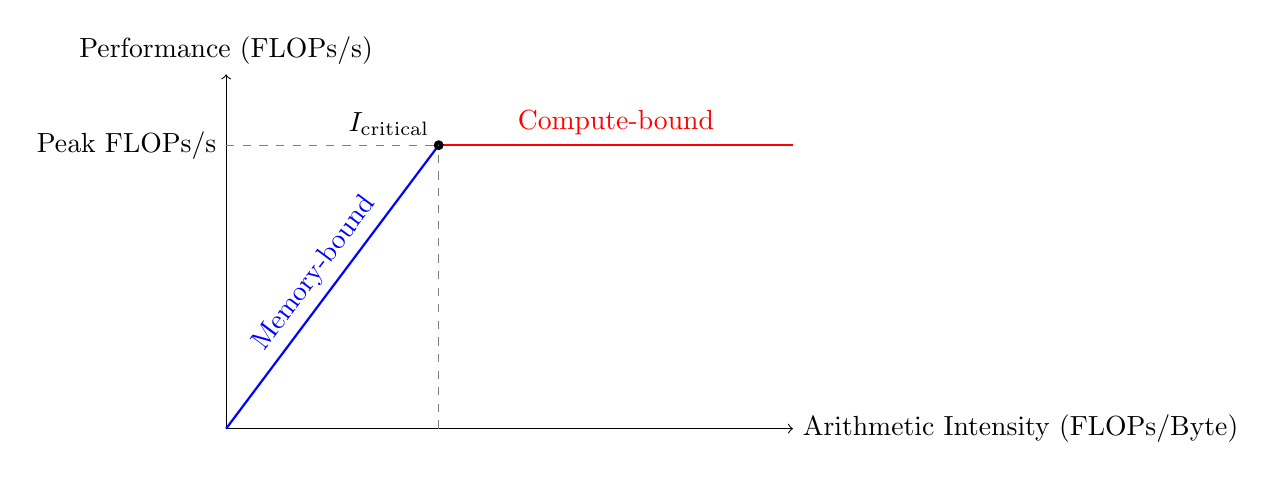
\begin{tikzpicture}[scale=0.9]
        % Axes
        \draw[->] (0,0) -- (8,0) node[right] {Arithmetic Intensity (FLOPs/Byte)};
        \draw[->] (0,0) -- (0,5) node[above] {Performance (FLOPs/s)};

        % Roofline
        \draw[thick, blue] (0,0) -- (3,4) node[midway, above, sloped] {Memory-bound};
        \draw[thick, red] (3,4) -- (8,4) node[midway, above] {Compute-bound};

        % Critical point
        \fill (3,4) circle (2pt) node[above left] {$I_{\text{critical}}$};

        % Peak lines (dashed)
        \draw[dashed, gray] (0,4) -- (3,4);
        \draw[dashed, gray] (3,0) -- (3,4);

        % Labels
        \node[left] at (0,4) {Peak FLOPs/s};
    \end{tikzpicture}
    \caption{Roofline模型示意图:性能受内存带宽和计算能力的双重约束}
    \label{fig:roofline}
\end{figure}

\subsection{Hardware Specifications}

表~\ref{tab:hardware_specs}列出了主流AI加速器的关键规格和临界算术强度。

\begin{table}[htbp]
\centering
\caption{主流AI加速器规格对比}
\label{tab:hardware_specs}
\begin{tabular}{lcccc}
\toprule
Hardware & Peak FLOPs/s (BF16) & HBM Bandwidth & $I_{\text{critical}}$ \\
\midrule
NVIDIA A100 & 312 TFLOPs & 2.0 TB/s & $\sim$156 \\
NVIDIA H100 & 990 TFLOPs & 3.35 TB/s & $\sim$296 \\
Google TPU v5e & 197 TFLOPs & 820 GB/s & $\sim$240 \\
AMD MI300X & 1,307 TFLOPs & 5.3 TB/s & $\sim$247 \\
\bottomrule
\end{tabular}
\end{table}

\subsection{Matrix Multiplication Analysis}

矩阵乘法是Transformer的核心计算。对于 $C = AB$,其中 $A \in \R^{B \times D}$,$B \in \R^{D \times F}$:
\begin{equation}
    \text{FLOPs} = 2BDF
\end{equation}
\begin{equation}
    \text{Bytes} = 2(BD + DF + BF) \quad \text{(以fp16/bf16计)}
\end{equation}
因此算术强度为:
\begin{equation}
    I = \frac{2BDF}{2(BD + DF + BF)} = \frac{BDF}{BD + DF + BF}
\end{equation}
当 $B \ll D, F$ 时(小batch场景),近似为:
\begin{equation}
    I \approx B
\end{equation}

这意味着:
\begin{itemize}
    \item 小batch推理通常是 memory-bound
    \item 增大batch size可以提高计算效率
    \item 对于H100,batch size需要超过$\sim$300才能充分利用计算能力
\end{itemize}

\begin{example}[Transformer推理分析]
考虑一个LLaMA-7B模型在H100上的推理:
\begin{itemize}
    \item 模型维度 $d = 4096$,FFN维度 $d_{ff} = 11008$
    \item 单token推理:$B = 1$,算术强度 $I \approx 1 \ll 296$,严重memory-bound
    \item Batch size = 512:$I \approx 512 > 296$,可以达到compute-bound
\end{itemize}
这解释了为什么大batch推理吞吐量更高。
\end{example}

\subsection{Implications for Transformer Design}

Roofline分析对Transformer的设计和优化有重要指导意义:

\paragraph{注意力机制}
在常见实现中,标准注意力会显式构建大小为 $n \times n$ 的注意力矩阵,并多次读写到HBM,导致HBM访存量随序列长度按 $O(n^2)$ 增长。因此在Roofline模型下,注意力计算是典型的memory-bound kernel。FlashAttention等优化方法通过将计算分块到片上SRAM,避免显式构建 $n^2$ 注意力矩阵并减少HBM读写,从而显著提升性能(详见Section~\ref{sec:flash_attention})。

\paragraph{KV Cache}
自回归生成时,KV cache的加载是主要瓶颈。MQA和GQA通过减少KV头数来降低内存访问量。

\paragraph{模型并行}
当模型过大无法放入单卡时,需要考虑:
\begin{itemize}
    \item \textbf{Tensor Parallelism}: 切分矩阵维度,增加通信但保持计算
    \item \textbf{Pipeline Parallelism}: 切分层,引入bubble但减少通信
    \item \textbf{Expert Parallelism (MoE)}: 专家分布在不同设备,需要all-to-all通信
\end{itemize}

\paragraph{混合精度}
使用INT8权重 + BF16激活时:
\begin{itemize}
    \item 权重加载字节数减半
    \item 算术强度翻倍
    \item 临界batch size降至原来的一半
\end{itemize}

理解这些硬件特性是设计高效Transformer系统的基础。

\subsection{Distributed Training and Sharding}

当模型规模超过单个加速器的内存容量时,需要将参数和计算分布到多个设备上。\textbf{Sharding}(分片)是将张量切分到设备网格上的核心技术。

\begin{definition}[Sharding]
给定一个全局形状为 $[I, J]$ 的张量 $A$ 和一个设备网格 $\mathcal{M}$ 包含轴 $X, Y$,分片记号 $A[I_X, J_Y]$ 表示:
\begin{itemize}
    \item 第一维 $I$ 沿网格轴 $X$ 切分
    \item 第二维 $J$ 沿网格轴 $Y$ 切分
    \item 每个设备持有形状为 $[I/|X|, J/|Y|]$ 的本地分片
\end{itemize}
\end{definition}

\paragraph{分片约束}
一旦某个网格维度被用于切分张量的某个维度,该网格维度就被"消耗",不能再用于同一张量的其他维度。

\subsection{Communication Primitives}

分布式计算中有四个核心通信原语。为便于分析,我们约定:
\begin{itemize}
    \item $V$:每设备本地参与通信的数据量(Bytes)
    \item $N$:参与通信的设备数
    \item $W$:每设备的有效互连带宽(Bytes/s)
    \item $\{U_X\}$:表示沿网格轴 $X$ 的未归约(unreduced)状态
\end{itemize}

\paragraph{AllGather:收集分片}
将分布在各设备的分片收集起来,使每个设备都获得完整数据。
\begin{equation}
    A[I_X, J] \xrightarrow{\text{AllGather}} A[I, J]
\end{equation}
\begin{verbatim}
  之前: D0:[A]    D1:[B]    D2:[C]    D3:[D]      每设备 V
  之后: D0:[ABCD] D1:[ABCD] D2:[ABCD] D3:[ABCD]   每设备 4V
\end{verbatim}
\begin{itemize}
    \item 输入:每设备持有 $V$(全局数据的 $1/N$)
    \item 输出:每设备持有 $N \cdot V$(完整副本)
    \item 通信量:每设备接收 $(N-1) \cdot V$
    \item 成本:$T \approx V/W$(ring算法下,带宽被充分利用)
\end{itemize}

\paragraph{ReduceScatter:归约后分发}
先对各设备数据求和(Reduce),再将结果切分到各设备(Scatter)。
\begin{equation}
    A[I, J]\{U_X\} \xrightarrow{\text{ReduceScatter}} A[I, J_X]
\end{equation}
\begin{verbatim}
  之前: D0:[A0,B0,C0,D0] D1:[A1,B1,C1,D1] D2:[A2,B2,C2,D2] D3:[A3,B3,C3,D3]
        (每设备持有完整但未归约的梯度)
  之后: D0:[ΣA] D1:[ΣB] D2:[ΣC] D3:[ΣD]
        (每设备持有1/4的归约结果,其中 ΣA = A0+A1+A2+A3)
\end{verbatim}
\begin{itemize}
    \item 输入:每设备持有 $V$(未归约,需要与其他设备的对应数据相加)
    \item 输出:每设备持有 $V/N$(归约结果的一个分片)
    \item 成本:$T \approx V/W$
    \item 典型用途:梯度聚合后分片存储(FSDP/ZeRO)
\end{itemize}

\paragraph{AllReduce:归约后广播}
对所有设备的数据求和,并将完整结果发送给每个设备。等价于 ReduceScatter + AllGather。
\begin{equation}
    A[I, J]\{U_X\} \xrightarrow{\text{AllReduce}} A[I, J]
\end{equation}
\begin{verbatim}
  之前: D0:[A0,B0,C0,D0] D1:[A1,B1,C1,D1] D2:[...] D3:[...]  每设备 V
  之后: D0:[ΣA,ΣB,ΣC,ΣD] D1:[ΣA,ΣB,ΣC,ΣD] D2:[...] D3:[...]  每设备 V
        (每设备都持有完整的归约结果)
\end{verbatim}
\begin{itemize}
    \item 输入:每设备持有 $V$(未归约)
    \item 输出:每设备持有 $V$(完整的归约结果)
    \item 成本:$T \approx 2V/W$(两步操作)
    \item 典型用途:DDP梯度同步
\end{itemize}

\paragraph{AllToAll:重新分片}
将数据从一种分片方式转换为另一种,相当于"转置"切分轴。
\begin{equation}
    A[I, J_X] \xrightarrow{\text{AllToAll}} A[I_X, J]
\end{equation}
\begin{verbatim}
  之前: D0:[A0,A1,A2,A3] D1:[B0,B1,B2,B3] D2:[C0,C1,C2,C3] D3:[D0,D1,D2,D3]
        (按"行"切分:每设备持有一整行)
  之后: D0:[A0,B0,C0,D0] D1:[A1,B1,C1,D1] D2:[A2,B2,C2,D2] D3:[A3,B3,C3,D3]
        (按"列"切分:每设备持有一整列)
\end{verbatim}
\begin{itemize}
    \item 输入:每设备持有 $V$(按 $J$ 维切分)
    \item 输出:每设备持有 $V$(按 $I$ 维切分,内容不同但大小相同)
    \item 通信量:每设备发送 $(N-1)/N \cdot V \approx V$,接收同量
    \item 成本:$T \approx V/W$
\end{itemize}

\paragraph{四种通信原语对比}

\begin{table}[htbp]
\centering
\caption{通信原语完整对比($N=4$ 设备,每设备本地数据量 $V$)}
\label{tab:comm_comparison}
\begin{tabular}{lcccc}
\toprule
 & AllGather & ReduceScatter & AllReduce & AllToAll \\
\midrule
数据变化 & 分片$\to$完整 & 完整$\to$分片 & 完整$\to$完整 & 分片$\to$分片 \\
输入大小 & $V$ & $V$ & $V$ & $V$ \\
输出大小 & $N \cdot V$ & $V/N$ & $V$ & $V$ \\
是否归约 & 否 & 是 & 是 & 否 \\
通信成本 & $V/W$ & $V/W$ & $2V/W$ & $V/W$ \\
典型用途 & TP激活收集 & ZeRO梯度分片 & DDP梯度同步 & MoE路由 \\
\bottomrule
\end{tabular}
\end{table}

关键洞察:
\begin{itemize}
    \item \textbf{AllGather}:收集分片,每设备获得相同的完整副本
    \item \textbf{ReduceScatter}:归约后分片,每设备获得不同的归约结果分片
    \item \textbf{AllReduce}:归约后广播,每设备获得相同的完整归约结果(= ReduceScatter + AllGather)
    \item \textbf{AllToAll}:重新分片,每设备获得不同的数据(不归约,仅重分布)
\end{itemize}

\paragraph{AllToAll 在 MoE 中的应用}
MoE(Mixture of Experts)是 AllToAll 的典型应用场景。假设 $N$ 个设备各持有一个 Expert:

\begin{enumerate}
    \item \textbf{Router} 决定每个 token 应由哪个 Expert 处理
    \item \textbf{Dispatch}(AllToAll):将 token 发送到目标 Expert 所在设备
    \item \textbf{Expert 计算}:每设备用本地 Expert 处理收到的 token
    \item \textbf{Combine}(AllToAll):将结果发回原设备
\end{enumerate}

AllToAll 使得 token 能够高效地"找到"分布在不同设备上的 Expert,而无需在每个设备上复制所有 token。

\subsection{Distributed Matrix Multiplication}

分布式矩阵乘法 $C = AB$ 的通信策略取决于输入的分片模式:

\paragraph{Case 1: 非收缩维分片(无通信)}
\begin{equation}
    A[I_X, J] \cdot B[J, K_Y] \to C[I_X, K_Y]
\end{equation}
输出自动继承输入的分片模式,无需通信。

\paragraph{Case 2: 单输入收缩维分片(AllGather)}
\begin{equation}
    A[I, J_X] \cdot B[J, K] \xrightarrow{\text{AllGather}} A[I, J] \cdot B[J, K] \to C[I, K]
\end{equation}
需要先AllGather移除 $A$ 的分片。

\paragraph{Case 3: 双输入同轴收缩维分片(AllReduce)}
\begin{equation}
    A[I, J_X] \cdot B[J_X, K] \to C[I, K]\{U_X\} \xrightarrow{\text{AllReduce}} C[I, K]
\end{equation}
本地矩阵乘法产生部分和,AllReduce完成归约。

\paragraph{Case 4: 双输入同轴非收缩维分片(非法)}
\begin{equation}
    A[I_X, J] \cdot B[J, K_X] \to \text{Invalid (diagonal result)}
\end{equation}
必须先AllGather其中一个输入。

\begin{example}[策略选择]
对于 $C = AB$,其中 $A \in \R^{B \times D}$,$B \in \R^{D \times F}$,比较两种策略:

\textbf{策略1}(AllGather优先):
\begin{equation}
    T_1 = \underbrace{\frac{2DF}{W}}_{\text{AllGather } B} + \underbrace{\frac{2BDF}{C}}_{\text{Compute}}
\end{equation}

\textbf{策略2}(AllReduce优先):
\begin{equation}
    T_2 = \underbrace{\frac{4BF}{W}}_{\text{AllReduce } C} + \underbrace{\frac{2BDF/X}{C}}_{\text{Local Compute}}
\end{equation}

当 $D > 2X$(模型维度远大于并行度)时,策略2更优。
\end{example}

\subsection{Parallelism Strategies}

大规模Transformer训练通常结合多种并行策略:

\paragraph{Data Parallelism (DP)}
将batch维度切分到多个设备,每个设备持有完整模型副本:
\begin{itemize}
    \item 前向传播:各设备独立计算
    \item 反向传播:AllReduce同步梯度
    \item 优点:实现简单,通信量与模型大小成正比
    \item 缺点:内存冗余(每设备存完整模型)
\end{itemize}

\paragraph{Fully Sharded Data Parallelism (FSDP/ZeRO)}
将参数、梯度、优化器状态都沿数据维度切分:
\begin{equation}
    \text{Memory/device} = \frac{\text{Model Size}}{N_{\text{devices}}} + \text{Activations}
\end{equation}
计算前AllGather参数,计算后ReduceScatter梯度。

\paragraph{Tensor Parallelism (TP)}
将矩阵维度切分,每层内部并行计算:
\begin{itemize}
    \item Column Parallel:$W[D, F_X]$,前向AllGather,反向ReduceScatter
    \item Row Parallel:$W[D_X, F]$,前向ReduceScatter,反向AllGather
\end{itemize}
通常在Transformer的Attention和FFN中交替使用,每层需要2次AllReduce。

\paragraph{Pipeline Parallelism (PP)}
将模型层切分到不同设备,形成流水线:
\begin{itemize}
    \item 优点:通信量少(仅传递激活值)
    \item 缺点:存在流水线气泡(bubble),降低硬件利用率
    \item 优化:1F1B调度、交错调度等减少bubble
\end{itemize}

\paragraph{Expert Parallelism (EP)}
MoE模型中,不同专家分布在不同设备:
\begin{equation}
    \text{Input}[B, D] \xrightarrow{\text{AllToAll}} \text{Expert}_i[B_i, D] \xrightarrow{\text{Compute}} \xrightarrow{\text{AllToAll}} \text{Output}[B, D]
\end{equation}
需要AllToAll进行token路由和结果收集。

\paragraph{Sequence Parallelism (SP)}
将序列维度切分,与TP配合使用:
\begin{itemize}
    \item LayerNorm和Dropout沿序列维度切分
    \item 减少激活值内存
    \item 与TP共享通信,无额外开销
\end{itemize}

\subsection{Communication-Computation Overlap}

高效的分布式系统通过重叠通信和计算来隐藏通信延迟:

\begin{equation}
    T_{\text{total}} = \max(T_{\text{compute}}, T_{\text{comm}}) \quad \text{(理想情况)}
\end{equation}

实现技术:
\begin{itemize}
    \item \textbf{异步通信}:在计算进行时启动下一次通信
    \item \textbf{分块流水线}:将大张量切分为小块,交替计算和通信
    \item \textbf{梯度累积}:多个micro-batch累积后再同步
\end{itemize}

理解这些分布式并行技术是扩展Transformer到千亿参数规模的关键。

\newpage\section{Transformer计算分析}
\label{sec:transformer_math}

本节从计算角度系统分析Transformer架构,涵盖FLOPs计算、参数量统计、内存占用,以及推理优化。理解这些数学关系对于模型设计、训练规划和部署优化至关重要。

% ============================================
% 符号定义
% ============================================
\subsection{符号定义}

表~\ref{tab:notation}列出了本节使用的符号。图~\ref{fig:transformer_diagram}展示了Transformer单层的完整计算流程。

\begin{table}[htbp]
\centering
\caption{Transformer计算分析符号表}
\label{tab:notation}
\begin{tabular}{cl}
\toprule
符号 & 含义 \\
\midrule
$B$ & Batch size \\
$T$ & 序列长度(Sequence length) \\
$D$ & 模型维度(Hidden dimension) \\
$F$ & FFN中间维度(通常 $F = 4D$ 或 $\frac{8}{3}D$) \\
$L$ & Transformer层数 \\
$N$ & Query head数量 \\
$K$ & KV head数量(MHA: $K=N$,GQA: $K<N$,MQA: $K=1$) \\
$H$ & 每个head的维度(通常 $H = D/N$) \\
$V$ & 词表大小(Vocabulary size) \\
$P$ & 模型总参数量 \\
\bottomrule
\end{tabular}
\end{table}

\begin{figure}[H]
\centering
\includegraphics[width=0.75\textwidth]{figures/transformer-diagram.png}
\caption{Transformer层的计算流程与张量维度。上:Attention模块;下:MLP模块(SwiGLU)。}
\label{fig:transformer_diagram}
\end{figure}

% ============================================
% 基础运算
% ============================================
\subsection{基础运算}

矩阵运算是Transformer的计算基础。设矩阵维度为 $m, n, k$:

\begin{table}[htbp]
\centering
\caption{基本矩阵运算的FLOPs与数据传输}
\label{tab:basic_ops}
\begin{tabular}{lccc}
\toprule
运算 & 表达式 & FLOPs & 数据量 \\
\midrule
向量点积 & $\bm{x} \cdot \bm{y}$, $\bm{x}, \bm{y} \in \R^k$ & $2k$ & $2k$ \\
矩阵-向量乘 & $A\bm{x}$, $A \in \R^{m \times k}$ & $2mk$ & $mk + k$ \\
矩阵-矩阵乘 & $AB$, $A \in \R^{m \times k}, B \in \R^{k \times n}$ & $2mkn$ & $mk + kn$ \\
\bottomrule
\end{tabular}
\end{table}

\paragraph{前向与反向传播}
对于线性层 $Y = XW$($X \in \R^{m \times k}$,$W \in \R^{k \times n}$):
\begin{itemize}
    \item 前向:$Y = XW$,FLOPs $= 2mkn$
    \item 反向:$\frac{\partial L}{\partial X} = \frac{\partial L}{\partial Y} W^\top$($2mkn$)+ $\frac{\partial L}{\partial W} = X^\top \frac{\partial L}{\partial Y}$($2mkn$)
    \item 总计:$6mkn$ FLOPs
\end{itemize}

这导出了训练FLOPs的核心公式:
\begin{equation}
    \boxed{\text{Training FLOPs} \approx 6 \times P \times T_{\text{tokens}}}
    \label{eq:6nd}
\end{equation}
其中 $P$ 是参数量,$T_{\text{tokens}}$ 是训练token总数。

% ============================================
% 单层分析
% ============================================
\subsection{单层分析}

Transformer每层包含两个核心模块:Attention和MLP。

\subsubsection{MLP层}

MLP层(也称FFN)有两种常见形式:

\paragraph{Standard FFN}
\begin{equation}
    \text{FFN}(x) = W_2 \cdot \text{GELU}(W_1 x), \quad W_1 \in \R^{D \times F}, W_2 \in \R^{F \times D}
\end{equation}

\paragraph{SwiGLU FFN}
\begin{equation}
    \text{SwiGLU}(x) = W_2 \cdot (\text{SiLU}(W_1 x) \odot W_3 x), \quad W_1, W_3 \in \R^{D \times F}, W_2 \in \R^{F \times D}
\end{equation}

其中 $\odot$ 是逐元素乘法,起\textbf{门控}作用:$W_3 x$ 控制 $\text{SiLU}(W_1 x)$ 的信息流通。

\begin{table}[htbp]
\centering
\caption{MLP层参数与FLOPs(per layer, 输入shape $[B, T, D]$)}
\label{tab:mlp_flops}
\begin{tabular}{lccc}
\toprule
类型 & 参数量 & 前向FLOPs & 训练FLOPs \\
\midrule
Standard FFN & $2DF$ & $4BTDF$ & $12BTDF$ \\
SwiGLU & $3DF$ & $6BTDF$ & $18BTDF$ \\
\bottomrule
\end{tabular}
\end{table}

\begin{remark}[参数量一致性]
为保持总参数量一致,不同结构调整 $F$ 的取值:
\begin{itemize}
    \item Standard FFN:$F = 4D$ $\Rightarrow$ 参数量 $= 8D^2$
    \item SwiGLU:$F = \frac{8}{3}D$ $\Rightarrow$ 参数量 $= 8D^2$
\end{itemize}
现代模型(LLaMA、DeepSeek等)普遍采用SwiGLU。
\end{remark}

\subsubsection{Attention层}

Multi-Head Attention包含四个投影和注意力计算:
\begin{align}
    Q = XW_Q, \quad K = XW_K, \quad V = XW_V, \quad O = \text{Attn}(Q, K, V) W_O
\end{align}
其中 $W_Q, W_O \in \R^{D \times D}$,$W_K, W_V \in \R^{D \times KH}$。

\begin{equation}
    \text{Attn}(Q, K, V) = \text{softmax}\left(\frac{QK^\top}{\sqrt{H}}\right)V
\end{equation}

\begin{table}[htbp]
\centering
\caption{Attention层参数与FLOPs(per layer, GQA with $K$ KV heads)}
\label{tab:attn_flops}
\begin{tabular}{lcc}
\toprule
组件 & 参数量 & 训练FLOPs \\
\midrule
Q projection & $D^2$ & $6BTD^2$ \\
K projection & $DKH$ & $6BTDKH$ \\
V projection & $DKH$ & $6BTDKH$ \\
O projection & $D^2$ & $6BTD^2$ \\
$QK^\top$ & — & $6BT^2NH$ \\
$\text{softmax} \cdot V$ & — & $6BT^2NH$ \\
\midrule
\textbf{Total} & $2D^2 + 2DKH$ & $12BTD^2 + 12BTDKH + 12BT^2NH$ \\
\bottomrule
\end{tabular}
\end{table}

\paragraph{MHA / GQA / MQA对比}
\begin{itemize}
    \item \textbf{MHA}(Multi-Head Attention):$K = N$,每个head独立KV
    \item \textbf{GQA}(Grouped-Query Attention):$1 < K < N$,多个Q head共享KV
    \item \textbf{MQA}(Multi-Query Attention):$K = 1$,所有head共享一个KV
\end{itemize}

\subsubsection{Attention vs MLP 计算量对比}

简化假设($F = 4D$,$K \ll N$,$NH = D$)下:
\begin{equation}
    \frac{\text{Attention FLOPs}}{\text{MLP FLOPs}} \approx \frac{T}{8D}
\end{equation}

\begin{remark}
当 $T < 8D$ 时,\textbf{MLP计算量主导}。对于 $D = 8192$ 的模型,序列长度需超过 $65536$ 才能使注意力成为主要计算瓶颈。这解释了为什么长上下文场景才需要特别关注注意力效率。
\end{remark}

% ============================================
% 完整模型分析
% ============================================
\subsection{完整模型分析}

\subsubsection{总参数量}

完整Transformer模型的参数组成:
\begin{flalign}
    & P_{\text{embed}} = VD && \text{(词嵌入)} & \\
    & P_{\text{attn}} = L \cdot (2D^2 + 2DKH) && \text{(注意力层)} & \\
    & P_{\text{mlp}} = L \cdot 3DF && \text{(MLP层,SwiGLU)} & \\
    & P_{\text{norm}} = L \cdot 4D && \text{(LayerNorm)} & \\
    & P_{\text{head}} = DV && \text{(输出投影)} &
\end{flalign}

总参数量(不共享embedding时):
\begin{equation}
    \boxed{P_{\text{total}} = 2VD + L \cdot (2D^2 + 2DKH + 3DF + 4D)}
\end{equation}

\begin{example}[LLaMA-7B参数计算]
$D = 4096$, $F = 11008$, $L = 32$, $V = 32000$, $N = K = 32$(MHA), $H = 128$:
\begin{align}
    P_{\text{embed}} &= 32000 \times 4096 = 131\text{M} \\
    P_{\text{attn/layer}} &= 2 \times 4096^2 + 2 \times 4096 \times 32 \times 128 = 67\text{M} \\
    P_{\text{mlp/layer}} &= 3 \times 4096 \times 11008 = 135\text{M} \\
    P_{\text{total}} &\approx 2 \times 131\text{M} + 32 \times (67\text{M} + 135\text{M}) \approx \mathbf{6.7B}
\end{align}
\end{example}

\subsubsection{训练计算量}

每token的训练FLOPs(忽略注意力中的 $T^2$ 项):
\begin{equation}
    \text{FLOPs/token} \approx 6P + 12LT \cdot NH
\end{equation}

第一项 $6P$ 是参数相关计算(占主导),第二项是注意力的序列长度相关计算。

\begin{table}[htbp]
\centering
\caption{常见模型的计算量}
\label{tab:model_flops}
\begin{tabular}{lccc}
\toprule
模型 & 参数量 & 前向FLOPs/token & 训练FLOPs/token \\
\midrule
GPT-2 & 1.5B & 3B & 9B \\
LLaMA-7B & 6.7B & 13B & 40B \\
LLaMA-70B & 70B & 140B & 420B \\
GPT-4 (est.) & 1.8T & 3.6T & 11T \\
\bottomrule
\end{tabular}
\end{table}

\subsubsection{训练内存占用}

训练时的内存组成:

\begin{table}[htbp]
\centering
\caption{训练内存组成($P$ 为参数量)}
\label{tab:memory}
\begin{tabular}{lcc}
\toprule
组件 & 内存 & 说明 \\
\midrule
参数(bf16) & $2P$ & 模型权重 \\
梯度(bf16) & $2P$ & 反向传播梯度 \\
优化器状态(Adam, fp32) & $8P$ & momentum + variance \\
激活值 & $O(BTD \cdot L)$ & 中间结果,用于反向传播 \\
\midrule
\textbf{总计(无优化)} & $\approx 12P + \text{activations}$ & \\
\bottomrule
\end{tabular}
\end{table}

\paragraph{Activation Checkpointing}
通过只保存每层输入、重新计算中间激活来节省内存:
\begin{itemize}
    \item 内存:从 $O(L \cdot BTD)$ 降至 $O(BTD)$
    \item 代价:额外约33\%重计算($6P \to 8P$)
\end{itemize}

% ============================================
% 推理分析
% ============================================
\subsection{推理分析}

推理与训练有本质区别:无需梯度和优化器状态,但自回归生成引入新的挑战。

\subsubsection{KV Cache}

自回归生成时,每生成一个token需要attend到所有历史token。为避免重复计算,需缓存历史的K和V:
\begin{equation}
    \boxed{\text{KV Cache Size} = 2 \times B \times S \times L \times K \times H \times \text{bytes}}
\end{equation}
其中 $S$ 是当前序列长度,$K$ 是KV head数,$H$ 是head维度。

\begin{example}[KV Cache计算]
70B模型:$D = 8192$, $L = 80$, $K = 8$(GQA), $H = 128$, $S = 8192$, bf16精度:
\begin{equation}
    \text{KV Cache} = 2 \times 1 \times 8192 \times 80 \times 8 \times 128 \times 2 = \mathbf{2.1\text{ GB/request}}
\end{equation}
\end{example}

\paragraph{KV Cache的影响}
\begin{itemize}
    \item 内存瓶颈:限制最大batch size和上下文长度
    \item GQA/MQA:通过减少 $K$ 降低cache大小(如从32降到8,减少4倍)
    \item 量化:int8/int4进一步压缩(2-4倍)
\end{itemize}

\subsubsection{Prefill vs Decode}

推理分为两个阶段,具有不同的计算特性:

\begin{table}[htbp]
\centering
\caption{Prefill vs Decode对比}
\label{tab:prefill_decode_overview}
\begin{tabular}{lcc}
\toprule
 & Prefill & Decode \\
\midrule
输入 & 整个prompt($T$ tokens) & 单个token \\
计算模式 & 并行处理所有token & 逐token生成 \\
瓶颈 & Compute-bound & Memory-bound \\
主要开销 & 矩阵乘法计算 & 权重加载 + KV Cache读写 \\
优化方向 & 提高计算利用率 & 增大batch、减少访存 \\
\bottomrule
\end{tabular}
\end{table}

\subsubsection{推理优化策略}

\paragraph{Batching策略}
\begin{itemize}
    \item \textbf{Continuous Batching}:动态插入/移除请求,提高GPU利用率
    \item \textbf{Chunked Prefill}:将长prompt分块处理,与decode交错执行
\end{itemize}

\paragraph{投机解码(Speculative Decoding)}
用小模型快速生成候选token序列,大模型并行验证:
\begin{itemize}
    \item 小模型(draft):快速生成 $k$ 个候选token
    \item 大模型(verify):一次前向验证所有候选,接受正确的前缀
    \item 加速比:$1.5\times \sim 3\times$(取决于draft模型准确率)
\end{itemize}

\paragraph{量化}
\begin{itemize}
    \item \textbf{Weight-only}(W4A16):权重int4,激活fp16,减少权重加载
    \item \textbf{Full quantization}(W8A8):权重和激活都int8,利用INT8 Tensor Core
\end{itemize}

\newpage\section{Scaling Law}
\label{sec:scaling_law}

Scaling Law(缩放定律)揭示了大语言模型性能与计算量、数据量、模型规模之间的幂律关系,是指导LLM训练资源分配的核心理论。

\subsection{基本概念}

\subsubsection{什么是Scaling Law}

Scaling Law描述了模型性能(通常用损失函数$L$衡量)如何随资源增加而改善:
\begin{equation}
    L = \left(\frac{N_c}{N}\right)^{\alpha_N} + \left(\frac{D_c}{D}\right)^{\alpha_D} + L_\infty
\end{equation}
其中:
\begin{itemize}
    \item $N$:模型参数量
    \item $D$:训练数据量(tokens)
    \item $L_\infty$:不可约损失(数据本身的熵)
    \item $N_c, D_c, \alpha_N, \alpha_D$:拟合常数
\end{itemize}

\subsubsection{为什么Scaling Law重要}

\begin{itemize}
    \item \textbf{资源分配}:给定计算预算,如何分配模型大小和数据量
    \item \textbf{性能预测}:在小规模实验预测大规模模型的性能
    \item \textbf{投资决策}:估算达到目标性能所需的资源
\end{itemize}

\subsection{Kaplan Scaling Law (2020)}

OpenAI的Kaplan等人~\citep{kaplan2020scaling}首次系统研究了LLM的Scaling Law。

\subsubsection{核心发现}

\paragraph{性能与规模的幂律关系}
\begin{align}
    L(N) &= \left(\frac{N_c}{N}\right)^{\alpha_N}, \quad \alpha_N \approx 0.076 \\
    L(D) &= \left(\frac{D_c}{D}\right)^{\alpha_D}, \quad \alpha_D \approx 0.095 \\
    L(C) &= \left(\frac{C_c}{C}\right)^{\alpha_C}, \quad \alpha_C \approx 0.050
\end{align}
其中$C$是计算量(FLOPs)。

\paragraph{关键结论}
\begin{enumerate}
    \item \textbf{模型规模主导}:在固定计算预算下,更大的模型(训练更少步数)比小模型(训练更多步数)更优
    \item \textbf{最优分配}:计算量增加10倍时,模型参数应增加约5.5倍,数据量增加约1.8倍
    \item \textbf{架构不敏感}:Scaling Law对Transformer的具体超参数(层数、宽度)不敏感
\end{enumerate}

\subsubsection{计算最优模型}

Kaplan建议的计算最优分配:
\begin{equation}
    N_{opt} \propto C^{0.73}, \quad D_{opt} \propto C^{0.27}
\end{equation}

这意味着随着计算预算增加,应该更多地投资于模型规模而非数据量。

\subsection{Chinchilla Scaling Law (2022)}

DeepMind的Hoffmann等人~\citep{hoffmann2022chinchilla}挑战了Kaplan的结论,提出了更均衡的分配策略。

\subsubsection{核心发现}

\paragraph{数据的重要性被低估}
Chinchilla研究表明,之前的模型普遍欠拟合(undertrained):
\begin{itemize}
    \item GPT-3 (175B):训练了300B tokens,但最优应该是约3.5T tokens
    \item Gopher (280B):训练了300B tokens,同样严重不足
\end{itemize}

\paragraph{新的最优分配}
\begin{equation}
    N_{opt} \propto C^{0.50}, \quad D_{opt} \propto C^{0.50}
\end{equation}

更简洁的表述:
\begin{equation}
    D_{opt} \approx 20 \times N
    \label{eq:chinchilla}
\end{equation}

即\textbf{最优训练数据量约为模型参数的20倍}。

\subsubsection{为什么是20倍?推导直觉}

这个看似任意的常数背后有清晰的数学逻辑。考虑计算预算约束 $C = 6ND$(FLOPs $\approx$ 6 × 参数 × tokens),目标是最小化损失:

\begin{equation}
    L(N, D) = \frac{A}{N^{\alpha}} + \frac{B}{D^{\beta}} + L_\infty
\end{equation}

在约束 $C = 6ND$ 下求极值,使用拉格朗日乘数法:
\begin{equation}
    \frac{\partial L}{\partial N} \bigg/ \frac{\partial L}{\partial D} = \frac{D}{N}
\end{equation}

代入幂律形式:
\begin{equation}
    \frac{\alpha A / N^{\alpha+1}}{\beta B / D^{\beta+1}} = \frac{D}{N} \implies \frac{D}{N} = \left(\frac{\alpha A}{\beta B}\right)^{\frac{1}{\alpha+\beta+2}}
\end{equation}

Chinchilla的实验测得 $\alpha \approx 0.34$,$\beta \approx 0.28$,代入后得到 $D/N \approx 20$。

\paragraph{物理直觉}
这个结果可以这样理解:模型参数需要足够的"训练信号"才能收敛到最优值。每个参数平均需要看到约20个tokens的信息才能学到有意义的表示。参数太多(相对于数据)会欠拟合——模型有容量但缺乏信号;数据太多(相对于参数)会浪费——模型容量已饱和,额外数据无法被利用。

\paragraph{Kaplan vs Chinchilla:争议的本质}
两个团队得出不同结论的根本原因在于\textbf{实验设计}:
\begin{itemize}
    \item Kaplan固定训练步数,变化模型大小——这倾向于发现"大模型更好"
    \item Chinchilla固定计算量,同时变化模型和数据——这才能找到真正的帕累托最优
\end{itemize}

Chinchilla的设计更接近实际资源分配问题:给定固定预算,如何分配?

\subsubsection{Chinchilla模型验证}

DeepMind训练了70B参数的Chinchilla模型,使用1.4T tokens:
\begin{itemize}
    \item 计算量与Gopher (280B)相同
    \item 性能全面超越Gopher
    \item 推理成本降低4倍(参数量是1/4)
\end{itemize}

\begin{table}[htbp]
\centering
\caption{Chinchilla vs Gopher性能对比}
\label{tab:chinchilla_vs_gopher}
\begin{tabular}{lccc}
\toprule
模型 & 参数量 & 训练Tokens & MMLU \\
\midrule
Gopher & 280B & 300B & 60.0\% \\
Chinchilla & 70B & 1.4T & 67.6\% \\
\bottomrule
\end{tabular}
\end{table}

\subsubsection{对工业界的影响}

Chinchilla Law深刻影响了后续模型的设计:

\begin{table}[htbp]
\centering
\caption{主流模型的参数-数据配比}
\label{tab:model_data_ratio}
\begin{tabular}{lccc}
\toprule
模型 & 参数量 & 训练Tokens & Tokens/参数 \\
\midrule
GPT-3 & 175B & 300B & 1.7$\times$ \\
Chinchilla & 70B & 1.4T & 20$\times$ \\
LLaMA & 65B & 1.4T & 21.5$\times$ \\
LLaMA 2 & 70B & 2T & 28.6$\times$ \\
LLaMA 3 & 70B & 15T & 214$\times$ \\
Qwen 2 & 72B & 7T+ & 97$\times$ \\
\bottomrule
\end{tabular}
\end{table}

\subsection{超越Chinchilla:推理最优的视角}

Chinchilla法则解决的是"训练最优"问题:给定计算预算,如何最小化训练后的损失?但在工业部署中,问题的形式不同:给定\textbf{总预算}(训练+推理),如何最大化用户价值?

\subsubsection{训练-推理权衡的数学框架}

设总成本为训练成本加上生命周期内的推理成本:
\begin{equation}
    \text{Total Cost} = C_{train} + n_{infer} \times C_{infer}(N)
\end{equation}

其中 $C_{train} = 6ND$,$C_{infer}(N) \propto N$(推理成本与参数量成正比)。

\paragraph{关键洞察}
Chinchilla最优假设 $n_{infer} = 0$——只考虑训练。但当 $n_{infer}$ 很大时,推理成本主导总成本。此时最优策略发生根本转变:
\begin{itemize}
    \item \textbf{小模型}:$C_{infer}$ 低,即使每个query成本微小,累积量也可观
    \item \textbf{Over-training}:用额外训练成本换取更小模型的性能,摊薄到海量推理中
\end{itemize}

\paragraph{定量分析}
假设目标性能固定,两种策略的成本对比:
\begin{enumerate}
    \item Chinchilla最优:70B模型 + 1.4T tokens,$C_{train} \propto 70 \times 1.4 = 98$
    \item Over-training:8B模型 + 15T tokens,$C_{train} \propto 8 \times 15 = 120$
\end{enumerate}

训练成本增加22\%,但推理成本降低88\%($8/70$)。当 $n_{infer} > 10^9$ 时(对于ChatGPT级产品很常见),Over-training策略的总成本显著更低。

\subsubsection{LLaMA的策略}

LLaMA系列采用激进的Over-training:
\begin{itemize}
    \item LLaMA-7B:1T tokens(143$\times$参数)
    \item LLaMA 2-7B:2T tokens(286$\times$参数)
    \item LLaMA 3-8B:15T tokens(1875$\times$参数)
\end{itemize}

\begin{remark}[Over-training的收益递减]
虽然Over-training有益,但收益递减:
\begin{itemize}
    \item 早期:每增加1倍数据,性能显著提升
    \item 后期:需要更多数据才能获得同样提升
    \item 存在实际上限:数据重复使用最终会导致过拟合
\end{itemize}
\end{remark}

\subsection{多维度Scaling Law}

\subsubsection{下游任务Scaling}

预训练Loss的Scaling Law不完全转化为下游任务性能:

\begin{itemize}
    \item \textbf{涌现能力}:某些能力在特定规模突然出现
    \item \textbf{任务依赖}:不同任务的Scaling曲线不同
    \item \textbf{评估敏感}:度量方式影响观察到的Scaling行为
\end{itemize}

\subsubsection{RLHF/DPO的Scaling}

后训练也遵循Scaling Law,但形式不同:

\begin{itemize}
    \item \textbf{基座模型规模}:更大的基座模型对齐效果更好
    \item \textbf{偏好数据量}:收益递减明显,质量比数量重要
    \item \textbf{Reward Model}:RM规模通常应与Policy规模匹配
\end{itemize}

\subsubsection{推理时Scaling(Test-time Compute)}

OpenAI o1等推理模型展示了新的Scaling维度:

\begin{equation}
    \text{Performance} = f(\text{Pretraining Compute}, \text{Inference Compute})
\end{equation}

\begin{itemize}
    \item 通过更多推理时计算(更长的思考链)提升性能
    \item 与预训练计算形成互补
    \item 开辟了``用推理换性能''的新范式
\end{itemize}

\subsection{Scaling Law的局限与争议}

\subsubsection{局限性}

\begin{itemize}
    \item \textbf{外推风险}:从小规模实验外推大规模可能失准
    \item \textbf{数据质量}:Scaling Law假设数据质量恒定
    \item \textbf{架构依赖}:不同架构可能有不同的Scaling行为
    \item \textbf{任务特定}:通用Scaling Law可能不适用于特定任务
\end{itemize}

\subsubsection{数据墙(Data Wall)}

\paragraph{高质量数据枯竭}
\begin{itemize}
    \item 互联网高质量文本有限(估计约10-15T tokens)
    \item 继续Scaling需要合成数据或其他来源
    \item 数据重复使用有上限
\end{itemize}

\paragraph{应对策略}
\begin{itemize}
    \item \textbf{合成数据}:用模型生成训练数据
    \item \textbf{数据增强}:改写、翻译、多样化
    \item \textbf{多模态数据}:图像、视频、音频
    \item \textbf{代码数据}:GitHub等代码仓库
\end{itemize}

\subsubsection{涌现能力的争议}

\paragraph{涌现是真实的吗?}
有研究认为``涌现能力''可能是评估度量的假象:
\begin{itemize}
    \item 使用连续度量(如token-level准确率)替代离散度量
    \item 重新分析后,很多``涌现''变成平滑的Scaling
\end{itemize}

\paragraph{实践意义}
无论涌现是否真实存在,大模型确实展现出小模型没有的能力,这对应用仍然重要。

\subsection{Scaling Law的实践应用}

\subsubsection{预测模型性能}

利用Scaling Law进行性能预测:
\begin{enumerate}
    \item 训练多个小规模模型(不同大小、不同数据量)
    \item 拟合Scaling Law参数
    \item 外推预测大规模模型性能
    \item 决定是否值得投资大规模训练
\end{enumerate}

\subsubsection{资源分配决策}

给定计算预算$C$,如何分配:

\paragraph{训练最优(Chinchilla)}
\begin{align}
    N &= \sqrt{C / 6D} \\
    D &= 20N
\end{align}

\paragraph{推理最优}
根据预期推理量$n_{infer}$调整:
\begin{itemize}
    \item $n_{infer}$小:接近Chinchilla最优
    \item $n_{infer}$大:Over-train更小的模型
\end{itemize}

\subsubsection{Scaling Law拟合示例}

\begin{lstlisting}
import numpy as np
from scipy.optimize import curve_fit

def scaling_law(x, a, b, c):
    """L = a / x^b + c"""
    return a / np.power(x, b) + c

# 实验数据:(参数量, 损失)
params = [125e6, 350e6, 760e6, 1.3e9, 2.7e9, 6.7e9]
losses = [3.50, 3.25, 3.10, 2.95, 2.80, 2.65]

# 拟合
popt, _ = curve_fit(scaling_law, params, losses)
a, b, c = popt

# 预测70B模型的损失
pred_loss = scaling_law(70e9, a, b, c)
print(f"Predicted loss for 70B: {pred_loss:.2f}")
\end{lstlisting}

\begin{remark}[Scaling Law使用建议]
\begin{itemize}
    \item \textbf{小规模验证}:在投入大规模训练前,用小模型验证假设
    \item \textbf{多点拟合}:至少3-5个不同规模的数据点
    \item \textbf{保守外推}:外推倍数不宜过大(通常$<$10倍)
    \item \textbf{任务相关}:关注目标任务的Scaling,而非只看Loss
    \item \textbf{持续监控}:大规模训练时监控是否符合预期
\end{itemize}
\end{remark}


% ============================================
% Part II: Transformer核心组件
% ============================================
\newpage
\part{Transformer核心组件}
\newpage\section{分词器(Tokenizer)}
\label{sec:tokenizer}

分词器是大语言模型的入口,负责将原始文本转换为模型可处理的token序列。分词策略的选择直接影响模型的词表大小、训练效率和多语言能力。

\subsection{为什么需要分词}

神经网络无法直接处理文本,需要将文本转换为数值表示:
\begin{equation}
    \text{``Hello world''} \xrightarrow{\text{Tokenizer}} [15496, 995] \xrightarrow{\text{Embedding}} \R^{2 \times d}
\end{equation}

分词粒度的选择面临\textbf{词表大小}与\textbf{序列长度}的权衡:

\begin{table}[htbp]
\centering
\caption{不同分词粒度的对比}
\label{tab:tokenization_granularity}
\begin{tabular}{lccc}
\toprule
粒度 & 词表大小 & 序列长度 & 问题 \\
\midrule
字符级 & $\sim$256 & 很长 & 序列过长,难以建模长距离依赖 \\
词级 & $\sim$100K+ & 短 & OOV问题,词表过大 \\
子词级 & $\sim$32K-128K & 适中 & 平衡,主流选择 \\
\bottomrule
\end{tabular}
\end{table}

\subsection{子词分词算法}

\subsubsection{Byte Pair Encoding (BPE)}

BPE~\citep{sennrich2016bpe}是最广泛使用的子词分词算法,源自数据压缩领域。

\paragraph{训练算法}
\begin{enumerate}
    \item 初始化词表为所有字符(或字节)
    \item 统计相邻token对的频率
    \item 将最高频的token对合并为新token,加入词表
    \item 重复步骤2-3,直到达到目标词表大小
\end{enumerate}

\begin{example}[BPE训练过程]
假设语料为:``low lower lowest''
\begin{enumerate}
    \item 初始:\texttt{l, o, w, e, r, s, t, \_}(\_表示词边界)
    \item 最高频对 \texttt{(l, o)} $\to$ 合并为 \texttt{lo}
    \item 最高频对 \texttt{(lo, w)} $\to$ 合并为 \texttt{low}
    \item 最高频对 \texttt{(low, e)} $\to$ 合并为 \texttt{lowe}
    \item ...
\end{enumerate}
最终词表包含常见子词如 \texttt{low}, \texttt{er}, \texttt{est} 等。
\end{example}

\paragraph{分词算法}
给定训练好的合并规则,按优先级依次应用:
\begin{lstlisting}
def bpe_tokenize(text, merges):
    tokens = list(text)  # 初始为字符
    for (a, b) in merges:  # 按训练顺序
        i = 0
        while i < len(tokens) - 1:
            if tokens[i] == a and tokens[i+1] == b:
                tokens = tokens[:i] + [a+b] + tokens[i+2:]
            else:
                i += 1
    return tokens
\end{lstlisting}

\subsubsection{Byte-level BPE}

GPT-2~\citep{radford2019language}引入的改进,直接在字节级别操作:
\begin{itemize}
    \item 基础词表为256个字节,无需预分词
    \item 可以表示任何UTF-8文本,无OOV问题
    \item 避免了不同语言的特殊处理
\end{itemize}

\begin{lstlisting}
# GPT-2的字节到Unicode映射
def bytes_to_unicode():
    # 将256个字节映射到可打印Unicode字符
    # 避免空白字符等控制字符的问题
    bs = list(range(33, 127)) + list(range(161, 173)) + list(range(174, 256))
    cs = bs[:]
    n = 0
    for b in range(256):
        if b not in bs:
            bs.append(b)
            cs.append(256 + n)
            n += 1
    return dict(zip(bs, [chr(c) for c in cs]))
\end{lstlisting}

\subsubsection{WordPiece}

WordPiece由Google提出,用于BERT~\citep{devlin2019bert}。与BPE的主要区别在于合并策略:

\begin{itemize}
    \item \textbf{BPE}:选择频率最高的token对
    \item \textbf{WordPiece}:选择使语言模型似然提升最大的token对
\end{itemize}

WordPiece的合并分数:
\begin{equation}
    \text{score}(a, b) = \frac{\text{freq}(ab)}{\text{freq}(a) \times \text{freq}(b)}
\end{equation}

WordPiece使用 \texttt{\#\#} 标记非词首子词:
\begin{verbatim}
"tokenization" -> ["token", "##ization"]
\end{verbatim}

\subsubsection{Unigram Language Model}

Unigram~\citep{kudo2018sentencepiece}采用相反的策略——从大词表开始,逐步删减:

\begin{enumerate}
    \item 初始化一个较大的候选词表
    \item 用EM算法估计每个token的概率
    \item 计算移除每个token对似然的影响
    \item 移除影响最小的token
    \item 重复直到达到目标词表大小
\end{enumerate}

Unigram的优势:
\begin{itemize}
    \item 同一文本可能有多种分词方式,支持采样
    \item 可用于数据增强(Subword Regularization)
\end{itemize}

\subsection{SentencePiece}

SentencePiece~\citep{kudo2018sentencepiece}是Google开源的分词工具,特点:

\begin{itemize}
    \item \textbf{语言无关}:将空格视为普通字符(用\_表示),无需预分词
    \item \textbf{支持多种算法}:BPE和Unigram
    \item \textbf{可逆}:分词结果可以无损还原原文
    \item \textbf{高效}:C++实现,训练和推理都很快
\end{itemize}

\begin{lstlisting}
import sentencepiece as spm

# 训练
spm.SentencePieceTrainer.train(
    input='corpus.txt',
    model_prefix='tokenizer',
    vocab_size=32000,
    model_type='bpe',  # 或 'unigram'
    character_coverage=0.9995,
)

# 使用
sp = spm.SentencePieceProcessor(model_file='tokenizer.model')
tokens = sp.encode('Hello world', out_type=str)
# ['▁Hello', '▁world']  (▁表示空格)
\end{lstlisting}

\subsection{Tiktoken}

Tiktoken是OpenAI开源的快速BPE实现,用于GPT-3.5/4:

\begin{itemize}
    \item \textbf{Rust实现}:比Python实现快3-6倍
    \item \textbf{正则预分词}:用正则表达式预先切分,提高效率
    \item \textbf{特殊token处理}:支持\texttt{<|endoftext|>}等特殊标记
\end{itemize}

\begin{lstlisting}
import tiktoken

# GPT-4使用cl100k_base编码
enc = tiktoken.get_encoding("cl100k_base")
tokens = enc.encode("Hello world")  # [9906, 1917]
text = enc.decode(tokens)  # "Hello world"

# 查看词表大小
print(enc.n_vocab)  # 100277
\end{lstlisting}

\paragraph{预分词正则}
Tiktoken使用复杂的正则表达式预切分文本:
\begin{lstlisting}
# cl100k_base的预分词正则(简化)
pat = r"""'s|'t|'re|'ve|'m|'ll|'d|
    [\p{L}]+|[\p{N}]{1,3}|
    [^\s\p{L}\p{N}]+|\s+(?!\S)|\s+"""
\end{lstlisting}

这确保了常见模式(如缩写、数字)被合理切分。

\subsection{词表大小的选择}

词表大小是重要的设计决策:

\begin{table}[htbp]
\centering
\caption{主流模型的词表配置}
\label{tab:vocab_sizes}
\begin{tabular}{lcc}
\toprule
模型 & 词表大小 & 分词器 \\
\midrule
GPT-2 & 50,257 & Byte-level BPE \\
GPT-3/3.5 & 50,257 & Byte-level BPE \\
GPT-4 & 100,277 & Byte-level BPE (cl100k) \\
BERT & 30,522 & WordPiece \\
LLaMA & 32,000 & SentencePiece BPE \\
LLaMA 2 & 32,000 & SentencePiece BPE \\
LLaMA 3 & 128,256 & Tiktoken BPE \\
Qwen & 151,936 & Byte-level BPE \\
DeepSeek & 102,400 & Byte-level BPE \\
\bottomrule
\end{tabular}
\end{table}

\paragraph{词表大小的影响}
\begin{itemize}
    \item \textbf{更大词表}:
    \begin{itemize}
        \item 更短的序列长度(同样文本用更少token)
        \item 更大的Embedding层参数($V \times d$)
        \item 更好的多语言支持
    \end{itemize}
    \item \textbf{更小词表}:
    \begin{itemize}
        \item 更长的序列(需要更多token表示)
        \item 更小的模型参数
        \item 稀有词可能被过度切分
    \end{itemize}
\end{itemize}

\paragraph{经验法则}
\begin{itemize}
    \item 英文为主:32K-50K通常足够
    \item 多语言:100K+可以更好覆盖非英语语言
    \item LLaMA 3将词表从32K扩展到128K,中文token效率提升约3倍
\end{itemize}

\subsection{特殊Token}

特殊token用于标记序列结构和控制生成:

\begin{table}[htbp]
\centering
\caption{常见特殊Token}
\label{tab:special_tokens}
\begin{tabular}{lll}
\toprule
Token & 含义 & 用途 \\
\midrule
\texttt{<|endoftext|>} & 文本结束 & 分隔文档,标记生成结束 \\
\texttt{<|im\_start|>} & 消息开始 & ChatML格式的消息边界 \\
\texttt{<|im\_end|>} & 消息结束 & ChatML格式的消息边界 \\
\texttt{[PAD]} & 填充 & 批处理时对齐序列长度 \\
\texttt{[CLS]} & 分类 & BERT的序列表示 \\
\texttt{[SEP]} & 分隔 & BERT的句子分隔 \\
\texttt{[MASK]} & 掩码 & BERT的MLM任务 \\
\bottomrule
\end{tabular}
\end{table}

\paragraph{ChatML格式}
现代Chat模型使用结构化格式区分角色:
\begin{verbatim}
<|im_start|>system
You are a helpful assistant.
<|im_end|>
<|im_start|>user
Hello!
<|im_end|>
<|im_start|>assistant
Hi there!
<|im_end|>
\end{verbatim}

\subsection{多语言分词:一个被低估的公平性问题}

分词器的设计深刻影响着不同语言用户的使用体验。这不仅是技术问题,更是公平性问题。

\subsubsection{Token效率差异的根源}

不同语言的token效率差异显著:

\begin{table}[htbp]
\centering
\caption{不同语言的Token效率(GPT-4,相同语义内容)}
\label{tab:token_efficiency}
\begin{tabular}{lcc}
\toprule
语言 & Token数 & 相对英语 \\
\midrule
英语 & 100 & 1.0$\times$ \\
西班牙语 & 120 & 1.2$\times$ \\
中文 & 150 & 1.5$\times$ \\
日语 & 180 & 1.8$\times$ \\
缅甸语 & 400 & 4.0$\times$ \\
\bottomrule
\end{tabular}
\end{table}

\paragraph{语言学解释}
效率差异源于\textbf{书写系统}与\textbf{训练数据}的双重因素:

\begin{enumerate}
    \item \textbf{字母文字 vs 表意文字}:英语26个字母组合成词,BPE容易学到常见子词(如 \texttt{-tion}, \texttt{-ing})。中文每个字是独立语素,约需3500个常用字覆盖99.9\%文本,但BPE难以学到跨字的有意义组合。

    \item \textbf{训练数据偏斜}:BPE按频率合并token对。当训练语料中英文占90\%时,英文子词被充分合并(\texttt{the}, \texttt{and}成为单token),而中文词汇因频率低而保持拆分状态。

    \item \textbf{UTF-8编码开销}:英文字符占1字节,中文字符占3字节。在Byte-level BPE中,一个中文字至少需要3个基础token才能表示,除非被合并。
\end{enumerate}

\paragraph{定量分析}
设语言$L$在训练语料中的占比为$p_L$,其token效率大致满足:
\begin{equation}
    \text{效率}_L \propto p_L^{\alpha}, \quad \alpha \approx 0.3\text{--}0.5
\end{equation}
这解释了为什么缅甸语(训练数据中几乎没有)效率是英语的1/4——缅甸文字几乎没有被合并,每个字符都被拆成多个字节token。

\subsubsection{实际影响}

对非英语用户而言:
\begin{itemize}
    \item \textbf{成本}:相同语义内容消耗1.5-4倍token,API费用相应增加
    \item \textbf{上下文}:有效上下文窗口缩短(128K tokens对中文用户相当于英文用户的85K)
    \item \textbf{延迟}:生成相同内容需要更多解码步骤
    \item \textbf{质量}:过度切分破坏词汇边界,可能影响语义理解
\end{itemize}

\subsubsection{改进策略}

\paragraph{扩大词表}
LLaMA 3将词表从32K扩展到128K,新增大量非英语token。效果:中文token效率提升约3倍。代价:Embedding层参数增加4倍(从32K$\times d$到128K$\times d$)。

\paragraph{平衡训练语料}
在分词器训练时对语言进行上采样,使低资源语言获得更多合并机会。但这会牺牲高资源语言的效率——存在帕累托权衡。

\paragraph{语言感知分词}
对特定语言使用专门的预分词规则。例如,中文按字切分后再BPE,避免跨字合并产生无意义token。日语可以利用形态分析工具(如MeCab)进行预切分。

\begin{remark}[公平性视角]
分词效率差异本质上是训练资源分配的结果。当商业模型按token计费时,这种差异直接转化为经济不平等——使用小语种的用户为相同服务付出更高代价。这是AI公平性讨论中容易被忽视的技术细节。
\end{remark}

\subsection{分词器的实现细节}

\subsubsection{Tokenizer的组成}

一个完整的分词器包含:
\begin{enumerate}
    \item \textbf{Normalizer}:文本标准化(Unicode归一化、大小写等)
    \item \textbf{Pre-tokenizer}:预分词(按空格、标点切分)
    \item \textbf{Model}:核心分词算法(BPE/WordPiece/Unigram)
    \item \textbf{Post-processor}:后处理(添加特殊token)
    \item \textbf{Decoder}:将token ID还原为文本
\end{enumerate}

\subsubsection{HuggingFace Tokenizers}

HuggingFace的\texttt{tokenizers}库提供高效实现:
\begin{lstlisting}
from tokenizers import Tokenizer, models, trainers, pre_tokenizers

# 创建BPE分词器
tokenizer = Tokenizer(models.BPE())
tokenizer.pre_tokenizer = pre_tokenizers.ByteLevel()

# 训练
trainer = trainers.BpeTrainer(vocab_size=32000, special_tokens=["<|endoftext|>"])
tokenizer.train(files=["corpus.txt"], trainer=trainer)

# 使用
output = tokenizer.encode("Hello world")
print(output.tokens)  # ['Hello', 'Ġworld']
\end{lstlisting}

\subsection{分词的计算开销}

分词通常不是瓶颈,但在某些场景需要注意:

\begin{itemize}
    \item \textbf{在线推理}:分词延迟约0.1-1ms,通常可忽略
    \item \textbf{大规模预处理}:TB级语料分词可能需要数小时
    \item \textbf{优化方法}:
    \begin{itemize}
        \item 使用Rust/C++实现(如Tiktoken)
        \item 并行处理
        \item 预分词缓存
    \end{itemize}
\end{itemize}

\begin{remark}[分词器选择建议]
\begin{itemize}
    \item \textbf{从头训练LLM}:使用SentencePiece或HuggingFace Tokenizers训练专用分词器
    \item \textbf{微调现有模型}:使用原模型的分词器,保持一致性
    \item \textbf{多语言场景}:选择词表较大(100K+)的分词器
    \item \textbf{特殊领域}(代码、数学):考虑在分词器训练时包含领域数据
\end{itemize}
\end{remark}

\newpage\section{位置编码}
\label{sec:position_encoding}

不同于RNN、CNN等模型,Transformer的自注意力机制本身是\textbf{置换不变的}(permutation invariant)——纯粹的Attention模块无法捕捉输入顺序,即无法区分不同位置的Token。为此,位置编码的引入是必不可少的。

位置编码大体有两种思路:
\begin{enumerate}
    \item \textbf{绝对位置编码}:将位置信息融入到输入中,即 $\bm{x}'_k = \bm{x}_k + \bm{p}_k$ 或 $\bm{x}'_k = \bm{x}_k \odot \bm{p}_k$
    \item \textbf{相对位置编码}:微调Attention结构,使其能分辨不同位置的Token
\end{enumerate}

\begin{table}[htbp]
\centering
\caption{位置编码方法分类与对比}
\label{tab:pos_encoding_comparison}
\begin{tabular}{llccl}
\toprule
类型 & 方法 & 作用位置 & 外推性 & 代表模型 \\
\midrule
\multirow{3}{*}{绝对} & Sinusoidal & Embedding & 差 & Transformer \\
 & Learned & Embedding & 差 & BERT, GPT \\
 & FLOATER & Embedding & 中 & — \\
\midrule
\multirow{4}{*}{相对} & 经典式 & Attention & 中 & NEZHA \\
 & T5 Bias & Attention score & 好 & T5 \\
 & ALiBi & Attention score & 好 & BLOOM, MPT \\
 & \textbf{RoPE} & Q/K向量 & 好 & LLaMA, Qwen \\
\bottomrule
\end{tabular}
\end{table}

\subsection{绝对位置编码}

绝对位置编码的一般形式是在输入的第 $k$ 个向量 $\bm{x}_k$ 中加入位置向量 $\bm{p}_k$,其中 $\bm{p}_k$ 只依赖于位置编号 $k$。

\subsubsection{训练式(Learned)}

最朴素的方案是将位置编码作为可训练参数。例如最大长度512、编码维度768,则初始化一个 $512 \times 768$ 的矩阵,随训练更新。BERT、GPT等模型采用此方案。

\paragraph{优点} 简单直接,让模型自己学习位置表示。

\paragraph{缺点} 缺乏外推性——如果预训练最大长度为512,则无法处理更长的序列。虽然可以将超长位置随机初始化后继续微调,但效果有限。

\subsubsection{三角函数式(Sinusoidal)}

原始Transformer~\citep{vaswani2017attention}采用正弦余弦函数生成位置编码:
\begin{align}
    p_{k,2i} &= \sin\left(k / 10000^{2i/d}\right) \\
    p_{k,2i+1} &= \cos\left(k / 10000^{2i/d}\right)
\end{align}
其中 $p_{k,2i}, p_{k,2i+1}$ 分别是位置 $k$ 的编码向量的第 $2i, 2i+1$ 个分量。

\paragraph{设计直觉}
不同维度对应不同频率的周期函数:低维变化快(捕捉局部位置),高维变化慢(捕捉全局位置)。由三角恒等式 $\sin(\alpha+\beta) = \sin\alpha\cos\beta + \cos\alpha\sin\beta$,位置 $\alpha+\beta$ 的向量可表示为位置 $\alpha$ 和 $\beta$ 的向量组合,这提供了表达相对位置信息的可能性。

\paragraph{局限性}
尽管有显式的生成规律,但实践中Sinusoidal编码的外推能力仍然有限,现代LLM已很少直接使用。

\subsubsection{递归式(FLOATER)}

ICML 2020的论文提出用微分方程建模位置编码:
\begin{equation}
    \frac{d\bm{p}_t}{dt} = h(\bm{p}_t, t)
\end{equation}
其中 $h$ 可以用神经网络建模。这种方法称为FLOATER,理论上具有较好的外推性(可以证明Sinusoidal是其特解),但牺牲了并行性。

\subsubsection{相乘式}

除了 $\bm{x}_k + \bm{p}_k$ 的加法融合,也可以考虑 $\bm{x}_k \odot \bm{p}_k$ 的逐位相乘。有实验表明相乘方式可能取得更好的效果,但目前主流模型仍以相加为主。

\subsection{相对位置编码}

相对位置编码不完整建模每个输入的位置信息,而是在计算Attention时考虑当前位置与被attend位置的\textbf{相对距离}。由于自然语言更依赖相对位置,这类方法通常表现优秀。

\subsubsection{经典式}

Google的论文《Self-Attention with Relative Position Representations》首次提出相对位置编码。考虑带绝对位置编码的Attention:
\begin{equation}
    q_i k_j^\top = (x_i + p_i)W_Q W_K^\top (x_j + p_j)^\top
\end{equation}

展开后将 $p_j W_K$ 替换为二元位置向量 $R^K_{i-j}$(只依赖相对距离),并进行截断:
\begin{equation}
    R^K_{i-j} = p^K[\text{clip}(i-j, p_{\min}, p_{\max})]
\end{equation}

这样只需有限个位置编码就可以表达任意长度的相对位置。华为的NEZHA模型采用了这种编码。

\subsubsection{Transformer-XL / XLNet式}

Transformer-XL对 $q_i k_j^\top$ 完全展开:
\begin{equation}
    q_i k_j^\top = x_i W_Q W_K^\top x_j^\top + x_i W_Q W_K^\top p_j^\top + p_i W_Q W_K^\top x_j^\top + p_i W_Q W_K^\top p_j^\top
\end{equation}

将 $p_j$ 替换为相对位置向量 $R_{i-j}$(使用Sinusoidal生成),$p_i$ 替换为可训练向量 $u, v$:
\begin{equation}
    x_i W_Q W_K^\top x_j^\top + x_i W_Q W_{K,R}^\top R_{i-j}^\top + u W_K^\top x_j^\top + v W_{K,R}^\top R_{i-j}^\top
\end{equation}

\subsubsection{T5式}

T5进一步简化,认为"输入-位置"交互项应该解耦,直接删除中间两项:
\begin{equation}
    x_i W_Q W_K^\top x_j^\top + \beta_{i,j}
\end{equation}

其中 $\beta_{i,j}$ 是只依赖于 $(i,j)$ 的可训练偏置。T5的特色是对相对位置进行\textbf{分桶}处理:邻近位置(0$\sim$7)精细区分,远距离位置共用编码,距离越远共用范围越大。

\subsubsection{DeBERTa式}

DeBERTa保留"输入-位置"和"位置-输入"项,去掉"位置-位置"项:
\begin{equation}
    q_i k_j^\top = x_i W_Q W_K^\top x_j^\top + x_i W_Q W_K^\top R_{i,j}^\top + R_{j,i} W_Q W_K^\top x_j^\top
\end{equation}

DeBERTa还提出了混合使用相对位置(前11层)和绝对位置(后2层)的策略,在SuperGLUE上取得了优异成绩。

\subsection{旋转位置编码(RoPE)}

\citet{su2021roformer}提出的RoPE是目前最主流的位置编码方法,被LLaMA、Mistral、Qwen等模型广泛采用。RoPE的核心思想是\textbf{融合绝对位置与相对位置}:通过在q、k上施加绝对位置的旋转操作,使得内积自然地只依赖于相对位置。

\begin{remark}[RoPE的理论起源]
RoPE的设计灵感来自复数的性质:两个复数的内积 $\langle q e^{im\theta}, k e^{in\theta} \rangle = \text{Re}[q \bar{k} e^{i(m-n)\theta}]$ 只依赖相对位置 $m-n$。这一洞察使得我们可以用绝对位置的操作(乘以 $e^{im\theta}$)达到相对位置的效果。
\end{remark}

\subsubsection{问题设定}

我们希望通过下述运算给 $\bm{q}, \bm{k}$ 添加绝对位置信息:
\begin{equation}
    \tilde{\bm{q}}_m = f(\bm{q}, m), \quad \tilde{\bm{k}}_n = f(\bm{k}, n)
\end{equation}

由于Attention的核心是内积,我们希望内积结果带有\textbf{相对位置信息},即存在恒等关系:
\begin{equation}
    \langle f(\bm{q}, m), f(\bm{k}, n) \rangle = g(\bm{q}, \bm{k}, m-n)
    \label{eq:rope_goal}
\end{equation}

初始条件设为 $f(\bm{q}, 0) = \bm{q}$,$f(\bm{k}, 0) = \bm{k}$。

\subsubsection{二维情况的求解}

借助复数来求解。在复数中有 $\langle \bm{q}, \bm{k} \rangle = \text{Re}[\bm{q} \bar{\bm{k}}]$,所以:
\begin{equation}
    \text{Re}[f(\bm{q}, m) \overline{f(\bm{k}, n)}] = g(\bm{q}, \bm{k}, m-n)
\end{equation}

假设存在复数 $g(\bm{q}, \bm{k}, m-n)$ 使得 $f(\bm{q}, m) \overline{f(\bm{k}, n)} = g(\bm{q}, \bm{k}, m-n)$。用复数的指数形式:
\begin{align}
    f(\bm{q}, m) &= R_f(\bm{q}, m) e^{i\Theta_f(\bm{q}, m)} \\
    f(\bm{k}, n) &= R_f(\bm{k}, n) e^{i\Theta_f(\bm{k}, n)}
\end{align}

代入后得到方程组:
\begin{align}
    R_f(\bm{q}, m) R_f(\bm{k}, n) &= R_g(\bm{q}, \bm{k}, m-n) \\
    \Theta_f(\bm{q}, m) - \Theta_f(\bm{k}, n) &= \Theta_g(\bm{q}, \bm{k}, m-n)
\end{align}

\paragraph{求解模长} 代入 $m = n$:
\begin{equation}
    R_f(\bm{q}, m) R_f(\bm{k}, m) = R_g(\bm{q}, \bm{k}, 0) = R_f(\bm{q}, 0) R_f(\bm{k}, 0) = \|\bm{q}\| \|\bm{k}\|
\end{equation}
最简单的解是 $R_f(\bm{q}, m) = \|\bm{q}\|$,$R_f(\bm{k}, m) = \|\bm{k}\|$,即\textbf{模长不依赖于位置}。

\paragraph{求解幅角} 同样代入 $m = n$:
\begin{equation}
    \Theta_f(\bm{q}, m) - \Theta_f(\bm{k}, m) = \Theta_g(\bm{q}, \bm{k}, 0) = \Theta(\bm{q}) - \Theta(\bm{k})
\end{equation}
这说明 $\Theta_f(\bm{q}, m) - \Theta(\bm{q})$ 只与 $m$ 相关,记为 $\varphi(m)$。再代入 $n = m - 1$,可得 $\{\varphi(m)\}$ 是等差数列,即 $\varphi(m) = m\theta$。

\paragraph{最终解} 综上,二维情况下的RoPE为:
\begin{equation}
    \boxed{f(\bm{q}, m) = \|\bm{q}\| e^{i(\Theta(\bm{q}) + m\theta)} = \bm{q} e^{im\theta}}
\end{equation}

这正是向量乘以旋转因子 $e^{im\theta}$,对应\textbf{旋转角度 $m\theta$}。

\subsubsection{矩阵形式与高维扩展}

二维旋转的矩阵形式:
\begin{equation}
    f(\bm{q}, m) = \begin{pmatrix} \cos m\theta & -\sin m\theta \\ \sin m\theta & \cos m\theta \end{pmatrix} \begin{pmatrix} q_0 \\ q_1 \end{pmatrix}
\end{equation}

由于内积满足线性叠加性,$d$ 维向量可分成 $d/2$ 对,每对独立旋转:
\begin{equation}
    f(\bm{q}, m) = \begin{pmatrix} R_{\theta_0}(m) & & \\ & R_{\theta_1}(m) & \\ & & \ddots \end{pmatrix} \bm{q}
\end{equation}

关键性质:给位置 $m$ 的 $\bm{q}$ 乘 $R_m$,位置 $n$ 的 $\bm{k}$ 乘 $R_n$,则:
\begin{equation}
    (R_m \bm{q})^\top (R_n \bm{k}) = \bm{q}^\top R_m^\top R_n \bm{k} = \bm{q}^\top R_{n-m} \bm{k}
\end{equation}
内积自动包含相对位置信息。此外,$R_m$ 是正交矩阵,\textbf{不改变向量模长},保持模型稳定性。

\subsubsection{旋转矩阵形式}

完整的RoPE公式为:
\begin{equation}
    \text{RoPE}(\bm{x}, m) = \underbrace{\begin{pmatrix}
    \cos m\theta_1 & -\sin m\theta_1 & & & \\
    \sin m\theta_1 & \cos m\theta_1 & & & \\
    & & \cos m\theta_2 & -\sin m\theta_2 & \\
    & & \sin m\theta_2 & \cos m\theta_2 & \\
    & & & & \ddots
    \end{pmatrix}}_{R_\Theta(m)} \bm{x}
    \label{eq:rope_matrix}
\end{equation}

\paragraph{频率参数}
频率 $\theta_i$ 采用指数递减的形式:
\begin{equation}
    \theta_i = \text{base}^{-2(i-1)/d}, \quad i = 1, 2, \ldots, d/2
    \label{eq:rope_theta}
\end{equation}
其中 $\text{base} = 10000$ 是原始设置。不同 $\theta_i$ 对应不同的"波长",小 $i$ 对应高频(短波长,捕捉局部位置),大 $i$ 对应低频(长波长,捕捉全局位置)。

\subsubsection{Base选择原则}

\citet{men2024base}从理论上分析了RoPE的base值与上下文长度的关系,揭示了\textbf{base存在下界}这一重要性质(参见苏剑林的解读~\citep{su2024base})。

\paragraph{语义聚合性质}
设 $\bm{q}$ 是query向量,$\bm{k}^* = \bm{q} + \bm{\epsilon}$ 是语义相似的key($\bm{\epsilon}$ 为小扰动),$\bm{k}$ 是随机key。定义\textbf{语义区分度}为模型区分相似token和随机token的能力:
\begin{equation}
    B_{m,\theta} = \frac{1}{2\sigma^2}\left(\E[\bm{q}^\top R_{m,\theta} \bm{k}^*] - \E[\bm{q}^\top R_{m,\theta} \bm{k}]\right) = \sum_{i=1}^{d/2} \cos(m\theta_i)
    \label{eq:semantic_discrimination}
\end{equation}

\paragraph{Long-term Decay}
随着相对距离 $m$ 增大,$B_{m,\theta}$ 逐渐减小(注意力衰减),且当base过小时会变为负值——此时模型反而给随机token更高的注意力,丧失语义理解能力。

\paragraph{Base下界}
为保证所有上下文位置的语义区分度非负,base必须满足:
\begin{equation}
    b^* = \inf\left\{b \mid B_{m,\theta} \geq 0, \forall m \in \{0, 1, \ldots, L-1\}\right\}
\end{equation}

数值求解得到不同上下文长度对应的base下界:

\begin{table}[htbp]
\centering
\caption{RoPE Base下界与上下文长度的关系}
\label{tab:base_lower_bound}
\begin{tabular}{lcccccc}
\toprule
Context Length $L$ & 4K & 8K & 32K & 128K & 1M \\
\midrule
Base下界 $b^*$ & $4.5 \times 10^4$ & $8.4 \times 10^4$ & $6.4 \times 10^5$ & $3.4 \times 10^6$ & $6.5 \times 10^7$ \\
\bottomrule
\end{tabular}
\end{table}

渐近分析表明 $b^* \approx O(L)$,即base应随上下文长度\textbf{线性增长}。

\paragraph{实际模型的Base选择}
\begin{itemize}
    \item \textbf{LLaMA 3}:训练长度8192,但base选择了500000,远超下界($8.4 \times 10^4$),可能是为更长上下文预留
    \item \textbf{Mixtral}:base = 1000000,支持128K上下文
\end{itemize}

\paragraph{与Position Interpolation的联系}
语义聚合视角也解释了PI的原理:同一个base下,$B_{m,\theta}$ 的非负区间是固定的。PI通过缩小位置间隔($0, 1/s, 2/s, \ldots$)使更多位置落入非负区间,而非增大base。两种方法殊途同归。

\begin{remark}[OOD理论的不足]
早期基于Out-of-Distribution(OOD)的分析认为base越小越好(使位置遍历整个圆)。但语义聚合视角揭示了base存在下界——过小的base会导致模型虽然保持低困惑度,却丧失长距离信息检索能力,形成"表面长上下文能力"。
\end{remark}

\subsubsection{远程衰减性质}

RoPE具有一个重要的理论性质:\textbf{随着相对距离增大,内积会逐渐衰减}。这与自然语言的局部性假设相吻合——距离越近的token通常关联越强。

设 $\bm{q}, \bm{k}$ 是随机向量,RoPE编码后的内积期望为:
\begin{equation}
    \E[\langle f(\bm{q}, m), f(\bm{k}, n) \rangle] \propto \sum_{i=1}^{d/2} \cos((m-n)\theta_i)
\end{equation}

当 $m = n$ 时(同一位置),内积最大;随着 $|m-n|$ 增大,各维度的余弦项相位错开,求和结果减小。这种衰减是\textbf{非单调}的(因为余弦函数),但长程平均效果是衰减的。

\paragraph{与Sinusoidal编码的对比}
Sinusoidal编码虽然在设计时也考虑了相对位置表达,但它只是将位置信息\textbf{加入}到向量中,相对位置需要模型自己学习。而RoPE通过旋转操作,\textbf{在数学上保证}内积只依赖于相对位置,无需学习。

\subsubsection{几何直觉}

\begin{figure}[htbp]
\centering
\begin{tikzpicture}[scale=1.5]
    % 坐标轴
    \draw[->] (-1.5,0) -- (1.8,0) node[right] {$x_1$};
    \draw[->] (0,-1.5) -- (0,1.8) node[above] {$x_2$};

    % 原始向量
    \draw[->, thick, blue] (0,0) -- (1.2,0.4) node[right] {$\bm{q}$};

    % 旋转后的向量
    \draw[->, thick, red] (0,0) -- (0.8,1.0) node[above right] {$f(\bm{q}, m)$};

    % 旋转角度
    \draw[dashed] (0.6,0.2) arc (18:51:0.6);
    \node at (0.75,0.55) {$m\theta$};

    % 单位圆(部分)
    \draw[gray, dashed] (0,0) circle (1.26);
\end{tikzpicture}
\caption{RoPE的几何直觉:位置编码 = 向量旋转。位置 $m$ 处的向量被旋转 $m\theta$ 角度。}
\label{fig:rope_intuition}
\end{figure}

RoPE的核心直觉可以总结为:

\begin{quote}
\textit{"根据位置旋转query和key向量,让点积自然地揭示它们的相对距离。"}
\end{quote}

\begin{itemize}
    \item \textbf{相同位置偏移保持角度不变}:如果 $\bm{q}$ 和 $\bm{k}$ 同时偏移相同的位置(绝对位置改变,相对位置不变),两者会被旋转相同的角度,它们之间的夹角不变,点积也不变
    \item \textbf{距离衰减}:相对位置越远,累积旋转角度越大,高频维度的点积贡献会因相位错开而减小,形成自然的距离衰减
\end{itemize}

\subsubsection{高效实现}

直接使用旋转矩阵需要 $O(d^2)$ 计算。但注意到旋转矩阵是\textbf{分块对角}的,每个2×2块独立作用,可以展开为逐元素运算。

对于二维情况:
\begin{equation}
    \begin{pmatrix} \cos m\theta & -\sin m\theta \\ \sin m\theta & \cos m\theta \end{pmatrix} \begin{pmatrix} q_0 \\ q_1 \end{pmatrix} = \begin{pmatrix} q_0 \cos m\theta - q_1 \sin m\theta \\ q_0 \sin m\theta + q_1 \cos m\theta \end{pmatrix}
\end{equation}

推广到 $d$ 维,可以写成向量形式:
\begin{equation}
    \text{RoPE}(\bm{x}, m) = \bm{x} \odot \cos(m\bm{\theta}) + \text{rotate\_half}(\bm{x}) \odot \sin(m\bm{\theta})
    \label{eq:rope_efficient}
\end{equation}
其中 $\bm{\theta} = (\theta_1, \theta_1, \theta_2, \theta_2, \ldots)$ 是频率向量(每个频率重复两次),$\odot$ 表示逐元素乘法。这种实现的复杂度为 $O(d)$。

\begin{remark}[实现风格]
存在两种实现风格,区别在于如何定义 $\text{rotate\_half}$ 操作:
\begin{itemize}
    \item \textbf{GPT-NeoX风格}:将向量分成前后两半
    \begin{equation*}
        \text{rotate\_half}([x_0, \ldots, x_{d/2-1}, x_{d/2}, \ldots, x_{d-1}]) = [-x_{d/2}, \ldots, -x_{d-1}, x_0, \ldots, x_{d/2-1}]
    \end{equation*}
    \item \textbf{GPT-J风格}:相邻两个维度配对(interleaved)
    \begin{equation*}
        \text{rotate\_half}([x_0, x_1, x_2, x_3, \ldots]) = [-x_1, x_0, -x_3, x_2, \ldots]
    \end{equation*}
\end{itemize}
LLaMA官方实现采用GPT-J风格,但Hugging Face Transformers库默认采用GPT-NeoX风格。两者数学上等价(只是维度排列不同),但加载预训练权重时需要注意兼容性。
\end{remark}

\subsection{RoPE的应用}

\subsubsection{Dense模型}

RoPE已成为主流Dense模型的标准配置:

\begin{table}[htbp]
\centering
\caption{RoPE在Dense模型中的应用}
\label{tab:rope_dense}
\begin{tabular}{lccc}
\toprule
Model & Base & Max Position & Context Length \\
\midrule
LLaMA & 10000 & 2048 & 2K \\
LLaMA 2 & 10000 & 4096 & 4K \\
Mistral-7B & 10000 & 32768 & 32K \\
Qwen-7B & 10000 & 8192 & 8K \\
\bottomrule
\end{tabular}
\end{table}

\subsubsection{MoE模型}

MoE模型同样采用RoPE,但通常配置更大的base值以支持更长上下文:

\begin{table}[htbp]
\centering
\caption{RoPE在MoE模型中的应用}
\label{tab:rope_moe}
\begin{tabular}{lcccc}
\toprule
Model & Base & Max Position & Experts & Notes \\
\midrule
Mixtral-8x7B & 1000000 & 131072 & 8 & Sliding window attention \\
Mixtral-8x22B & 1000000 & 65536 & 8 & — \\
DeepSeek-MoE & 10000 & 4096 & 64 & Fine-grained experts \\
\bottomrule
\end{tabular}
\end{table}

\paragraph{MoE的特殊考虑}
MoE模型中不同expert可能专门处理不同位置模式或模态。LLaMA 4引入了\textbf{iRoPE}(interleaved RoPE)架构:部分层使用RoPE,部分层不使用位置编码,依靠因果attention mask和学习到的模式推断位置。这种混合方法使LLaMA 4 Scout能够支持高达1000万token的上下文窗口(仅在256K token上训练)。

\subsection{长度外推方法}

RoPE的一个关键问题是\textbf{长度外推}(length extrapolation):如何让模型处理超出训练长度的序列?

\subsubsection{Position Interpolation (PI)}

最简单的方法是缩放位置索引~\citep{chen2023extending}:
\begin{equation}
    m' = \frac{m}{s}, \quad s = \frac{L'}{L}
\end{equation}
其中 $L$ 是训练长度,$L'$ 是目标长度。

\paragraph{直觉}
将长序列"压缩"到原始位置范围内。例如,要将4K模型扩展到16K,令 $s=4$,则位置16000被映射到位置4000。

\paragraph{问题}
均匀缩放会破坏高频信息,因为高频维度对位置变化敏感。

\subsubsection{NTK-aware Interpolation}

基于Neural Tangent Kernel理论,调整base而非均匀缩放~\citep{bloc97}:
\begin{equation}
    \text{base}' = \text{base} \cdot s^{d/(d-2)}
\end{equation}

\paragraph{直觉}
将插值压力分散到不同维度:高频维度(编码局部位置)少插值,低频维度(编码全局位置)多插值。

\subsubsection{NTK-by-parts}

进一步改进,对不同维度采用不同的插值策略:
\begin{equation}
    \theta'_i = \begin{cases}
    \theta_i & \text{if } \lambda_i > \beta \cdot L \text{ (高频,不插值)} \\
    \theta_i / s & \text{if } \lambda_i < \alpha \cdot L \text{ (低频,完全插值)} \\
    \text{interpolate} & \text{otherwise (中间,渐进插值)}
    \end{cases}
\end{equation}
其中 $\lambda_i = 2\pi / \theta_i$ 是波长。对LLaMA模型,$\alpha = 1$,$\beta = 32$ 效果最优。

\subsubsection{YaRN}

YaRN(Yet another RoPE extensioN)~\citep{peng2023yarn}结合NTK-by-parts和\textbf{注意力温度缩放}:

\begin{equation}
    \text{Attention}'_{ij} = \frac{\bm{q}_i^\top \bm{k}_j}{\sqrt{d} \cdot t}
\end{equation}

温度系数 $t$ 根据扩展比例 $s$ 设定:
\begin{equation}
    \sqrt{1/t} = 0.1 \cdot \ln(s) + 1
\end{equation}

\paragraph{效果}
YaRN只需约400步微调即可将LLaMA 2从4K扩展到64K,相比PI减少10倍数据和2.5倍训练步数。

\begin{table}[htbp]
\centering
\caption{长度外推方法对比}
\label{tab:extrapolation_comparison}
\begin{tabular}{lccc}
\toprule
Method & Extrapolation & Finetuning & Notes \\
\midrule
PI & 2$\times$ & Required & 均匀缩放 \\
NTK-aware & 32$\times$ & Optional & 无需微调时效果好 \\
NTK-by-parts & 16$\times$ & Required & 分维度处理 \\
YaRN & 16$\times$ & Minimal & 结合温度缩放 \\
Dynamic & 64$\times$ & None & 推理时动态调整 \\
\bottomrule
\end{tabular}
\end{table}

\subsubsection{Dynamic Scaling}

动态缩放在推理时根据当前序列长度自适应调整插值因子:
\begin{equation}
    s = \max\left(1, \frac{\text{current\_length}}{L}\right)
\end{equation}

\paragraph{优势}
\begin{itemize}
    \item 无需微调
    \item 短序列保持原始性能
    \item 长序列自动启用插值
\end{itemize}

\subsection{RoPE vs ALiBi}

ALiBi~\citep{press2021alibi}是另一种流行的相对位置编码方法,直接在attention score上添加距离惩罚:
\begin{equation}
    \text{Attention}_{ij} = \frac{\bm{q}_i^\top \bm{k}_j}{\sqrt{d}} - m \cdot |i - j|
\end{equation}
其中 $m$ 是每个head的斜率参数。

\begin{table}[htbp]
\centering
\caption{RoPE与ALiBi的详细对比}
\label{tab:rope_vs_alibi}
\begin{tabular}{lcc}
\toprule
Feature & RoPE & ALiBi \\
\midrule
编码位置 & Q/K向量 & Attention score \\
参数量 & 0 & 0 \\
外推能力 & 中等(需扩展方法) & 好 \\
训练速度 & 基准 & 更快 \\
KV Cache友好 & 是(旋转一次写入) & 是 \\
采用模型 & LLaMA, Mistral, Qwen & BLOOM, MPT \\
\bottomrule
\end{tabular}
\end{table}

\paragraph{选择建议}
\begin{itemize}
    \item 如果需要极长上下文且不想微调,ALiBi可能更合适
    \item 如果使用主流开源模型生态(LLaMA系),RoPE是默认选择
    \item RoPE配合YaRN等扩展方法可以达到与ALiBi相当的外推能力
\end{itemize}

\subsection{最新进展}

\paragraph{Resonance RoPE (2024)}
针对OOD(Out-of-Distribution)位置的特征插值问题进行优化,进一步提升长度外推能力。

\paragraph{iRoPE (LLaMA 4)}
混合使用RoPE层和无位置编码层,配合推理时注意力温度缩放,实现从256K训练长度到10M上下文窗口的极端外推。

\paragraph{2D/3D RoPE}
将RoPE扩展到二维(图像)和三维(视频)位置编码,应用于Vision Transformer和多模态模型。

\begin{remark}[为什么RoPE成为主流]
RoPE成功的关键因素:
\begin{enumerate}
    \item \textbf{零参数}:不增加模型参数
    \item \textbf{流式友好}:KV Cache只需旋转一次
    \item \textbf{可扩展}:配合PI/YaRN等方法可处理超长上下文
    \item \textbf{生态支持}:LLaMA系模型的标准配置
\end{enumerate}
\end{remark}

\newpage\section{Transformer中的门控机制}
\label{sec:gating}

在前几节中,我们分析了Transformer的计算复杂度和位置编码设计。本节关注另一个核心问题:如何让模型学会\textbf{选择性地传递信息}。标准的线性变换对所有输入一视同仁,而门控机制赋予网络"开关"能力——根据上下文动态决定哪些信息应该通过、哪些应该被抑制。

\subsection{为什么需要门控?}

考虑标准的全连接层 $y = Wx + b$:无论输入 $x$ 的内容如何,权重 $W$ 始终相同。这种\textbf{静态映射}存在根本局限——网络无法根据输入内容调整自身行为。

门控机制引入了\textbf{数据依赖的动态性}:
\begin{equation}
    y = g(x) \odot f(x)
\end{equation}
其中 $g(x) \in [0, 1]^d$ 是门控信号,$f(x)$ 是候选输出。关键洞察是:$g$ 本身依赖于输入 $x$,使得变换从静态的 $f$ 变为动态的 $g \odot f$。

\paragraph{信息瓶颈视角}
从信息论角度,门控实现了\textbf{自适应压缩}。设 $I(X; Y)$ 为输入输出的互信息:
\begin{itemize}
    \item 无门控:$Y = f(X)$,互信息由 $f$ 的容量决定
    \item 有门控:$Y = g(X) \odot f(X)$,当 $g \to 0$ 时可主动丢弃信息
\end{itemize}
这种"主动遗忘"能力对于过滤噪声、聚焦关键信息至关重要。在LSTM中,遗忘门正是通过这一机制解决了长程依赖问题~\citep{hochreiter1997long}。

\paragraph{稀疏激活视角}
门控还天然诱导稀疏性。当 $g_i \approx 0$ 时,第 $i$ 个维度被"关闭"。这与ReLU的稀疏激活类似,但更灵活:ReLU的稀疏模式由权重固定,而门控的稀疏模式随输入动态变化。实验表明,门控网络的激活稀疏度可达60-80\%,显著高于非门控网络~\citep{shazeer2020glu}。

\subsection{MLP层的门控:SwiGLU}

如第~\ref{sec:transformer_math}节所述,现代Transformer普遍采用SwiGLU替代标准FFN:

\paragraph{标准FFN}
\begin{equation}
    \text{FFN}(x) = W_2 \cdot \text{GELU}(W_1 x)
\end{equation}

\paragraph{SwiGLU FFN}
\begin{equation}
    \text{SwiGLU}(x) = W_2 \cdot \underbrace{(\text{SiLU}(W_1 x) \odot W_3 x)}_{\text{gating}}
\end{equation}

这里 $W_3 x$ 作为门控信号,控制 $\text{SiLU}(W_1 x)$ 的信息流通。为保持参数量一致,SwiGLU将中间维度从 $F = 4D$ 调整为 $F = \frac{8}{3}D$。

\subsection{Attention层的门控:Gated Attention}

\citet{qiu2025gatedattention}提出在Scaled Dot-Product Attention(SDPA)输出后添加一个sigmoid门控:

\paragraph{标准SDPA}
\begin{equation}
    Y = \text{softmax}\left(\frac{QK^\top}{\sqrt{H}}\right)V
\end{equation}

\paragraph{Gated Attention}
\begin{equation}
    Y' = Y \odot \sigma(XW_g)
    \label{eq:gated_attn}
\end{equation}
其中 $\sigma$ 是sigmoid函数,$W_g \in \R^{D \times D}$ 是可学习的门控投影矩阵。

\begin{table}[htbp]
\centering
\caption{门控位置与激活函数的消融实验}
\label{tab:gating_ablation}
\begin{tabular}{lcc}
\toprule
Configuration & Effectiveness & Notes \\
\midrule
Gate on Values & \checkmark & 有效但非最优 \\
Gate on Keys & \checkmark & 有效但非最优 \\
Gate on Dense output & \checkmark & 有效但非最优 \\
\textbf{Gate on SDPA output} & \checkmark\checkmark & \textbf{最优位置} \\
\midrule
Sigmoid activation & \checkmark\checkmark & \textbf{最优激活} \\
SiLU activation & \checkmark & 效果略差 \\
Additive gating & $\times$ & 显著差于乘法门控 \\
\bottomrule
\end{tabular}
\end{table}

\paragraph{为什么在SDPA输出后门控最优?}

表~\ref{tab:gating_ablation}的消融实验揭示了一个有趣现象:门控位置对效果影响显著。理解这一点需要分析attention的信息流:

\begin{enumerate}
    \item \textbf{Gate on Values}:$Y = \text{softmax}(QK^\top/\sqrt{H}) \cdot (V \odot g)$

    问题:门控作用于V后,softmax仍强制将权重分配到所有位置。即使某个value被门控为零,对应的注意力权重仍会被计算和分配。

    \item \textbf{Gate on SDPA output}:$Y' = [\text{softmax}(QK^\top/\sqrt{H}) \cdot V] \odot g$

    优势:门控作用于最终输出,可以\textbf{整体抑制}整个attention head的贡献。这打破了softmax的强制分配约束——即使softmax必须分配权重,门控可以让整个输出趋近于零。
\end{enumerate}

本质上,SDPA输出门控实现了\textbf{head级别的动态剪枝}:网络可以学会在某些上下文中"关闭"特定的attention head,这是values门控无法实现的。

\subsection{Attention Sink:一个深层的结构性问题}

Attention Sink是理解注意力机制局限性的关键窗口。MIT HAN Lab在StreamingLLM~\citep{xiao2024streamingllm}中首次系统研究了这一现象,随后OpenAI、小米、月之暗面等团队提出了各自的解决方案。

\subsubsection{现象与发现}

\paragraph{现象观察}
在长序列任务中,研究者发现一个反直觉的现象:大量注意力权重集中在序列开头的少数token(通常是第一个token),即使这些token语义上并不重要(如标点符号或填充符)。更重要的是,\textbf{越深的层,这种现象越明显}。

StreamingLLM的关键发现是:当使用滑动窗口注意力时,一旦初始token被移出窗口,模型输出会\textbf{完全崩溃}——产生无意义的乱码。但只需保留最初的4个token,性能就能大幅恢复。

\begin{figure}[htbp]
\centering
\begin{tikzpicture}[scale=0.75]
    % 浅层注意力矩阵
    \begin{scope}[shift={(-3.2,0)}]
        \node[above] at (1.6, 3.5) {\small 浅层 Attention};
        % 绘制5x5网格
        \foreach \i in {0,...,4} {
            \foreach \j in {0,...,4} {
                \pgfmathsetmacro{\dist}{abs(\i-\j)}
                \pgfmathsetmacro{\intensity}{max(0, 85 - \dist*18 + (\j==0 ? 8 : 0))}
                \fill[blue!\intensity!white] (\j*0.65, 2.6-\i*0.6) rectangle (\j*0.65+0.6, 2.6-\i*0.6-0.55);
                \draw[gray!40] (\j*0.65, 2.6-\i*0.6) rectangle (\j*0.65+0.6, 2.6-\i*0.6-0.55);
            }
        }
    \end{scope}

    % 深层注意力矩阵(Attention Sink明显)
    \begin{scope}[shift={(2.2,0)}]
        \node[above] at (1.6, 3.5) {\small 深层 Attention};
        \foreach \i in {0,...,4} {
            \foreach \j in {0,...,4} {
                \pgfmathsetmacro{\sinkintensity}{(\j==0 ? 92 : 0)}
                \pgfmathsetmacro{\dist}{abs(\i-\j)}
                \pgfmathsetmacro{\localintensity}{max(0, 45 - \dist*12)}
                \pgfmathsetmacro{\intensity}{max(\sinkintensity, \localintensity)}
                \fill[red!\intensity!white] (\j*0.65, 2.6-\i*0.6) rectangle (\j*0.65+0.6, 2.6-\i*0.6-0.55);
                \draw[gray!40] (\j*0.65, 2.6-\i*0.6) rectangle (\j*0.65+0.6, 2.6-\i*0.6-0.55);
            }
        }
        % Sink标注
        \draw[thick, red!70!black, ->] (0.3, -0.7) -- (0.3, -0.35);
        \node[below, font=\scriptsize, red!70!black] at (0.3, -0.7) {Sink};
    \end{scope}
\end{tikzpicture}
\caption{Attention Sink现象示意图。浅层注意力主要沿对角线分布(关注局部上下文),深层则在第一列出现显著的注意力聚集(Sink)——所有query都倾向于attend到第一个token,即使该token语义上并不重要。}
\label{fig:attention_sink}
\end{figure}

\paragraph{表面原因:Softmax的概率约束}

问题的直接原因在于softmax的归一化特性:
\begin{equation}
    \sum_{j=1}^{T} \text{softmax}(q_i^\top k_j / \sqrt{H}) = 1
\end{equation}

这一约束意味着每个query \textbf{必须}将全部注意力分配出去,即使理想情况下应该"不关注任何token"。网络的应对策略是学习一个"垃圾桶"位置来吸收多余的注意力。

\subsubsection{深层原因:Context-Aware Identity Layer假设}

仅用softmax约束无法解释为什么sink token的value接近零、为什么越深层sink越严重。一个更深刻的假设是:

\begin{quote}
\textit{Attention Sink源于Transformer对"上下文感知的恒等层"的内在需求——模型需要能够根据上下文决定某个Attention Block不输出任何变化。}
\end{quote}

\paragraph{证据一:Sink Token的Value接近零}
实证研究表明,第一个token的value向量范数显著小于其他token。这意味着即使被attend到,对输出的贡献也很小。模型\textbf{主动学习}将sink token的value置零。

\paragraph{证据二:Early Decoding与层深相关性}
如果用语言模型头探测中间层的输出,会发现模型存在"early decoding"现象——从某一层开始,预测结果就与最终层相同。这说明浅层已经完成了主要计算,深层需要做的是\textbf{保持恒等变换}。

而实现恒等变换的方式就是让Attention输出零。由于softmax约束,模型必须通过attend到一个value为零的特殊token来实现这一点。

\paragraph{证据三:Sink Token的Key具有独立子空间}
实验表明,当sink发生时,sink token的key与其他所有key几乎正交或负相关,且模长显著更小。这说明模型为$k_{\text{sink}}$分配了一个专用子空间:当query想要输出零时,它会指向这个子空间,精确attend到sink token。

\subsubsection{解决方案谱系}

理解了Attention Sink的本质后,各种解决方案可以归为两类:\textbf{显式提供sink}和\textbf{消除对sink的需求}。

\paragraph{方案一:保留初始Token(StreamingLLM)}
最简单的方法是在滑动窗口中永久保留前几个token:
\begin{equation}
    \text{Attention Range} = \{1, 2, \ldots, k_{\text{sink}}\} \cup \{t - w + 1, \ldots, t\}
\end{equation}
StreamingLLM保留4个初始token,使模型能稳定处理\textbf{400万+token}的流式输入。

\paragraph{方案二:可学习的Softmax Bias}
OpenAI的GPT-OSS系列~\citep{openai2025gptoss}和小米的MiMo-V2-Flash都采用了在softmax分母中引入可学习偏置的方案:
\begin{equation}
    \text{Attention}_{ij} = \frac{\exp(q_i^\top k_j / \sqrt{d})}{\sum_k \exp(q_i^\top k_k / \sqrt{d}) + \exp(b_h)}
\end{equation}
其中$b_h$是每个attention head的可学习标量。当$b_h$很大时,分母增大,所有注意力权重被"稀释",等效于模型可以选择"不关注任何token"。这种方法仅增加每个head一个参数,但从根本上解决了softmax的强制分配问题。

MiMo-V2-Flash进一步将此技术与激进的128-token滑动窗口结合,实现了KV Cache减少约6倍,同时通过sink bias保持长上下文稳定性。

\paragraph{方案三:Output Gating(Kimi Linear)}
月之暗面的Kimi Linear~\citep{moonshot2025kimilinear}在线性注意力模块中采用output gating来缓解sink:
\begin{equation}
    Y' = Y \odot \text{gate}(X)
\end{equation}
这使得attention可以输出零向量,无需依赖sink token。其Kimi Delta Attention (KDA)模块将此机制与细粒度遗忘门结合,在保持线性复杂度的同时超越了全注意力性能。

\paragraph{方案四:SDPA Output Gating(Qwen)}
如前所述,Qwen的Gated Attention在SDPA输出后添加sigmoid门控,同样消除了对sink token的需求。

\begin{table}[htbp]
\centering
\caption{Attention Sink解决方案对比}
\label{tab:attention_sink_solutions}
\begin{tabular}{lccc}
\toprule
方案 & 额外参数 & 消除Sink & 代表模型 \\
\midrule
保留初始Token & 0 & 否(绕过) & StreamingLLM \\
Softmax Bias & $n_h$ & 是 & GPT-OSS, MiMo-V2-Flash \\
Output Gating & $D^2$ & 是 & Kimi Linear, Qwen \\
\bottomrule
\end{tabular}
\end{table}

\subsubsection{理论统一}

这些方案可以从统一的视角理解:它们都在解决\textbf{Attention如何输出零}的问题。

\begin{itemize}
    \item \textbf{StreamingLLM}:让模型继续使用学到的sink机制
    \item \textbf{Softmax Bias}:修改softmax使其可以输出接近零的分布
    \item \textbf{Output Gating}:在softmax之后乘以可学习门控,强制输出为零
\end{itemize}

值得注意的是,output gating不仅消除了sink,还\textbf{释放了被sink占用的维度}。模型不再需要为$k_{\text{sink}}$分配专用子空间,这些容量可以用于更有意义的表示学习。这可能是Gated Attention带来性能提升的深层原因之一。

\begin{remark}[非归一化注意力]
理论上,如果注意力分数不需要归一化(或可以为负),模型可以直接组合出零输出,不需要sink。实验表明非归一化注意力确实消除了sink现象,但这会带来训练稳定性问题。Softmax Bias和Output Gating是在保持训练稳定性的前提下解决sink的折中方案。
\end{remark}

\subsection{训练稳定性与长上下文}

Gated Attention还带来额外的训练优势:

\paragraph{训练稳定性}
\begin{itemize}
    \item 损失曲线更平滑,减少loss spike
    \item 可以使用更大的学习率($4.0 \times 10^{-3}$ 到 $4.5 \times 10^{-3}$)
\end{itemize}

\paragraph{长上下文外推}
结合YaRN位置编码插值:
\begin{itemize}
    \item 训练长度:32k tokens
    \item 外推测试:128k tokens
    \item 性能衰减显著小于基线模型
\end{itemize}

\subsection{工业应用}

Gated Attention已被集成到Qwen3-Next架构中,并部署于Qwen3-Next-80B-A3B-Instruct模型,验证了其在大规模工业应用中的有效性。该工作入选NeurIPS 2025 Oral(前1.5\%)。

\begin{remark}[MLP门控 vs Attention门控]
两种门控的作用互补:
\begin{itemize}
    \item \textbf{MLP门控(SwiGLU)}:在特征变换阶段选择性激活神经元
    \item \textbf{Attention门控}:在信息聚合阶段选择性传递attention输出
\end{itemize}
现代模型(如Qwen3-Next)同时采用两者。
\end{remark}


% ============================================
% Part III: 注意力机制
% ============================================
\newpage
\part{注意力机制}
\newpage\section{FlashAttention: IO感知的高效注意力}
\label{sec:flash_attention}

第~\ref{sec:background}节介绍的Roofline模型揭示了一个关键洞察:现代GPU的算力远超内存带宽,决定性能的往往不是"能算多快",而是"数据能多快送达"。标准注意力机制正是这一瓶颈的典型案例——它需要将$O(N^2)$规模的中间结果反复写入显存,而这些IO操作成为真正的性能杀手。

FlashAttention的核心思想是重新组织计算顺序,使注意力矩阵\textbf{永远不离开GPU的高速缓存}。这不是数学上的近似,而是精确等价的重新排列——我们用更多的计算换取更少的内存访问,而现代GPU恰好计算过剩、带宽稀缺。

\subsection{动机:GPU内存层次结构}

\subsubsection{内存瓶颈分析}

现代GPU的计算能力远超内存带宽。以NVIDIA A100为例:
\begin{itemize}
    \item \textbf{计算能力}:312 TFLOPS(FP16 Tensor Core)
    \item \textbf{HBM带宽}:2 TB/s
    \item \textbf{SRAM容量}:20 MB(共享内存 + L1缓存)
    \item \textbf{SRAM带宽}:约19 TB/s
\end{itemize}

\textbf{算术强度}(Arithmetic Intensity)定义为每字节内存访问的FLOPs:
\begin{equation}
    \text{算术强度} = \frac{\text{FLOPs}}{\text{内存访问字节数}}
\end{equation}

对于A100,达到峰值计算需要算术强度 $\geq 156$ FLOPs/Byte。标准注意力的算术强度远低于此,因此是\textbf{内存受限}(Memory-Bound)的。

\subsubsection{标准注意力的IO问题}

标准注意力实现需要多次HBM读写:
\begin{enumerate}
    \item 从HBM读取$Q, K$,计算$S = QK^\top$,写回HBM
    \item 从HBM读取$S$,计算$P = \softmax(S)$,写回HBM
    \item 从HBM读取$P, V$,计算$O = PV$,写回HBM
\end{enumerate}

总HBM访问量:$O(N^2 + Nd)$,其中$N$是序列长度,$d$是头维度。对于长序列,$N^2$项主导,造成严重的IO瓶颈。

\subsection{FlashAttention v1}

FlashAttention~\citep{dao2022flashattention}的核心思想是:\textbf{永远不将完整的$N \times N$注意力矩阵写入HBM}。

\subsubsection{Online Softmax算法}

Softmax的标准计算需要两次遍历:
\begin{align}
    m &= \max_j(x_j) \\
    \ell &= \sum_j e^{x_j - m} \\
    \softmax(x)_i &= \frac{e^{x_i - m}}{\ell}
\end{align}

\textbf{Online Softmax}允许单次遍历、增量计算。对于两个块$x^{(1)}, x^{(2)}$的拼接:
\begin{align}
    m^{(1)} &= \max(x^{(1)}), \quad \ell^{(1)} = \sum_j e^{x_j^{(1)} - m^{(1)}} \\
    m^{(2)} &= \max(x^{(2)}), \quad \ell^{(2)} = \sum_j e^{x_j^{(2)} - m^{(2)}} \\
    m^{new} &= \max(m^{(1)}, m^{(2)}) \\
    \ell^{new} &= e^{m^{(1)} - m^{new}} \ell^{(1)} + e^{m^{(2)} - m^{new}} \ell^{(2)}
\end{align}

输出也可以增量更新:
\begin{equation}
    O^{new} = \frac{1}{\ell^{new}} \left[ e^{m^{old} - m^{new}} \ell^{old} \cdot O^{old} + e^{m^{(j)} - m^{new}} \ell^{(j)} \cdot O^{(j)} \right]
\end{equation}

\subsubsection{Tiling算法}

FlashAttention将$Q, K, V$分成大小为$B_r \times d$和$B_c \times d$的块:
\begin{itemize}
    \item $B_c = \lceil M / (4d) \rceil$(SRAM大小$M$约束)
    \item $B_r = \min(B_c, d)$
\end{itemize}

\begin{algorithm}[htbp]
\caption{FlashAttention前向传播(简化版)}
\label{alg:flash_forward}
\begin{algorithmic}[1]
\REQUIRE $Q, K, V \in \R^{N \times d}$,块大小$B_r, B_c$
\STATE 初始化$O = 0, \ell = 0, m = -\infty$(均为$N$维向量)
\FOR{$j = 1$ to $\lceil N/B_c \rceil$}
    \STATE 从HBM加载$K_j, V_j \in \R^{B_c \times d}$到SRAM
    \FOR{$i = 1$ to $\lceil N/B_r \rceil$}
        \STATE 从HBM加载$Q_i, O_i, \ell_i, m_i$到SRAM
        \STATE 在SRAM中计算$S_{ij} = Q_i K_j^\top \in \R^{B_r \times B_c}$
        \STATE 计算$m_{ij} = \text{rowmax}(S_{ij})$,$\tilde{P}_{ij} = \exp(S_{ij} - m_{ij})$
        \STATE 计算$\ell_{ij} = \text{rowsum}(\tilde{P}_{ij})$
        \STATE 更新$m_i^{new}, \ell_i^{new}$(Online Softmax更新)
        \STATE 更新$O_i = \text{diag}(\ell_i^{new})^{-1}(\text{diag}(\ell_i)e^{m_i - m_i^{new}}O_i + e^{m_{ij} - m_i^{new}}\tilde{P}_{ij}V_j)$
        \STATE 将$O_i, \ell_i^{new}, m_i^{new}$写回HBM
    \ENDFOR
\ENDFOR
\RETURN $O$
\end{algorithmic}
\end{algorithm}

\subsubsection{反向传播与重计算}

标准反向传播需要存储$S, P \in \R^{N \times N}$。FlashAttention采用\textbf{重计算}(Recomputation)策略:
\begin{itemize}
    \item 前向传播只存储$O$和统计量$(m, \ell)$
    \item 反向传播时从$Q, K, V$块重新计算$S, P$
\end{itemize}

虽然增加了FLOPs(约多30\%),但大幅减少HBM访问,总体速度更快。

\subsubsection{IO复杂度分析}

\begin{theorem}[FlashAttention IO复杂度]
设SRAM大小为$M$,序列长度为$N$,头维度为$d$。FlashAttention的HBM访问量为:
\begin{equation}
    O\left( \frac{N^2 d^2}{M} \right)
\end{equation}
而标准注意力的HBM访问量为$O(N^2 + Nd)$。当$M = \Theta(Nd)$时,FlashAttention减少$O(N)$倍HBM访问。
\end{theorem}

\begin{table}[htbp]
\centering
\caption{FlashAttention v1性能提升}
\label{tab:flash_v1_perf}
\begin{tabular}{lcc}
\toprule
场景 & 加速比 & 内存节省 \\
\midrule
BERT-large (seq=512) & 1.15$\times$ & 5$\times$ \\
GPT-2 (seq=1K) & 3$\times$ & 10$\times$ \\
Long-range (seq=4K) & 2.4$\times$ & 20$\times$ \\
\bottomrule
\end{tabular}
\end{table}

\subsection{FlashAttention-2}

FlashAttention-2~\citep{dao2023flashattention2}通过优化并行策略和工作分配,在A100上达到230 TFLOPS(约73\%峰值利用率),比v1快约2倍。

\subsubsection{并行策略改进}

\textbf{FlashAttention v1}:在batch和head维度并行,每个thread block处理一个attention head。当$\text{batch} \times \text{heads} < 108$(A100 SM数量)时,GPU利用率低。

\textbf{FlashAttention-2}:额外在\textbf{序列长度维度}并行。对于长序列(通常意味着小batch),这显著提高GPU利用率。

\subsubsection{Warp工作分配}

GPU的线程层次:Thread $\to$ Warp(32线程)$\to$ Thread Block $\to$ Grid。

\textbf{v1的Sliced-K方案}:将$K, V$在4个warp间分割,$Q$对所有warp可见。问题:需要warp间同步和共享内存中间结果。

\textbf{v2的Sliced-Q方案}:将$Q$在4个warp间分割,$K, V$对所有warp可见。优势:消除warp间通信,减少共享内存读写。

\begin{figure}[htbp]
\centering
\begin{tikzpicture}[scale=0.8]
    % v1: Sliced-K
    \node at (-3, 2.5) {\textbf{v1: Sliced-K}};
    \draw[fill=blue!20] (-5, 0) rectangle (-4, 2);
    \node at (-4.5, 1) {$Q$};
    \draw[fill=red!20] (-3.5, 1.5) rectangle (-2.5, 2);
    \draw[fill=red!30] (-3.5, 1) rectangle (-2.5, 1.5);
    \draw[fill=red!40] (-3.5, 0.5) rectangle (-2.5, 1);
    \draw[fill=red!50] (-3.5, 0) rectangle (-2.5, 0.5);
    \node at (-3, 1) {$K$};
    \node at (-1.5, 1) {$\to$ 需同步};

    % v2: Sliced-Q
    \node at (4, 2.5) {\textbf{v2: Sliced-Q}};
    \draw[fill=blue!20] (2, 1.5) rectangle (3, 2);
    \draw[fill=blue!30] (2, 1) rectangle (3, 1.5);
    \draw[fill=blue!40] (2, 0.5) rectangle (3, 1);
    \draw[fill=blue!50] (2, 0) rectangle (3, 0.5);
    \node at (2.5, 1) {$Q$};
    \draw[fill=red!20] (3.5, 0) rectangle (4.5, 2);
    \node at (4, 1) {$K$};
    \node at (5.5, 1) {$\to$ 无需同步};
\end{tikzpicture}
\caption{FlashAttention v1 vs v2的Warp工作分配}
\label{fig:flash_warp}
\end{figure}

\subsubsection{减少非矩阵乘法FLOPs}

A100的矩阵乘法吞吐量是非矩阵乘法的\textbf{16倍}(312 vs 19.5 TFLOPS)。v2通过以下方式减少非matmul操作:
\begin{itemize}
    \item 优化Online Softmax的rescaling操作
    \item 改进边界检查和因果mask的实现
\end{itemize}

\begin{table}[htbp]
\centering
\caption{FlashAttention v1 vs v2性能对比}
\label{tab:flash_v1_v2}
\begin{tabular}{lccc}
\toprule
指标 & v1 & v2 & 提升 \\
\midrule
A100峰值 (TFLOPS) & 124 & 230 & 1.85$\times$ \\
GPU利用率 & 25-40\% & 50-73\% & 约2$\times$ \\
GPT-3训练 (TFLOPS) & 173 & 225 & 1.3$\times$ \\
\bottomrule
\end{tabular}
\end{table}

\subsection{FlashAttention-3}

FlashAttention-3~\citep{shah2024flashattention3}针对NVIDIA Hopper架构(H100)设计,充分利用新硬件特性,达到740 TFLOPS(75\%峰值利用率)。

\subsubsection{Hopper新硬件特性}

\paragraph{WGMMA(Warpgroup Matrix Multiply-Accumulate)}
Hopper引入的新Tensor Core指令,吞吐量显著高于Ampere的\texttt{mma.sync}。一个warpgroup(4个warp,128线程)可以执行大规模矩阵乘法。

\paragraph{TMA(Tensor Memory Accelerator)}
专用硬件单元,负责Global Memory和Shared Memory之间的数据传输:
\begin{itemize}
    \item 自动处理索引计算和边界检查
    \item 释放寄存器资源,允许更大的tile size
    \item 支持异步传输,与计算重叠
\end{itemize}

\subsubsection{三大优化技术}

\paragraph{1. Warp Specialization(Warp专门化)}
将warp分为\textbf{Producer}和\textbf{Consumer}:
\begin{itemize}
    \item Producer warp:负责TMA数据传输
    \item Consumer warp:负责WGMMA计算
\end{itemize}
数据传输和计算完全异步重叠。

\paragraph{2. Ping-Pong Scheduling}
在两个warpgroup之间交替执行:
\begin{itemize}
    \item Warpgroup 1执行GEMM时,Warpgroup 2执行Softmax
    \item 然后角色互换
\end{itemize}
这种调度将FP16前向传播从约570 TFLOPS提升到620 TFLOPS。

\paragraph{3. Intra-warpgroup Overlapping}
在单个warpgroup内,Softmax计算与GEMM流水线化:
\begin{itemize}
    \item 当GEMM计算当前块时,同时对上一块执行Softmax
    \item 进一步提升到640-660 TFLOPS
\end{itemize}

\subsubsection{FP8支持}

FlashAttention-3支持FP8低精度,通过\textbf{Block Quantization}和\textbf{Incoherent Processing}(基于Hadamard变换)减少量化误差:
\begin{itemize}
    \item FP8吞吐量:接近1.2 PFLOPS
    \item 量化误差比基线FP8注意力低2.6倍
\end{itemize}

\begin{table}[htbp]
\centering
\caption{FlashAttention版本性能演进}
\label{tab:flash_versions}
\begin{tabular}{lcccc}
\toprule
版本 & GPU & 峰值TFLOPS & 利用率 & 相对v1加速 \\
\midrule
v1 & A100 & 124 & 40\% & 1$\times$ \\
v2 & A100 & 230 & 73\% & 1.85$\times$ \\
v2 & H100 & 335 & 35\% & 2.7$\times$ \\
v3 & H100 & 740 & 75\% & 6$\times$ \\
v3 (FP8) & H100 & 1200 & - & 9.7$\times$ \\
\bottomrule
\end{tabular}
\end{table}

\subsection{FlashAttention-4}

FlashAttention-4~\citep{shah2025flashattention4}针对NVIDIA Blackwell架构(B200)设计,是首个突破PFLOPS屏障的注意力内核。

\subsubsection{五阶段Warp流水线}

从v3的2阶段扩展到\textbf{5阶段流水线},每种warp高度专门化:
\begin{enumerate}
    \item \textbf{Load Warp}:通过TMA从Global Memory加载$Q, K, V$到Shared Memory
    \item \textbf{MMA Warp}:执行矩阵乘法,计算注意力分数和输出累加
    \item \textbf{Softmax Warps}(8个):计算归一化注意力分数,维护running statistics
    \item \textbf{Correction Warps}(4个):当scaling factor变化时重新缩放输出
    \item \textbf{Epilogue Warps}:将完成的输出块写回Global Memory
\end{enumerate}

\subsubsection{软件exp2模拟}

传统实现依赖Special Function Units(SFU)计算指数函数,但SFU是稀缺资源。FlashAttention-4使用\textbf{三次多项式近似}:
\begin{equation}
    2^x \approx a_0 + a_1 x + a_2 x^2 + a_3 x^3, \quad x \in [0, 1)
\end{equation}

通过Horner方法高效计算,在CUDA Core上使用向量化FMA指令,避免SFU瓶颈。

\subsubsection{选择性重缩放}

传统Online Softmax在每次遇到新最大值时都重新缩放。FlashAttention-4引入\textbf{阈值判断}:
\begin{quote}
    只有当最大值变化足以影响数值稳定性时才触发重缩放。
\end{quote}

据报告,这将重缩放次数减少约10倍,同时保持数值精度。

\subsubsection{性能}

\begin{itemize}
    \item 比cuDNN注意力快约20\%
    \item 比FlashAttention-3快约2倍
    \item 比原始FlashAttention快约15倍
    \item 目前仅支持FP16/BF16前向传播,反向传播开发中
\end{itemize}

\subsection{Flash Decoding}

FlashAttention针对训练优化,但在\textbf{推理}时存在问题。Flash Decoding~\citep{flashdecoding2023}专门解决推理瓶颈。

\subsubsection{推理时的问题}

自回归生成时,每步只生成1个token,即$Q$的序列长度为1:
\begin{itemize}
    \item FlashAttention在batch和head维度并行
    \item 当$\text{batch} \times \text{heads} < 108$时,GPU严重underutilized
    \item 长上下文场景下(batch size小),\textbf{FlashAttention可能只用到GPU的1\%}
\end{itemize}

\subsubsection{KV序列长度并行}

Flash Decoding的核心思想:在\textbf{KV序列长度}维度并行。

\begin{enumerate}
    \item 将KV Cache分成$S$个块:$K = [K_1, ..., K_S]$, $V = [V_1, ..., V_S]$
    \item 对每个块独立计算部分注意力:
    \begin{equation}
        O_s = \softmax(Q K_s^\top) V_s, \quad (m_s, \ell_s) = \text{统计量}
    \end{equation}
    \item 使用Log-Sum-Exp合并结果:
    \begin{equation}
        O = \frac{\sum_s e^{m_s - m_{global}} \ell_s \cdot O_s}{\sum_s e^{m_s - m_{global}} \ell_s}
    \end{equation}
\end{enumerate}

\begin{figure}[htbp]
\centering
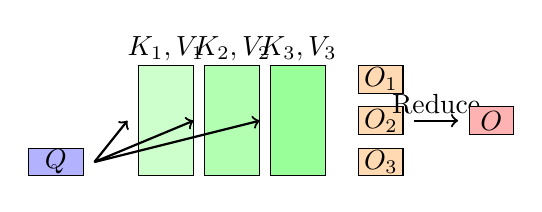
\begin{tikzpicture}[scale=0.7]
    % Q
    \draw[fill=blue!30] (0, 0) rectangle (1, 0.5);
    \node at (0.5, 0.25) {$Q$};

    % KV splits
    \draw[fill=green!20] (2, 0) rectangle (3, 2);
    \draw[fill=green!30] (3.2, 0) rectangle (4.2, 2);
    \draw[fill=green!40] (4.4, 0) rectangle (5.4, 2);
    \node at (2.5, 2.3) {$K_1, V_1$};
    \node at (3.7, 2.3) {$K_2, V_2$};
    \node at (4.9, 2.3) {$K_3, V_3$};

    % Parallel arrows
    \draw[->, thick] (1.2, 0.25) -- (1.8, 1);
    \draw[->, thick] (1.2, 0.25) -- (3, 1);
    \draw[->, thick] (1.2, 0.25) -- (4.2, 1);

    % Partial outputs
    \draw[fill=orange!30] (6, 1.5) rectangle (6.8, 2);
    \draw[fill=orange!30] (6, 0.75) rectangle (6.8, 1.25);
    \draw[fill=orange!30] (6, 0) rectangle (6.8, 0.5);
    \node at (6.4, 1.75) {$O_1$};
    \node at (6.4, 1) {$O_2$};
    \node at (6.4, 0.25) {$O_3$};

    % Reduce
    \draw[->, thick] (7, 1) -- (7.8, 1);
    \node at (7.4, 1.3) {Reduce};

    % Final output
    \draw[fill=red!30] (8, 0.75) rectangle (8.8, 1.25);
    \node at (8.4, 1) {$O$};
\end{tikzpicture}
\caption{Flash Decoding:KV序列并行 + Reduction}
\label{fig:flash_decoding}
\end{figure}

\subsubsection{性能提升}

\begin{itemize}
    \item 长序列解码加速高达\textbf{8倍}
    \item 在CodeLLaMa-34B上,注意力操作比FlashAttention快\textbf{50倍}
    \item 序列长度从512增加到64K,生成速度几乎不变
\end{itemize}

\subsection{FlashDecoding++}

FlashDecoding++~\citep{hong2024flashdecodingpp}进一步优化,在MLSys 2024发表。

\subsubsection{异步Softmax}

Flash Decoding的Reduction步骤需要同步等待所有部分结果。FlashDecoding++引入\textbf{Unified Max Value}:
\begin{itemize}
    \item 预估一个全局最大值$m_{unified}$(基于统计或启发式)
    \item 所有块使用相同的$m_{unified}$,无需同步
    \item 细粒度流水线,Prefill加速1.05$\times$,Decoding加速1.14$\times$
\end{itemize}

\subsubsection{Flat GEMM优化}

推理时的GEMM形状是``扁平''的($1 \times N$),标准实现效率低:
\begin{itemize}
    \item cuBLAS/CUTLASS对这种形状有高达50\%的性能损失
    \item FlashDecoding++使用Double Buffering和针对性优化
    \item Flat GEMM加速高达52\%
\end{itemize}

\subsubsection{启发式数据流}

根据输入形状动态选择最优数据流:
\begin{itemize}
    \item 不同序列长度、batch size有不同瓶颈
    \item 启发式选择避免静态数据流的50\%性能损失
\end{itemize}

\begin{table}[htbp]
\centering
\caption{Flash Decoding系列性能对比}
\label{tab:flash_decoding}
\begin{tabular}{lcc}
\toprule
方法 & 相对HuggingFace & 相对SOTA引擎 \\
\midrule
FlashAttention(推理) & 基线 & - \\
Flash Decoding & 8$\times$(长序列) & - \\
FlashDecoding++ & 4.86$\times$ & 1.37$\times$ \\
\bottomrule
\end{tabular}
\end{table}

\subsection{FlashAttention的工程影响}

FlashAttention已成为现代LLM训练和推理的\textbf{标配}:
\begin{itemize}
    \item \textbf{PyTorch 2.0+}:内置\texttt{scaled\_dot\_product\_attention}使用FlashAttention
    \item \textbf{vLLM、TensorRT-LLM}:推理引擎默认使用
    \item \textbf{所有主流LLM}:GPT-4、Claude、LLaMA、DeepSeek等都使用FlashAttention
\end{itemize}

\paragraph{上下文长度革命}
FlashAttention将实用上下文长度从2-4K提升到128K+:
\begin{itemize}
    \item 内存从$O(N^2)$降到$O(N)$
    \item 64K序列在标准注意力下需要16GB显存,FlashAttention只需约1GB
\end{itemize}

\begin{remark}[何时使用FlashAttention]
FlashAttention在以下场景收益最大:
\begin{itemize}
    \item \textbf{长序列}:序列长度$> 512$
    \item \textbf{大batch}:充分利用GPU并行
    \item \textbf{训练}:内存节省允许更大batch
\end{itemize}

短序列、小模型场景下,标准注意力可能更快(减少kernel launch开销)。
\end{remark}

\subsection{FlexAttention:可编程的FlashAttention}

FlexAttention是PyTorch 2.5引入的新API,提供FlashAttention的灵活编程接口。

\paragraph{动机}
FlashAttention虽然高效,但每种注意力变体(Causal、ALiBi、Sliding Window等)都需要专门实现。研究者想试验新变体时,往往需要手写Triton kernel。FlexAttention通过\texttt{torch.compile}自动生成高效kernel,将开发时间从数周缩短到数分钟。

\paragraph{核心API}
FlexAttention提供两个函数式接口:
\begin{itemize}
    \item \textbf{score\_mod}:修改$QK^\top$后的分数矩阵(如添加位置偏置)
    \item \textbf{mask\_mod}:定义mask模式(返回True的位置参与计算)
\end{itemize}

\begin{lstlisting}
from torch.nn.attention.flex_attention import flex_attention, create_block_mask

# Causal mask
def causal(b, h, q_idx, kv_idx):
    return q_idx >= kv_idx

# ALiBi位置编码
def alibi(score, b, h, q_idx, kv_idx):
    return score + (q_idx - kv_idx) * slope[h]

# 使用
block_mask = create_block_mask(causal, B, H, Q_LEN, KV_LEN)
out = flex_attention(q, k, v, score_mod=alibi, block_mask=block_mask)
\end{lstlisting}

\paragraph{性能}
FlexAttention达到FlashAttention-2约\textbf{85-90\%}的性能,但开发效率提升100倍。对于FlashAttention不原生支持的变体(如Document Masking),FlexAttention比标准SDPA快5-8倍。

\paragraph{适用场景}
\begin{itemize}
    \item 快速原型验证新的注意力变体
    \item 复杂mask模式(document masking、jagged tensors)
    \item 生产环境如果用标准变体,仍推荐直接使用FlashAttention
\end{itemize}


\newpage\section{Multi-head Latent Attention (MLA)}
\label{sec:mla}

FlashAttention解决了训练时注意力矩阵的IO瓶颈,但推理时还存在另一个内存挑战:\textbf{KV Cache}。自回归生成需要缓存所有历史token的Key和Value向量,随着上下文长度增加,这部分内存占用可能超过模型参数本身。

Multi-head Latent Attention(MLA)是DeepSeek-V2~\citep{deepseek2024v2}针对这一问题提出的解决方案。其核心洞察是:虽然每个注意力头需要独立的K和V,但它们可能存在\textbf{低秩结构}——即可以从一个共享的低维"潜在向量"中恢复。这种压缩不同于GQA/MQA的强制共享,而是让网络学习最优的压缩方式。

\subsection{背景与目标}

\subsubsection{KV Cache的挑战}

如第~\ref{sec:transformer_math}节所述,自回归生成时需要缓存历史的K和V:
\begin{equation}
    \text{KV Cache Size} = 2 \times B \times S \times L \times n_h \times d_h \times \text{bytes}
\end{equation}

对于大模型(如$n_h = 128$,$d_h = 128$),KV Cache成为长上下文推理的主要内存瓶颈。

\subsubsection{现有方案的局限}

\begin{table}[htbp]
\centering
\caption{KV Cache优化方案对比}
\label{tab:kv_cache_methods}
\begin{tabular}{lccc}
\toprule
Method & KV Cache Size & Performance & 原理 \\
\midrule
MHA & $2 n_h d_h$ & 最优 & 每头独立KV \\
GQA & $2 \frac{n_h}{g} d_h$ & 轻微下降 & $g$个Q头共享KV \\
MQA & $2 d_h$ & 明显下降 & 所有头共享KV \\
\textbf{MLA} & $d_c + d_h^R$ & \textbf{接近MHA} & 低秩压缩 \\
\bottomrule
\end{tabular}
\end{table}

GQA/MQA通过共享KV头来减少缓存,但这种强制共享往往损害模型性能。MLA的核心洞察是:\textbf{KV可以从一个低维潜在向量中恢复},而不必显式共享。

\subsection{MLA核心原理}

\subsubsection{低秩压缩思想}

MLA的核心思想是将高维的Key和Value压缩到一个共享的低维潜在向量(latent vector),推理时从该向量恢复K和V。

\begin{figure}[htbp]
\centering
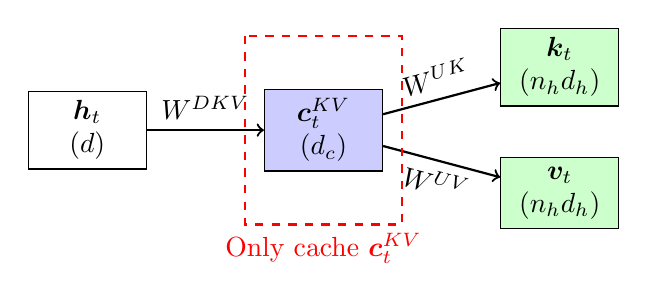
\begin{tikzpicture}[
    box/.style={rectangle, draw, minimum width=1.5cm, minimum height=0.8cm, align=center},
    arrow/.style={->, thick}
]
    % Input
    \node[box] (h) at (0,0) {$\bm{h}_t$\\$(d)$};

    % Compression
    \node[box, fill=blue!20] (c) at (3,0) {$\bm{c}_t^{KV}$\\$(d_c)$};

    % Decompression
    \node[box, fill=green!20] (k) at (6,0.8) {$\bm{k}_t$\\$(n_h d_h)$};
    \node[box, fill=green!20] (v) at (6,-0.8) {$\bm{v}_t$\\$(n_h d_h)$};

    % Arrows
    \draw[arrow] (h) -- node[above] {$W^{DKV}$} (c);
    \draw[arrow] (c) -- node[above, sloped] {$W^{UK}$} (k);
    \draw[arrow] (c) -- node[below, sloped] {$W^{UV}$} (v);

    % Cache indicator
    \draw[dashed, red, thick] (2,1.2) rectangle (4,-1.2);
    \node[red] at (3,-1.5) {Only cache $\bm{c}_t^{KV}$};
\end{tikzpicture}
\caption{MLA的KV压缩与恢复。只需缓存低维的$\bm{c}_t^{KV}$,K和V在计算时动态恢复。}
\label{fig:mla_compression}
\end{figure}

\subsection{数学公式}

\subsubsection{KV的低秩压缩}

对于输入 $\bm{h}_t \in \R^d$,首先压缩到潜在向量:
\begin{equation}
    \bm{c}_t^{KV} = W^{DKV} \bm{h}_t
    \label{eq:mla_compress}
\end{equation}
其中 $W^{DKV} \in \R^{d_c \times d}$ 是下投影矩阵,$d_c \ll n_h d_h$ 是压缩维度。

从潜在向量恢复K和V:
\begin{align}
    \bm{k}_t^C &= W^{UK} \bm{c}_t^{KV} \label{eq:mla_k} \\
    \bm{v}_t^C &= W^{UV} \bm{c}_t^{KV} \label{eq:mla_v}
\end{align}
其中 $W^{UK}, W^{UV} \in \R^{n_h d_h \times d_c}$ 是上投影矩阵。

\subsubsection{Query的低秩压缩}

类似地,Query也可以进行低秩压缩(主要用于减少训练时的激活内存):
\begin{align}
    \bm{c}_t^Q &= W^{DQ} \bm{h}_t \\
    \bm{q}_t^C &= W^{UQ} \bm{c}_t^Q
\end{align}
其中 $W^{DQ} \in \R^{d_c' \times d}$,$W^{UQ} \in \R^{n_h d_h \times d_c'}$。

\subsubsection{Decoupled RoPE}

RoPE需要在每个位置应用旋转,但如果直接对压缩后的$\bm{c}_t^{KV}$应用RoPE,会破坏后续的权重吸收优化。MLA采用\textbf{解耦RoPE}(Decoupled RoPE)策略:

\begin{enumerate}
    \item 将每个注意力头分为两部分:
    \begin{itemize}
        \item \textbf{内容部分}($d_h^C$维):从压缩向量恢复,\textbf{不}应用RoPE
        \item \textbf{位置部分}($d_h^R$维):额外投影,应用RoPE
    \end{itemize}

    \item 最终的Q和K为两部分的拼接:
    \begin{align}
        \bm{q}_t &= [\bm{q}_t^C; \text{RoPE}(\bm{q}_t^R, t)] \\
        \bm{k}_t &= [\bm{k}_t^C; \text{RoPE}(\bm{k}_t^R, t)]
    \end{align}
\end{enumerate}

其中位置部分的计算为:
\begin{align}
    \bm{q}_t^R &= W^{QR} \bm{c}_t^Q \\
    \bm{k}_t^R &= W^{KR} \bm{h}_t
\end{align}

\begin{remark}[为什么需要Decoupled RoPE]
RoPE是位置相关的:$\text{RoPE}(\bm{x}, t)$ 依赖于位置 $t$。如果对$\bm{c}_t^{KV}$应用RoPE再恢复K,则:
\[
    \bm{k}_t = W^{UK} \cdot \text{RoPE}(\bm{c}_t^{KV}, t)
\]
此时$W^{UK}$无法被吸收到$W^Q$中(因为RoPE在中间)。Decoupled策略将RoPE隔离到单独的维度,保留了权重吸收的可能性。
\end{remark}

\subsubsection{权重吸收}

MLA的一个关键优化是\textbf{权重吸收}(Weight Absorption)。由于压缩和恢复之间没有非线性激活,矩阵可以合并:

\paragraph{Query-Key吸收}
注意力分数的计算:
\begin{align}
    \bm{q}_t^{C\top} \bm{k}_s^C &= (\bm{c}_t^Q)^\top (W^{UQ})^\top W^{UK} \bm{c}_s^{KV} \\
    &= (\bm{c}_t^Q)^\top \underbrace{W^{QK}}_{\text{absorbed}} \bm{c}_s^{KV}
\end{align}
其中 $W^{QK} = (W^{UQ})^\top W^{UK} \in \R^{d_c' \times d_c}$。

\paragraph{Output-Value吸收}
输出投影的计算:
\begin{align}
    W^O \bm{v}_t^C &= W^O W^{UV} \bm{c}_t^{KV} \\
    &= \underbrace{W^{OV}}_{\text{absorbed}} \bm{c}_t^{KV}
\end{align}
其中 $W^{OV} = W^O W^{UV} \in \R^{d \times d_c}$。

\paragraph{推理流程}
权重吸收后,推理时:
\begin{enumerate}
    \item 缓存 $\bm{c}_t^{KV}$ 和 $\bm{k}_t^R$(位置部分)
    \item 用 $W^{QK}$ 直接计算内容部分的注意力分数
    \item 用吸收后的 $W^{OV}$ 计算输出
\end{enumerate}

\subsection{KV Cache分析}

\begin{table}[htbp]
\centering
\caption{MLA的KV Cache对比(per token per layer)}
\label{tab:mla_cache}
\begin{tabular}{lcc}
\toprule
Method & Cache Elements & DeepSeek-V2 (具体值) \\
\midrule
MHA & $2 n_h d_h$ & $2 \times 128 \times 128 = 32768$ \\
GQA (8组) & $2 \times 8 \times d_h$ & $2 \times 8 \times 128 = 2048$ \\
\textbf{MLA} & $d_c + d_h^R$ & $512 + 64 = 576$ \\
\bottomrule
\end{tabular}
\end{table}

DeepSeek-V2的配置:$d_c = 512$,$d_h^R = 64$,压缩比达到 $\frac{32768}{576} \approx \mathbf{56.9\times}$。

\subsection{PyTorch实现}

以下是MLA的简化PyTorch实现:

\begin{lstlisting}[language=Python, caption={MLA核心实现}]
import torch
import torch.nn as nn
import torch.nn.functional as F

class MultiHeadLatentAttention(nn.Module):
    def __init__(
        self,
        d_model: int,      # 模型维度
        n_heads: int,      # 注意力头数
        d_c: int,          # KV压缩维度
        d_c_q: int,        # Q压缩维度
        d_head_r: int,     # RoPE维度/头
    ):
        super().__init__()
        self.n_heads = n_heads
        self.d_head = d_model // n_heads
        self.d_c = d_c
        self.d_head_r = d_head_r

        # KV compression
        self.W_dkv = nn.Linear(d_model, d_c, bias=False)
        self.W_uk = nn.Linear(d_c, d_model, bias=False)
        self.W_uv = nn.Linear(d_c, d_model, bias=False)

        # Q compression
        self.W_dq = nn.Linear(d_model, d_c_q, bias=False)
        self.W_uq = nn.Linear(d_c_q, d_model, bias=False)

        # Decoupled RoPE projections
        self.W_qr = nn.Linear(d_c_q, n_heads * d_head_r, bias=False)
        self.W_kr = nn.Linear(d_model, n_heads * d_head_r, bias=False)

        # Output projection
        self.W_o = nn.Linear(d_model, d_model, bias=False)

    def forward(self, x, rope_fn, kv_cache=None):
        B, T, D = x.shape

        # KV compression: only c_kv needs caching
        c_kv = self.W_dkv(x)  # (B, T, d_c)

        # Decoupled RoPE keys
        k_r = self.W_kr(x)    # (B, T, n_heads * d_head_r)
        k_r = rope_fn(k_r)    # Apply RoPE

        # Handle KV cache
        if kv_cache is not None:
            c_kv_cached, k_r_cached = kv_cache
            c_kv = torch.cat([c_kv_cached, c_kv], dim=1)
            k_r = torch.cat([k_r_cached, k_r], dim=1)
        new_cache = (c_kv, k_r)

        # Q compression
        c_q = self.W_dq(x)    # (B, T, d_c_q)
        q_c = self.W_uq(c_q)  # (B, T, D) - content part
        q_r = self.W_qr(c_q)  # (B, T, n_heads * d_head_r) - RoPE part
        q_r = rope_fn(q_r)

        # Reconstruct K, V from compressed cache
        k_c = self.W_uk(c_kv)  # (B, S, D) - content part
        v = self.W_uv(c_kv)    # (B, S, D)

        # Reshape for multi-head attention
        q_c = q_c.view(B, T, self.n_heads, self.d_head)
        k_c = k_c.view(B, -1, self.n_heads, self.d_head)
        v = v.view(B, -1, self.n_heads, self.d_head)
        q_r = q_r.view(B, T, self.n_heads, self.d_head_r)
        k_r = k_r.view(B, -1, self.n_heads, self.d_head_r)

        # Concatenate content and RoPE parts
        q = torch.cat([q_c, q_r], dim=-1)  # (B, T, H, d_head + d_head_r)
        k = torch.cat([k_c, k_r], dim=-1)  # (B, S, H, d_head + d_head_r)

        # Scaled dot-product attention
        q, k, v = q.transpose(1,2), k.transpose(1,2), v.transpose(1,2)
        scale = (self.d_head + self.d_head_r) ** -0.5
        attn = F.softmax(q @ k.transpose(-2,-1) * scale, dim=-1)
        out = attn @ v  # (B, H, T, d_head)

        # Output projection
        out = out.transpose(1,2).reshape(B, T, D)
        out = self.W_o(out)

        return out, new_cache
\end{lstlisting}

\begin{remark}[实现优化]
上述代码为教学版本。实际部署时:
\begin{itemize}
    \item 权重吸收:预计算 $W^{QK} = (W^{UQ})^\top W^{UK}$ 和 $W^{OV} = W^O W^{UV}$
    \item Flash Attention:使用FlashAttention加速注意力计算
    \item 融合算子:将多个小矩阵乘法融合
\end{itemize}
\end{remark}

\subsection{MLA vs 其他方法}

\begin{table}[htbp]
\centering
\caption{注意力机制全面对比}
\label{tab:attention_comparison}
\begin{tabular}{lcccc}
\toprule
Feature & MHA & GQA & MQA & MLA \\
\midrule
KV Cache & $2n_h d_h$ & $2\frac{n_h}{g} d_h$ & $2 d_h$ & $d_c + d_h^R$ \\
参数量 & 基准 & 减少 & 最少 & 略增 \\
表达能力 & 最强 & 较强 & 较弱 & 接近MHA \\
推理延迟 & 高 & 中 & 低 & 中 \\
长上下文 & 受限 & 较好 & 好 & \textbf{最好} \\
\bottomrule
\end{tabular}
\end{table}

\paragraph{MLA的优势}
\begin{itemize}
    \item \textbf{极致压缩}:KV Cache减少93\%以上
    \item \textbf{性能保持}:不像GQA/MQA强制共享,而是学习最优压缩
    \item \textbf{长上下文友好}:128K上下文成为可能
\end{itemize}

\paragraph{MLA的代价}
\begin{itemize}
    \item \textbf{计算开销}:需要额外的压缩/恢复计算
    \item \textbf{实现复杂度}:Decoupled RoPE和权重吸收增加实现难度
    \item \textbf{训练成本}:低秩约束可能需要更多训练
\end{itemize}

\subsection{质量-效率权衡:何时使用MLA?}

MLA并非银弹。其56.9倍的压缩比来自于一个强假设:\textbf{K和V可以从512维潜在空间无损恢复}。这个假设在什么条件下成立?

\subsubsection{低秩假设的有效性}

考虑注意力模式的多样性需求。设任务需要 $r$ 种本质不同的注意力模式(如:局部依赖、长程依赖、语法结构、语义关联等),则KV表示至少需要 $r$ 个自由度。

\paragraph{压缩维度的下界}
若 $d_c < r$,则压缩会造成信息丢失。DeepSeek选择 $d_c = 512$,隐含假设是:常见NLP任务的注意力模式可以用不超过512维的空间表达。

\paragraph{任务依赖性}
不同任务对注意力多样性的需求不同:
\begin{itemize}
    \item \textbf{文本生成}:模式相对固定,低秩假设成立,MLA表现良好
    \item \textbf{代码理解}:需要追踪复杂的变量依赖和作用域,可能需要更高秩的表示
    \item \textbf{数学推理}:多步推理需要维持多条推理链,对注意力多样性要求高
\end{itemize}

\subsubsection{选择指南}

\begin{table}[htbp]
\centering
\caption{注意力机制选择指南}
\label{tab:attention_selection}
\begin{tabular}{lcc}
\toprule
场景 & 推荐方法 & 理由 \\
\midrule
长上下文推理 (>32K) & MLA & KV Cache是主要瓶颈 \\
短上下文、高吞吐 & GQA & 实现简单,开销低 \\
质量优先(小batch) & MHA & 无压缩损失 \\
代码/数学任务 & GQA或MHA & 注意力多样性需求高 \\
边缘设备部署 & MLA & 极致内存压缩 \\
\bottomrule
\end{tabular}
\end{table}

\paragraph{经验法则}
当 $\text{上下文长度} \times \text{batch size} > 10^6$ 时,KV Cache成为主要瓶颈,MLA的收益开始显现。对于短上下文或小batch推理,GQA的简单性可能更具优势。

\subsubsection{压缩比与质量的帕累托边界}

DeepSeek的消融实验表明,$d_c$ 的选择存在"甜点区":
\begin{itemize}
    \item $d_c < 256$:质量显著下降,压缩过度
    \item $d_c \in [256, 768]$:质量接近MHA,压缩有效
    \item $d_c > 768$:质量无进一步提升,压缩收益递减
\end{itemize}

$d_c = 512$ 处于帕累托最优附近——进一步压缩会损害质量,进一步扩大则浪费缓存空间。

\subsection{应用与扩展}

MLA已在以下模型中应用:
\begin{itemize}
    \item \textbf{DeepSeek-V2}:首次提出,236B参数MoE模型
    \item \textbf{DeepSeek-V3}:进一步优化,671B参数
    \item \textbf{DeepSeek-R1}:推理模型,继承MLA架构
\end{itemize}

\begin{remark}[MLA与MoE的协同]
MLA特别适合MoE架构:MoE的稀疏激活已经减少了计算量,而MLA进一步解决了内存瓶颈。两者结合使得DeepSeek-V2在保持高性能的同时,训练成本降低42.5\%。
\end{remark}

\newpage\section{稀疏注意力}
\label{sec:sparse-attention}

前两节介绍的FlashAttention和MLA分别从计算效率和内存占用角度优化了注意力机制,但它们都保留了完整的$O(N^2)$注意力计算——只是让这个计算更快、更省内存。本节探索另一条路径:如果大多数注意力权重本就接近零,我们能否\textbf{跳过这些无意义的计算}?

稀疏注意力的核心思想是:只计算"重要"的token对,将$O(N^2)$降至$O(Nk)$,其中$k \ll N$。与后面将介绍的线性注意力不同,稀疏注意力保留了精确的softmax计算,只是在更小的范围内进行。

\subsection{稀疏注意力概述}

\subsubsection{为什么需要稀疏注意力}

标准Softmax Attention的复杂度为$O(N^2)$,但实际上并非所有token对都同等重要:
\begin{itemize}
    \item 注意力分布通常是稀疏的(少数token获得大部分权重)
    \item 远距离token的注意力通常较弱
    \item 语义相关的token往往聚集在特定位置
\end{itemize}

稀疏注意力的核心思想:\textbf{只计算重要的注意力对},将复杂度从$O(N^2)$降至$O(Nk)$,其中$k \ll N$。

\subsubsection{稀疏注意力 vs 线性注意力}

\begin{table}[htbp]
\centering
\caption{稀疏注意力与线性注意力对比}
\label{tab:sparse_vs_linear}
\begin{tabular}{lcc}
\toprule
特性 & 稀疏注意力 & 线性注意力 \\
\midrule
复杂度 & $O(Nk)$ & $O(Nd^2)$ \\
注意力类型 & 精确Softmax & 近似/替代Softmax \\
长程精确检索 & 强 & 弱 \\
KV Cache & 需要完整 & 可压缩 \\
与原始Transformer兼容 & 高 & 中 \\
\bottomrule
\end{tabular}
\end{table}

\subsection{滑动窗口注意力}

滑动窗口注意力(Sliding Window Attention, SWA)是最直观的稀疏注意力形式:每个token只关注其周围固定窗口内的token。

\subsubsection{Mistral的滑动窗口~\citep{jiang2023mistral}}

Mistral 7B是首个将滑动窗口注意力规模化部署的开源模型,窗口大小为4096。

\paragraph{核心机制}
每个位置$t$的token只关注$[t-w, t]$范围内的token:
\begin{equation}
    \text{Attention}_t = \text{softmax}\left(\frac{q_t K_{[t-w:t]}^\top}{\sqrt{d}}\right) V_{[t-w:t]}
\end{equation}

\paragraph{层间信息传递}
滑动窗口的关键洞察是:通过Transformer的堆叠层,信息可以``跨窗口''传播。在第$k$层,位置$t$的token实际上可以访问到$[t - k \cdot w, t]$范围的信息。对于32层模型、窗口大小4096,理论感受野可达128K。

\paragraph{推理优化}
\begin{itemize}
    \item \textbf{滚动缓存}(Rolling Buffer):KV Cache只需保留最近$w$个token
    \item \textbf{内存节省}:8K序列长度下节省50\%缓存
    \item \textbf{速度提升}:配合FlashAttention和xFormers,16K序列上获得2倍加速
\end{itemize}

\subsubsection{Longformer与BigBird}

Longformer~\citep{beltagy2020longformer}和BigBird~\citep{zaheer2020bigbird}是早期将稀疏注意力系统化的工作。

\paragraph{Longformer}
结合三种注意力模式:
\begin{enumerate}
    \item \textbf{滑动窗口}:局部上下文建模
    \item \textbf{膨胀滑动窗口}(Dilated):扩大感受野
    \item \textbf{全局注意力}:特定token(如[CLS])关注全局
\end{enumerate}

\paragraph{BigBird}
在Longformer基础上增加\textbf{随机注意力}:
\begin{equation}
    A = A_{\text{sliding}} + A_{\text{global}} + A_{\text{random}}
\end{equation}
理论证明BigBird是完整注意力的通用近似器,支持最长8倍于BERT的序列。

\subsubsection{StreamingLLM~\citep{xiao2024streamingllm}}

StreamingLLM解决了一个重要问题:如何让LLM处理``无限长''的流式输入。

\paragraph{Attention Sink现象}
研究发现,无论输入多长,模型总是对\textbf{最开头的几个token}分配异常高的注意力权重——即使这些token在语义上并不重要。这被称为``注意力汇聚''(Attention Sink)。

\paragraph{SinkAttention}
StreamingLLM提出保留两部分KV Cache:
\begin{itemize}
    \item \textbf{Sink Tokens}:序列开头的4个token(固定)
    \item \textbf{滑动窗口}:最近的$w$个token
\end{itemize}
\begin{equation}
    \text{KV Cache} = \text{Sink}_{[1:4]} \cup \text{Window}_{[t-w:t]}
\end{equation}

\textbf{效果}:在4M+ token的流式场景下保持稳定性能,而普通滑动窗口在超过预训练长度后崩溃。

\subsection{KV Cache稀疏化}

KV Cache稀疏化是推理时的稀疏注意力:动态丢弃``不重要''的KV条目。

\subsubsection{H2O~\citep{zhang2024h2o}}

Heavy-Hitter Oracle(H2O)基于一个观察:少数``重击手''token累积了大部分注意力权重。

\paragraph{算法}
\begin{enumerate}
    \item 维护每个token的累积注意力分数
    \item 保留分数最高的Top-k token(Heavy Hitters)
    \item 结合最近的滑动窗口token
\end{enumerate}

\paragraph{层级策略}
不同层使用不同的保留策略,高层(更稀疏的注意力分布)可以更激进地压缩。

\subsubsection{SnapKV~\citep{li2024snapkv}}

SnapKV的核心洞察是:注意力模式在prefill阶段基本确定,可以``一次性''剪枝。

\paragraph{方法}
\begin{enumerate}
    \item 在prefill阶段末尾,分析最后一个窗口的注意力分布
    \item 识别整个上下文中的重要位置
    \item 永久保留这些位置的KV,丢弃其余
\end{enumerate}

\textbf{优势}:只需一次剪枝决策,无需每步动态更新。\\
\textbf{局限}:无法适应decoding阶段的动态变化。

\subsubsection{PyramidKV}

PyramidKV发现不同层的注意力稀疏度不同:
\begin{itemize}
    \item 低层:注意力较分散,需要更多KV
    \item 高层:注意力集中,可大幅压缩
\end{itemize}
因此采用\textbf{金字塔形}的KV分配:底层多、高层少。

\begin{table}[htbp]
\centering
\caption{KV Cache稀疏化方法对比}
\label{tab:kv_sparse}
\begin{tabular}{lccc}
\toprule
方法 & 剪枝时机 & 动态性 & 集成框架 \\
\midrule
H2O & 每步 & 动态 & vLLM \\
SnapKV & Prefill后 & 静态 & vLLM \\
StreamingLLM & 持续 & 静态 & -- \\
PyramidKV & 层级 & 静态 & -- \\
\bottomrule
\end{tabular}
\end{table}

\subsection{MoBA:块稀疏注意力}
\label{sec:moba}

MoBA(Mixture of Block Attention)~\citep{lu2025moba}是块级稀疏注意力的代表性工作,已部署于Kimi的长上下文服务。

\subsubsection{核心思想:将MoE应用于Attention}

MoBA的核心洞察是:\textbf{并非所有上下文对当前token都同等重要}。与其对整个序列计算注意力,不如让模型自主学习``关注哪些块''。

\paragraph{标准注意力}
\begin{equation}
    \text{Attn}(q, K, V) = \text{softmax}(qK^\top)V
\end{equation}

\paragraph{MoBA}
\begin{equation}
    \text{MoBA}(q, K, V) = \text{softmax}(qK_{[\mathcal{I}]}^\top)V_{[\mathcal{I}]}
    \label{eq:moba}
\end{equation}
其中$\mathcal{I} \subseteq [N]$是被选中的KV子集,由路由机制决定。

\subsubsection{块划分与路由机制}

\paragraph{块划分}
将长度为$N$的上下文均匀划分为$n$个块,每块大小$B = N/n$:
\begin{equation}
    \mathcal{I}_i = [(i-1) \cdot B + 1, \, i \cdot B], \quad i = 1, \ldots, n
\end{equation}

\paragraph{路由分数计算}
对每个query $q$,计算其与各块的亲和度分数:
\begin{equation}
    s_i = \langle q, \, \text{mean\_pool}(K_{[\mathcal{I}_i]}) \rangle
    \label{eq:moba_score}
\end{equation}
即query与块内所有key的平均向量的内积。这是一个\textbf{无参数}的路由机制。

\paragraph{Top-k选择}
选择分数最高的$k$个块进行注意力计算(典型设置$k = 3$):
\begin{equation}
    g_i = \begin{cases}
        1 & \text{if } s_i \in \text{Top-}k(\{s_j\}_{j=1}^n) \\
        0 & \text{otherwise}
    \end{cases}
\end{equation}

\subsubsection{因果性保证}

在自回归场景下:
\begin{enumerate}
    \item \textbf{未来块屏蔽}:对于位置$t$的query,所有$i > \lceil t/B \rceil$的块设$s_i = -\infty$
    \item \textbf{当前块强制选中}:query所在的块始终被路由
\end{enumerate}

\subsubsection{性能表现}

\begin{table}[htbp]
\centering
\caption{MoBA性能}
\label{tab:moba_performance}
\begin{tabular}{lcc}
\toprule
指标 & MoBA & Full Attention \\
\midrule
LM Loss差异 & \multicolumn{2}{c}{$< 10^{-3}$} \\
稀疏度 @32K & \multicolumn{2}{c}{95.31\%} \\
加速比 @1M & \multicolumn{2}{c}{6.5$\times$} \\
加速比 @10M & \multicolumn{2}{c}{16$\times$} \\
\bottomrule
\end{tabular}
\end{table}

\subsection{NSA:原生稀疏注意力}

Native Sparse Attention(NSA)~\citep{deepseek2025nsa}是DeepSeek提出的层级稀疏注意力机制,已部署于DeepSeek-V3.2。

\subsubsection{三条注意力路径}

NSA将注意力计算分解为三条并行路径:

\begin{figure}[htbp]
\centering
\begin{tikzpicture}[scale=0.7, font=\small]
    % Input
    \node[draw, rounded corners, fill=blue!20] (input) at (0, 0) {Query $q$};

    % Three paths
    \node[draw, rounded corners, fill=green!20] (comp) at (-4, -2) {Compression};
    \node[draw, rounded corners, fill=orange!20] (sel) at (0, -2) {Selection};
    \node[draw, rounded corners, fill=red!20] (sw) at (4, -2) {Sliding Window};

    % Arrows from input
    \draw[->, thick] (input) -- (comp);
    \draw[->, thick] (input) -- (sel);
    \draw[->, thick] (input) -- (sw);

    % Descriptions
    \node[below, text width=3cm, align=center] at (comp.south) {粗粒度\\块压缩};
    \node[below, text width=3cm, align=center] at (sel.south) {细粒度\\Top-k选择};
    \node[below, text width=3cm, align=center] at (sw.south) {局部\\滑动窗口};

    % Merge
    \node[draw, rounded corners, fill=purple!20] (merge) at (0, -5) {合并输出};
    \draw[->, thick] (comp) -- (merge);
    \draw[->, thick] (sel) -- (merge);
    \draw[->, thick] (sw) -- (merge);
\end{tikzpicture}
\caption{NSA的三条注意力路径}
\label{fig:nsa_paths}
\end{figure}

\paragraph{1. Compression Attention(压缩注意力)}
使用可学习的MLP将连续token压缩为块级表示:
\begin{equation}
    \tilde{K}_i = \text{MLP}(K_{[(i-1)l+1:il]}), \quad \tilde{V}_i = \text{MLP}(V_{[(i-1)l+1:il]})
\end{equation}
其中$l$是压缩块大小(NSA中$l=32$)。这捕获\textbf{全局粗粒度}信息。

\paragraph{2. Selection Attention(选择注意力)}
通过Lightning Indexer选择最相关的块保持原始精度:
\begin{enumerate}
    \item 计算query与所有块的相关性分数
    \item 选择Top-$n$个块(NSA中$n=16$个块,块大小$l'=64$)
    \item 对选中块进行精确Softmax注意力
\end{enumerate}
这保留\textbf{细粒度精确}信息。

\paragraph{3. Sliding Window Attention(滑动窗口注意力)}
对最近的$w$个token进行完整注意力(NSA中$w=512$):
\begin{equation}
    O_{sw} = \text{Attention}(q, K_{[t-w:t]}, V_{[t-w:t]})
\end{equation}
这保证\textbf{局部上下文}的精确建模。

\subsubsection{Lightning Indexer}

Lightning Indexer是NSA的核心创新,用于高效选择相关块:

\begin{itemize}
    \item 维护独立的\textbf{FP8量化}Key缓存(非MLA的KV Cache)
    \item 每个query计算与所有块的相关性分数
    \item 选择Top-k块(默认2048个token)
    \item 硬件优化:DeepGEMM实现的高效CUDA kernel
\end{itemize}

\textbf{关键设计}:索引计算与注意力计算分离,索引使用低精度快速完成。

\subsubsection{端到端可训练}

与ClusterKV、MagicPIG等依赖不可微操作的方法不同,NSA是\textbf{原生可训练}的——从预训练阶段就使用稀疏注意力。

\paragraph{可微的稀疏机制}
NSA的三个分支都支持梯度回传:
\begin{enumerate}
    \item \textbf{Token Compression}:可学习的MLP $\phi$将块级KV压缩为单个表示,带块内位置编码
    \item \textbf{Token Selection}:块重要性分数通过压缩token的注意力softmax计算,梯度可流过选择过程
    \item \textbf{门控机制}:通过MLP+Sigmoid学习三个分支的权重
\end{enumerate}

\paragraph{预训练配置}
DeepSeek使用27B参数模型(MoE架构,3B激活参数)验证NSA:
\begin{itemize}
    \item \textbf{模型规格}:30层,hidden\_dim=2560,GQA(4组,64头)
    \item \textbf{MoE结构}:72个路由专家 + 2个共享专家,top-k=6
    \item \textbf{训练数据}:270B tokens,8K序列长度
    \item \textbf{长上下文适配}:继续训练 + SFT在32K序列上,使用YaRN位置编码
\end{itemize}

\paragraph{训练加速}
NSA在训练阶段也实现了显著加速(64K序列长度,A100 GPU):
\begin{itemize}
    \item \textbf{前向传播}:9.0$\times$加速
    \item \textbf{反向传播}:6.0$\times$加速
    \item 加速比随序列长度增加:8K时4$\times$,16K时6.4$\times$,32K时9.1$\times$,64K时11.6$\times$
\end{itemize}

\paragraph{后训练:推理能力}
通过从DeepSeek-R1蒸馏,使用10B tokens的32K长度数学推理轨迹进行SFT。在AIME数学benchmark上,NSA-R比Full Attention-R提升+0.075,证明稀疏注意力不损害复杂推理能力。

\subsubsection{硬件对齐设计}

NSA针对现代GPU进行了深度优化,使用自定义Triton kernel:

\paragraph{Group-Centric Loading}
利用GQA的特性,将同一组内所有query head及其共享的稀疏KV块索引一次性加载到SRAM,避免重复内存访问。

\paragraph{Shared KV Fetching}
顺序加载被选中的连续KV块,最小化内存传输次数。由于不同query块的内循环长度几乎相同,可使用Triton的grid scheduler简化优化。

\paragraph{算术强度平衡}
通过组内共享消除冗余KV传输,在GPU流处理器间均衡计算负载,实现接近最优的算术强度。

\subsubsection{NSA参数配置}

\begin{table}[htbp]
\centering
\caption{NSA默认参数}
\label{tab:nsa_params}
\begin{tabular}{lcc}
\toprule
参数 & 符号 & 值 \\
\midrule
压缩块大小 & $l$ & 32 \\
选择块大小 & $l'$ & 64 \\
选择块数量 & $n$ & 16 \\
滑动窗口大小 & $w$ & 512 \\
滑动步长 & $d$ & 16 \\
\bottomrule
\end{tabular}
\end{table}

\subsection{DSA:DeepSeek稀疏注意力}

DSA(DeepSeek Sparse Attention,2025年9月)是DeepSeek在V3.2中部署的新一代稀疏注意力,与NSA有本质区别。DSA摒弃了NSA复杂的三分支设计,采用更简洁的\textbf{细粒度token级检索}。

\subsubsection{与NSA的核心区别}

\begin{table}[htbp]
\centering
\caption{NSA vs DSA设计对比}
\label{tab:nsa_vs_dsa}
\begin{tabular}{lcc}
\toprule
特性 & NSA & DSA \\
\midrule
选择粒度 & 块级(block) & Token级 \\
分支数量 & 3(压缩+选择+窗口) & 1(直接选择) \\
重要度计算 & 可学习MLP & 可学习$w$权重 \\
Attention变种 & GQA & MLA \\
验证模型 & 27B & 671B \\
\bottomrule
\end{tabular}
\end{table}

\subsubsection{算法设计}

DSA的核心思想:每个query只需关注固定数量$k$个最相关的token($k=2048$)。

\paragraph{重要度分数计算}
DSA引入可学习权重$w$计算token重要度:
\begin{equation}
    \text{score}_i = w \cdot f(q, k_i)
\end{equation}
这是一个折中方案——比NSA的MLP简单,但比MoBA的无参数mean-pooling更有表达力。

\paragraph{Top-k检索}
根据重要度分数选择Top-$k$个token进行精确注意力计算:
\begin{equation}
    \mathcal{I} = \text{Top-}k(\{\text{score}_i\}_{i=1}^N), \quad |\mathcal{I}| = 2048
\end{equation}

\paragraph{复杂度分析}
单query需访问固定$k$个token,因此整体复杂度为$O(Nk)$,是真正的\textbf{线性复杂度}。

\subsubsection{训练挑战与解决}

细粒度token级检索比块级更难训练。DSA采用以下技巧:
\begin{itemize}
    \item \textbf{Warm-up}:逐步增加稀疏度
    \item \textbf{知识蒸馏}:从Full Attention模型蒸馏
    \item \textbf{MLA适配}:专门针对Multi-Latent Attention优化
\end{itemize}

\subsubsection{工程实现}

\begin{itemize}
    \item \textbf{TileLang Kernel}:细粒度稀疏+MLA需要定制kernel,TileLang比Triton性能更优
    \item \textbf{vLLM/SGLang集成}:Day-0支持,使用DeepGEMM和FlashMLA
    \item \textbf{Blackwell优化}:与NVIDIA合作优化B200
\end{itemize}

\subsubsection{性能收益}

\begin{itemize}
    \item 长上下文API成本降低约\textbf{50\%}
    \item 64K序列上实现显著加速
    \item 671B模型上验证,质量几乎无损
\end{itemize}

\subsection{NSA vs MoBA vs DSA:三种方法深度对比}

2025年出现了三种重要的``学习式''稀疏注意力方法。本节从多个维度进行详细对比。

\subsubsection{算法设计对比}

\begin{table}[htbp]
\centering
\caption{三种方法算法设计对比}
\label{tab:three_algo_comparison}
\begin{tabular}{lccc}
\toprule
设计维度 & NSA & MoBA & DSA \\
\midrule
\multicolumn{4}{l}{\textit{基本信息}} \\
发布时间 & 2025.02 & 2025.02 & 2025.09 \\
提出者 & DeepSeek & Moonshot (Kimi) & DeepSeek \\
Attention基础 & GQA & GQA & MLA \\
\midrule
\multicolumn{4}{l}{\textit{稀疏策略}} \\
选择粒度 & 块级 & 块级 & Token级 \\
分支数量 & 3(压缩+选择+窗口) & 1 & 1 \\
路由机制 & 可学习MLP & 无参数mean-pool & 可学习$w$ \\
局部窗口 & 有($w$=512) & 当前块强制选中 & 无 \\
\bottomrule
\end{tabular}
\end{table}

\subsubsection{超参数与复杂度对比}

\begin{table}[htbp]
\centering
\caption{超参数与复杂度对比}
\label{tab:three_params_comparison}
\begin{tabular}{lccc}
\toprule
参数 & NSA & MoBA & DSA \\
\midrule
\multicolumn{4}{l}{\textit{关键超参}} \\
块大小 & $l$=32, $l'$=64 & $L$=4096 & -- \\
选择数量 & $n$=16块 & $k$=12块 & $k$=2048 tokens \\
滑动窗口 & $w$=512 & -- & -- \\
\midrule
\multicolumn{4}{l}{\textit{单query访问token数}} \\
@32K上下文 & $\sim$2560 & 49152 & 2048 \\
@128K上下文 & $\sim$5120 & 49152 & 2048 \\
是否随$N$增长 & 是($O(N/L)$) & 否(固定$kL$) & 否(固定$k$) \\
\midrule
\multicolumn{4}{l}{\textit{复杂度(vs原版$O(N^2)$)}} \\
理论复杂度 & $O(N^2/L)$ & $O(N \cdot kL)$ & $O(Nk)$ \\
实际系数 & $O(N^2/32)$ & $O(N \cdot 49152)$ & $O(N \cdot 2048)$ \\
@64K稀疏度 & $\sim$97\% & $\sim$23\% & $\sim$97\% \\
\bottomrule
\end{tabular}
\end{table}

\subsubsection{重要度计算机制}

三种方法采用不同的``检索''策略来确定哪些token值得关注:

\paragraph{NSA:可学习MLP压缩}
\begin{equation}
    \tilde{k}_i = \text{MLP}(K_{[(i-1)l+1:il]}), \quad \text{score}_i = q \cdot \tilde{k}_i
\end{equation}
使用一个额外的MLP将块内所有key压缩为单个表示,再计算与query的相似度。\textbf{优点}:表达力强。\textbf{缺点}:引入额外参数和计算。

\paragraph{MoBA:无参数Mean-Pooling}
\begin{equation}
    \text{score}_i = q \cdot \text{mean}(K_{[(i-1)L+1:iL]})
\end{equation}
直接对块内key做平均,再与query内积。\textbf{优点}:无额外参数,简洁优雅。\textbf{缺点}:表达力受限,块内信息被``抹平''。

\paragraph{DSA:可学习权重$w$}
\begin{equation}
    \text{score}_i = w \cdot f(q, k_i)
\end{equation}
介于两者之间——有可学习参数,但比MLP简单。\textbf{优点}:平衡表达力与复杂度。\textbf{缺点}:具体形式未完全公开。

\subsubsection{训练与工程对比}

\begin{table}[htbp]
\centering
\caption{训练与工程实现对比}
\label{tab:three_training_comparison}
\begin{tabular}{lccc}
\toprule
维度 & NSA & MoBA & DSA \\
\midrule
\multicolumn{4}{l}{\textit{训练}} \\
训练方式 & 原生预训练 & 继续训练 & 原生预训练 \\
验证模型规模 & 27B & 8B & 671B \\
训练数据量 & 270B tokens & -- & -- \\
训练序列长度 & 8K$\to$32K & -- & -- \\
需要蒸馏 & 可选(R1蒸馏) & 否 & 是(关键) \\
需要Warm-up & 否 & 否 & 是(关键) \\
\midrule
\multicolumn{4}{l}{\textit{工程实现}} \\
Kernel实现 & Triton & Triton & TileLang \\
与MLA兼容 & 否 & 否 & 是 \\
推理框架支持 & -- & -- & vLLM/SGLang \\
\midrule
\multicolumn{4}{l}{\textit{加速效果}} \\
前向加速@64K & 9$\times$ & 6.5$\times$@1M & -- \\
后向加速@64K & 6$\times$ & -- & -- \\
解码加速@64K & 11.6$\times$ & 16$\times$@10M & -- \\
\bottomrule
\end{tabular}
\end{table}

\subsubsection{设计哲学差异}

\paragraph{NSA:全面覆盖,层级融合}
NSA的设计理念是\textbf{不遗漏任何重要信息}:
\begin{itemize}
    \item \textbf{压缩分支}:捕获全局粗粒度信息
    \item \textbf{选择分支}:保留细粒度精确信息
    \item \textbf{窗口分支}:确保局部上下文不丢失
    \item 三分支通过可学习门控融合
\end{itemize}
\textbf{代价}:超参较多($l$, $l'$, $n$, $w$, $d$, 门控参数),调优和迁移复杂。

\paragraph{MoBA:简洁优雅,MoE思想}
MoBA的设计理念是\textbf{将MoE的路由思想应用于Attention}:
\begin{itemize}
    \item 把KV Cache视为``专家池'',每个块是一个``专家''
    \item 无参数路由,让注意力分数自然决定选择
    \item 当前块强制选中,保证局部信息
\end{itemize}
\textbf{优势}:设计最简洁,与现有架构兼容性好。很多人认为MoBA更有潜力成为下一代Transformer的基础组件。\\
\textbf{疑问}:块大小4096较大(约1页PDF),是否会退化为sliding window等trivial模式?

\paragraph{DSA:激进稀疏,端到端优化}
DSA的设计理念是\textbf{极限稀疏+精心训练}:
\begin{itemize}
    \item Token级选择,每个query只看2048个token(约3\%@64K)
    \item 与MLA深度集成,需要定制TileLang kernel
    \item 训练难度大,依赖warm-up和蒸馏
\end{itemize}
\textbf{优势}:稀疏度最高,推理效率最好,在671B超大模型上验证。\\
\textbf{挑战}:Token级检索是否会遗漏关键信息?小模型能否复现?

\subsubsection{稀疏模式可视化理解}

假设上下文长度$N$=32K,三种方法的稀疏模式差异:

\begin{table}[htbp]
\centering
\caption{@32K上下文的稀疏模式}
\label{tab:sparsity_pattern}
\begin{tabular}{lccc}
\toprule
特性 & NSA & MoBA & DSA \\
\midrule
块数量 & 1024块(每块32 token) & 8块(每块4096 token) & 32K个token \\
选中数量 & 16块+窗口 & 12块 & 2048 token \\
选中token数 & $\sim$2560 & $\sim$49152 & 2048 \\
稀疏度 & 92\% & 0\%(看全部) & 94\% \\
\bottomrule
\end{tabular}
\end{table}

\textbf{关键观察}:在32K这个长度上,MoBA实际上几乎没有稀疏(选中12块$\times$4096=49152 > 32K)!MoBA的稀疏优势在更长序列(如128K+)才能体现。

\subsubsection{适用场景建议}

\begin{table}[htbp]
\centering
\caption{适用场景建议}
\label{tab:when_to_use}
\begin{tabular}{lp{10cm}}
\toprule
方法 & 适用场景 \\
\midrule
NSA & 需要精确保留多尺度信息;可接受复杂超参调优;使用GQA架构 \\
MoBA & 追求简洁设计;希望无缝替换现有Attention;序列长度128K+ \\
DSA & 使用MLA架构;追求极致稀疏度;有足够资源做蒸馏训练;超大模型(100B+) \\
\bottomrule
\end{tabular}
\end{table}

\subsubsection{开放问题与未来方向}

\paragraph{固定$k$是否合理?}
DSA和MoBA都假设每个query只需看固定数量的token,不随$N$增长。这个假设值得深思:
\begin{itemize}
    \item \textbf{反对观点}:上下文很长时,固定$k$可能遗漏关键信息。Needle-in-haystack任务可能受影响。
    \item \textbf{支持观点}:每个token的``信息容量''有限。人类阅读长文档时也不会逐字关注。
    \item \textbf{折中思路}:可能需要自适应$k$,或结合全局压缩分支(如NSA)。
\end{itemize}

\paragraph{稀疏度应该自适应吗?}
目前三种方法的稀疏度都是人为设定的超参。未来方向可能包括:
\begin{itemize}
    \item 不同层使用不同稀疏度(类似PyramidKV的思想)
    \item 不同query根据任务复杂度动态调整$k$
    \item 通过强化学习或可微搜索自动确定稀疏策略
\end{itemize}

\paragraph{稀疏 vs 压缩:两条技术路线}
\begin{itemize}
    \item \textbf{稀疏路线}(NSA/MoBA/DSA):动态``检索''重要token,不改变KV Cache大小
    \item \textbf{压缩路线}(Qwen3-Next线性注意力):压缩KV Cache本身,信息更紧凑
    \item 两者可能结合:先压缩再稀疏,或用稀疏注意力指导压缩
\end{itemize}

\paragraph{Post-training方法是否被``降维打击''?}
原生稀疏注意力(NSA/DSA)的出现,对H2O、SnapKV、Quest等post-training稀疏方法形成挑战:
\begin{itemize}
    \item Post-training方法:在已训练好的模型上``事后''稀疏化
    \item 原生方法:从预训练开始就使用稀疏注意力
    \item 原生方法的优势:模型从一开始就学会``如何稀疏'',效果更好
    \item Post-training方法的优势:可应用于任意已有模型,无需重新训练
\end{itemize}

\subsection{Ring Attention与上下文并行}

当序列长度超过单GPU显存容量时,需要将注意力计算分布到多个设备上。

\subsubsection{Ring Attention~\citep{liu2023ringattention}}

Ring Attention将长序列分割到多个GPU,通过环形通信实现分布式注意力计算。

\paragraph{算法流程}
\begin{enumerate}
    \item 将Query、Key、Value按序列维度分割到$P$个GPU
    \item 每个GPU持有本地Query块,计算与本地KV的注意力
    \item KV块在GPU之间环形传递,累积计算全局注意力
    \item 使用online softmax避免数值溢出
\end{enumerate}

\paragraph{通信隐藏}
关键优化是\textbf{计算-通信重叠}:在计算当前KV块注意力的同时,异步传递下一个KV块。

\subsubsection{LLaMA 3的上下文并行}

LLaMA 3训练采用All-Gather方式的Context Parallelism~\citep{dubey2024llama3}:
\begin{itemize}
    \item 先All-Gather收集所有KV,再计算本地Query的注意力
    \item 为负载均衡,将序列分为$2 \times \text{CP}$个块并shuffle
    \item 支持128K上下文的高效训练
\end{itemize}

\paragraph{与Ring Attention对比}
\begin{itemize}
    \item Ring Attention:点对点通信,延迟可隐藏
    \item All-Gather:集合通信,实现更简单但延迟在关键路径
\end{itemize}

\subsection{稀疏注意力方法全景}

\begin{table}[htbp]
\centering
\caption{稀疏注意力方法全景对比}
\label{tab:sparse_comparison}
\begin{tabular}{lccccc}
\toprule
方法 & 稀疏策略 & 复杂度 & 全局信息 & 部署 \\
\midrule
Sliding Window & 固定窗口 & $O(Nw)$ & 无 & Mistral \\
Longformer & 窗口+全局 & $O(N(w+g))$ & 全局token & Longformer \\
BigBird & 窗口+全局+随机 & $O(N(w+g+r))$ & 全局+随机 & BigBird \\
StreamingLLM & Sink+窗口 & $O(N(s+w))$ & Sink tokens & -- \\
MoBA & 块路由 & $O(N \cdot kL)$ & Top-k块 & Kimi \\
NSA & 压缩+选择+窗口 & $O(N^2/L)$ & 压缩+选择 & -- \\
DSA & Token级检索 & $O(Nk)$ & Top-k token & DeepSeek-V3.2 \\
Ring Attention & 分布式 & $O(N^2/P)$ & 完整 & LLaMA 3 \\
\bottomrule
\end{tabular}
\end{table}

\begin{remark}[稀疏注意力的演进]
从Longformer/BigBird的``手工设计模式''到MoBA/NSA/DSA的``学习式稀疏'',稀疏注意力正经历范式转变。2025年,稀疏注意力首次在600B+规模模型上得到验证(DeepSeek-V3.2),标志着该技术从学术研究走向工业主流。
\end{remark}

\subsection{与其他方法的关系}

\subsubsection{与FlashAttention的关系}

稀疏注意力与FlashAttention是\textbf{正交}的优化:
\begin{itemize}
    \item FlashAttention优化\textbf{IO效率}(不改变计算量)
    \item 稀疏注意力减少\textbf{计算量}(只计算部分注意力)
    \item 两者可以结合:对选中的稀疏token使用FlashAttention计算
\end{itemize}

\subsubsection{与KV Cache压缩的关系}

\begin{itemize}
    \item \textbf{KV Cache压缩}(如SnapKV、H2O):推理时丢弃不重要的KV
    \item \textbf{稀疏注意力}:训练和推理时都只计算部分注意力
    \item 稀疏注意力是更根本的解决方案,从架构层面减少计算
\end{itemize}

\subsection{实践建议}

\paragraph{何时使用稀疏注意力}
\begin{itemize}
    \item 长上下文场景(32K+)
    \item 需要精确检索能力(passkey retrieval等)
    \item 希望保持Softmax注意力的特性
\end{itemize}

\paragraph{何时使用线性注意力}
\begin{itemize}
    \item 超长上下文(1M+)
    \item KV Cache显存受限
    \item 可以接受一定的精度损失
\end{itemize}

\begin{remark}[稀疏注意力的发展趋势]
稀疏注意力正从``手工设计模式''(如固定滑动窗口)向``学习式稀疏''演进:
\begin{itemize}
    \item MoBA:无参数路由,让模型学习关注哪些块
    \item NSA:可学习的压缩和选择机制
    \item 未来:更细粒度、更自适应的稀疏策略
\end{itemize}
\end{remark}


\newpage\section{线性注意力}
\label{sec:linear-attention}

稀疏注意力通过"只计算重要的token对"将$O(N^2)$降至$O(Nk)$,但它仍然保留了softmax的计算形式。本节介绍一条更激进的路径:\textbf{彻底改变注意力的数学形式},使复杂度降至真正的$O(N)$。

线性注意力的核心洞察是:softmax注意力之所以需要$O(N^2)$,是因为必须先算出完整的$N \times N$注意力矩阵再做归一化。如果我们用其他函数替代softmax,使得计算可以"重新排列",就能避免显式构造这个矩阵。这种重排不是免费的——我们用数学等价性换取计算效率,代价是改变了注意力的语义。

\subsection{核心思想}

\subsubsection{从Softmax Attention到线性化}

标准自注意力(单头)的计算为:
\begin{equation}
    \text{Attention}(Q, K, V) = \underbrace{\text{softmax}\left(\frac{QK^\top}{\sqrt{d}}\right)}_{n \times n} V
\end{equation}
其中需要显式构造$n \times n$的注意力矩阵,时间和空间复杂度均为$O(n^2)$。

线性注意力的核心思想是:将softmax或$QK^\top$改写为可分解的形式,利用乘法结合律改变计算顺序:
\begin{equation}
    \text{Attention}(Q, K, V) \approx \phi(Q) \cdot \underbrace{(\phi(K)^\top V)}_{d \times d}
    \label{eq:linear_attn_kernel}
\end{equation}
其中$\phi(\cdot)$是某种特征映射函数。关键在于:先计算$\phi(K)^\top V$(与长度$n$线性相关的$d \times d$矩阵),再左乘$\phi(Q)$,总复杂度降为$O(nd^2)$,当$d \ll n$时近似$O(n)$。

\subsubsection{递推形式:Transformer即RNN}

在自回归(causal)场景下,线性注意力可以写成类似RNN的递推式~\citep{katharopoulos2020linear}。设$q_t, k_t, v_t$分别为第$t$步的query、key、value向量,定义状态矩阵$S_t \in \R^{d \times d}$:
\begin{align}
    S_t &= S_{t-1} + v_t k_t^\top \\
    o_t &= S_t \cdot q_t
    \label{eq:linear_attn_rnn}
\end{align}
这揭示了一个深刻联系:\textbf{线性Attention本质上是一种RNN},其隐状态$S_t$累积了历史信息。

\begin{remark}[线性注意力的双模式]
线性注意力支持两种等价的计算模式:
\begin{itemize}
    \item \textbf{并行模式}:训练时使用矩阵乘法,充分利用GPU并行性
    \item \textbf{递推模式}:推理时使用RNN形式,实现$O(1)$的增量更新
\end{itemize}
这种双模式特性使线性注意力在训练和推理阶段都能获得最优效率。
\end{remark}

\subsection{经典线性注意力方法}

\subsubsection{Linear Transformer~\citep{katharopoulos2020linear}}

最早系统化提出``Transformer即RNN''的工作。核心思想是将softmax attention重写为核函数形式:
\begin{equation}
    \text{Attention}(Q, K, V) = \frac{\phi(Q) (\phi(K)^\top V)}{\phi(Q) (\phi(K)^\top \bm{1})}
\end{equation}
其中$\phi(x) = \text{elu}(x) + 1$保证非负性。实验表明在自回归任务上可获得高达4000倍的加速。

\textbf{局限}:简单的特征映射难以精确近似softmax的行为,在复杂语言任务上存在性能差距。

\subsubsection{Performer~\citep{choromanski2020performer}}

提出FAVOR+(Fast Attention Via positive Orthogonal Random features)方法,用随机特征近似softmax核:
\begin{equation}
    \text{softmax}(q^\top k) \approx \phi(q)^\top \phi(k)
\end{equation}
其中$\phi$通过正交随机特征构造,具有无偏或近似无偏的理论保证。

\textbf{优势}:与原始Transformer完全兼容,可作为drop-in replacement。\\
\textbf{局限}:随机近似在实际任务中仍有精度损失。

\subsubsection{cosFormer~\citep{qin2022cosformer}}

不再硬近似softmax,而是基于softmax的两个关键性质设计线性替代:
\begin{enumerate}
    \item \textbf{非负性}:注意力权重应为非负
    \item \textbf{分布集中性}:注意力应集中在相关位置
\end{enumerate}

cosFormer使用ReLU保证非负性,并引入基于余弦的位置再加权机制:
\begin{equation}
    \text{Attention}_{ij} = \text{ReLU}(q_i)^\top \text{ReLU}(k_j) \cdot \cos\left(\frac{\pi}{2} \cdot \frac{i - j}{n}\right)
\end{equation}

在Long-Range Arena等长序列benchmark上取得当时最优性能,是``好用的线性Attention''的代表。

\subsection{带遗忘门的线性注意力}

原始线性注意力的一个根本问题是:状态矩阵$S_t$只能累加,无法遗忘。随着序列增长,历史信息``挤在一起'',导致检索能力下降。

\subsubsection{RetNet~\citep{sun2023retnet}}

微软提出的Retentive Network引入指数衰减因子$\gamma \in (0, 1)$:
\begin{align}
    S_t &= \gamma S_{t-1} + v_t k_t^\top \\
    o_t &= S_t \cdot q_t
    \label{eq:retnet}
\end{align}
这相当于对历史信息施加指数衰减,强调近期token的重要性。

\textbf{Multi-Scale Retention}:不同attention head使用不同的$\gamma$值,实现多尺度的记忆保持:
\begin{itemize}
    \item 小$\gamma$:关注近期信息(短程依赖)
    \item 大$\gamma$:保留更长历史(长程依赖)
\end{itemize}

\textbf{三种计算模式}:
\begin{enumerate}
    \item \textbf{并行模式}:训练时的矩阵计算
    \item \textbf{递推模式}:$O(1)$推理
    \item \textbf{分块递推模式}:长序列的高效处理
\end{enumerate}

性能:7B模型在8k序列长度下,推理速度比Transformer快8.4倍,内存减少70\%。

\subsubsection{Lightning Attention~\citep{minimax2025}}

MiniMax提出的Lightning Attention是目前\textbf{首个规模化到商业级的线性注意力架构}。核心创新:

\textbf{分块计算策略}:将注意力计算分为intra-block和inter-block两部分:
\begin{itemize}
    \item \textbf{Intra-block}:块内使用``左乘''形式,可并行计算
    \item \textbf{Inter-block}:块间使用``右乘''形式,累积状态
\end{itemize}
这种分解避免了传统线性注意力中缓慢的cumsum操作。

\textbf{混合架构}:每8层中,7层使用Lightning Attention,1层使用标准Softmax Attention,平衡效率与精度。

\begin{table}[htbp]
\centering
\caption{MiniMax-01模型规格}
\label{tab:minimax_spec}
\begin{tabular}{lc}
\toprule
参数 & 值 \\
\midrule
总参数量 & 456B \\
激活参数量(MoE) & 45.9B \\
专家数量 & 32 \\
训练上下文长度 & 1M tokens \\
推理外推长度 & 4M tokens \\
\bottomrule
\end{tabular}
\end{table}

\subsection{DeltaNet:基于Delta Rule的线性注意力}

\subsubsection{动机:解决记忆过载问题}

原始线性注意力的核心缺陷是\textbf{记忆过载}(memory overload):只能添加新的key-value关联,无法擦除已有信息。这导致随着序列增长,检索错误累积。

\subsubsection{Delta Rule更新}

DeltaNet~\citep{yang2024deltanet}引入``除旧迎新''的Delta Rule:
\begin{equation}
    S_t = S_{t-1} - \underbrace{(S_{t-1} \cdot k_t - v_t)}_{\text{delta}} \cdot k_t^\top
    \label{eq:deltanet}
\end{equation}

直观理解:
\begin{enumerate}
    \item $S_{t-1} \cdot k_t$:用当前key检索记忆中的value
    \item $S_{t-1} \cdot k_t - v_t$:计算检索值与真实值的差异(delta)
    \item 根据delta修正记忆,实现``精准更新''
\end{enumerate}

\subsubsection{Gated DeltaNet~\citep{yang2025gateddeltan}}

ICLR 2025工作进一步引入门控机制:
\begin{equation}
    S_t = \alpha_t \odot S_{t-1} + \beta_t \odot (v_t - S_{t-1} \cdot k_t) \cdot k_t^\top
\end{equation}
其中$\alpha_t$控制遗忘,$\beta_t$控制更新强度。

\textbf{互补性}:门控实现快速记忆擦除,Delta Rule实现精准记忆更新,两者结合在多个benchmark上超越Mamba2和原始DeltaNet。

\textbf{工业采用}:Gated DeltaNet已被Qwen3-Next采用作为线性注意力层。

\subsection{与状态空间模型的联系}

\subsubsection{Mamba与结构化状态空间对偶}

Mamba~\citep{gu2023mamba}是另一条重要的高效序列建模路线,基于选择性状态空间模型(Selective SSM)。Mamba-2论文~\citep{dao2024mamba2}揭示了\textbf{结构化状态空间对偶}(Structured State Space Duality, SSD):

\begin{quote}
    ``与标准自注意力相比,SSD只有两个区别:去掉softmax归一化,并应用一个独立的逐元素掩码矩阵。''
\end{quote}

这表明线性注意力和SSM可以视为同一框架的不同实例:
\begin{itemize}
    \item 线性注意力:通过特征映射分解attention矩阵
    \item SSM:通过状态空间方程建模序列
    \item 两者都有线性复杂度和递推形式
\end{itemize}

\subsubsection{混合架构}

实践中,纯线性模型在某些任务上仍有差距,因此出现了混合架构:
\begin{itemize}
    \item \textbf{Jamba}(AI21):Mamba + Attention
    \item \textbf{MiniMax-01}:Lightning Attention + 稀疏Softmax Attention
    \item \textbf{Qwen3-Next}:Gated DeltaNet + SwiGLU
\end{itemize}

\subsection{Test-Time Training视角}

苏剑林在``线性注意力简史''~\citep{su2025linearhistory}中指出,现代线性注意力的核心思想可以统一到\textbf{Test-Time Training}(TTT)框架:

\begin{quote}
    ``将序列建模视为在线学习问题,用优化器构建RNN。不同的损失函数对应不同的RNN模型。''
\end{quote}

\begin{table}[htbp]
\centering
\caption{线性注意力方法的TTT视角}
\label{tab:ttt_view}
\begin{tabular}{lll}
\toprule
方法 & 更新规则 & 对应优化器 \\
\midrule
Linear Attention & $S_t = S_{t-1} + v_t k_t^\top$ & 累积梯度 \\
RetNet & $S_t = \gamma S_{t-1} + v_t k_t^\top$ & 带衰减的累积 \\
DeltaNet & $S_t = S_{t-1} - (S_{t-1}k_t - v_t)k_t^\top$ & Delta Rule \\
Gated DeltaNet & 门控Delta Rule & 自适应学习率 \\
\bottomrule
\end{tabular}
\end{table}

这个视角为设计新型线性注意力提供了原则性指导:选择合适的``优化器''来更新记忆状态。

\subsection{工业部署现状}

\begin{table}[htbp]
\centering
\caption{线性注意力的工业应用}
\label{tab:linear_attn_industry}
\begin{tabular}{llll}
\toprule
公司/模型 & 架构类型 & 上下文长度 & 特点 \\
\midrule
MiniMax-01 & Lightning Attention + MoE & 1M-4M & 首个商业级线性Attention LLM \\
MiniMax-M1 & Lightning Attention & 1M+80k生成 & 开源reasoning模型 \\
Qwen3-Next & Gated DeltaNet & -- & 线性层 + 门控Attention \\
\bottomrule
\end{tabular}
\end{table}

\textbf{关键观察}:MiniMax是目前唯一将线性注意力规模化到商业级的厂商。其他厂商(如Kimi、DeepSeek)更倾向于稀疏注意力路线(见第\ref{sec:sparse-attention}节)。

\subsection{线性注意力的局限与展望}

\paragraph{当前局限}
\begin{enumerate}
    \item \textbf{精度差距}:在复杂推理任务上,纯线性注意力仍落后于Softmax Attention
    \item \textbf{in-context learning能力}:线性模型的few-shot能力通常弱于Transformer
    \item \textbf{长程精确检索}:passkey retrieval等任务上表现不稳定
\end{enumerate}

\paragraph{发展趋势}
\begin{enumerate}
    \item \textbf{混合架构}:结合线性层和稀疏Softmax层
    \item \textbf{门控机制}:更精细的记忆管理(如Gated DeltaNet)
    \item \textbf{知识蒸馏}:从Softmax模型蒸馏到线性模型(如LAWCAT)
    \item \textbf{TTT原则}:基于优化器视角设计新架构
\end{enumerate}

\begin{remark}[历史评价]
苏剑林的评价~\citep{su2025linearhistory}:``线性注意力已从单纯模仿Softmax Attention发展到`反哺'它——通过核技巧将DeltaNet改进应用于Softmax Attention。这表明该领域方兴未艾,仍有广阔探索空间。''
\end{remark}


% ============================================
% Part IV: 模型架构
% ============================================
\newpage
\part{模型架构}
\newpage\section{Mixture of Experts (MoE)}
\label{sec:moe}

Mixture of Experts(MoE)是一种稀疏激活架构,通过让每个token只激活部分参数,实现了``大模型容量、小模型计算量''的目标。本节重点介绍DeepSeek MoE架构及其在工业界的广泛应用。

\subsection{MoE基础}

\subsubsection{核心思想}

传统Dense模型中,每个token都要经过所有参数。MoE的核心思想是:用\textbf{路由器}(Router)为每个token选择最相关的\textbf{专家}(Expert),只激活部分参数:
\begin{equation}
    y = \sum_{i=1}^{N} g_i(x) \cdot E_i(x)
\end{equation}
其中$E_i$是第$i$个专家(通常是FFN),$g_i(x)$是路由器为token $x$分配给专家$i$的权重。

\subsubsection{Top-K路由}

标准的Top-K路由机制:
\begin{align}
    s_i &= x \cdot W_r^{(i)} \quad \text{(路由分数)} \\
    g_i &= \begin{cases}
        \text{softmax}(s)_i & \text{if } i \in \text{Top-}K(s) \\
        0 & \text{otherwise}
    \end{cases}
\end{align}
其中$W_r$是路由器的可学习参数。每个token只被发送到$K$个得分最高的专家。

\begin{table}[htbp]
\centering
\caption{MoE术语对照}
\label{tab:moe_terms}
\begin{tabular}{ll}
\toprule
术语 & 含义 \\
\midrule
总参数量 & 模型所有参数(包括所有专家) \\
激活参数量 & 单个token前向传播使用的参数 \\
专家数$N$ & 可选专家的总数 \\
激活专家数$K$ & 每个token选择的专家数 \\
稀疏度 & $N/K$,越大表示越稀疏 \\
\bottomrule
\end{tabular}
\end{table}

\subsection{DeepSeek MoE架构}

DeepSeek~\citep{dai2024deepseekmoe}提出了目前最具影响力的MoE设计,被DeepSeek-V2~\citep{deepseek2024v2}、DeepSeek-V3~\citep{deepseek2024v3}等模型采用。

\subsubsection{Fine-grained Expert Segmentation}

传统MoE使用少量大专家(如8个),DeepSeek提出\textbf{细粒度专家分割}:将专家数量增加$m$倍,同时将每个专家的参数减少$m$倍:
\begin{equation}
    N \to mN, \quad K \to mK, \quad \text{Expert Size} \to \frac{1}{m}
\end{equation}

\textbf{优势}:更多专家组合提供更灵活的知识表示。例如,从8个专家选2个有$\binom{8}{2} = 28$种组合,而从64个专家选16个有$\binom{64}{16} \approx 4.9 \times 10^{14}$种组合。

\subsubsection{Shared Expert Isolation}

除了路由专家外,DeepSeek引入\textbf{共享专家}(Shared Experts):
\begin{equation}
    y = \underbrace{\sum_{i=1}^{K_s} E_i^{shared}(x)}_{\text{共享专家}} + \underbrace{\sum_{j=1}^{K_r} g_j(x) \cdot E_j^{routed}(x)}_{\text{路由专家}}
\end{equation}

\textbf{设计哲学}:
\begin{itemize}
    \item \textbf{共享专家}:捕获所有token都需要的通用知识(如语法、常识)
    \item \textbf{路由专家}:捕获领域特定知识(如数学、代码、医学)
\end{itemize}

这种分离减少了路由专家之间的知识冗余,提高了专业化程度。

\subsubsection{DeepSeek-V2/V3配置}

\begin{table}[htbp]
\centering
\caption{DeepSeek MoE模型配置}
\label{tab:deepseek_moe_config}
\begin{tabular}{lccc}
\toprule
模型 & 总参数 & 激活参数 & 专家配置 \\
\midrule
DeepSeek-V2 & 236B & 21B & 160路由 + 2共享 \\
DeepSeek-V3 & 671B & 37B & 256路由 + 1共享 \\
DeepSeek-R1 & 671B & 37B & 同V3 \\
\bottomrule
\end{tabular}
\end{table}

DeepSeek-V3每个token激活8个路由专家 + 1个共享专家,稀疏度高达$256/8 = 32$。

\subsection{负载均衡策略}

MoE训练的核心挑战是\textbf{负载均衡}:如果某些专家被过度选择,会导致:
\begin{enumerate}
    \item \textbf{路由崩塌}(Routing Collapse):所有token都选同几个专家
    \item \textbf{计算效率下降}:专家并行时负载不均
    \item \textbf{知识浪费}:部分专家从未被训练
\end{enumerate}

\subsubsection{传统方法:辅助损失}

早期方法(如Switch Transformer~\citep{fedus2022switch})使用辅助损失强制负载均衡:
\begin{equation}
    \mathcal{L}_{aux} = \alpha \cdot N \cdot \sum_{i=1}^{N} f_i \cdot P_i
\end{equation}
其中$f_i$是专家$i$实际处理的token比例,$P_i$是路由分数的平均值。

\textbf{问题}:辅助损失与主任务损失相互竞争,$\alpha$过大会损害模型性能。

\subsubsection{DeepSeek-V2:多级辅助损失}

DeepSeek-V2引入三级辅助损失~\citep{deepseek2024v2}:
\begin{enumerate}
    \item \textbf{Expert-level}:平衡单个专家的负载
    \item \textbf{Device-level}:平衡不同设备上的专家负载
    \item \textbf{Communication-level}:减少跨设备通信
\end{enumerate}

\subsubsection{DeepSeek-V3:无辅助损失负载均衡}

DeepSeek-V3提出革命性的\textbf{Auxiliary-Loss-Free负载均衡}~\citep{deepseek2024v3}:

\textbf{核心思想}:为每个专家引入可调偏置项$b_i$,仅用于路由决策,不参与loss计算:
\begin{equation}
    s_i' = s_i + b_i
\end{equation}

\textbf{动态调整}:
\begin{itemize}
    \item 专家过载时,减小$b_i$降低被选概率
    \item 专家空闲时,增大$b_i$提高被选概率
\end{itemize}

\textbf{关键优势}:负载均衡目标与质量优化目标完全解耦,不再相互竞争。实验表明V3在整个训练过程中保持良好的负载均衡,无需丢弃任何token。

\subsection{路由约束与通信优化}

\subsubsection{Node-Limited Routing}

在分布式训练中,专家分布在不同节点上。跨节点通信成本高昂。DeepSeek引入\textbf{节点限制路由}:
\begin{quote}
    每个token最多被发送到$M$个节点。
\end{quote}

这限制了All-to-All通信的范围,大幅减少通信开销。

\subsubsection{Expert Tensor Parallelism}

MiniMax提出\textbf{Expert Tensor Parallel}(ETP):将单个专家的参数切分到多个设备,而非将不同专家放在不同设备。这种方式更适合细粒度专家架构。

\subsection{工业应用对比}

\begin{table}[htbp]
\centering
\caption{主流MoE模型对比}
\label{tab:moe_comparison}
\begin{tabular}{lcccc}
\toprule
模型 & 总参数 & 激活参数 & 专家配置 & 特点 \\
\midrule
DeepSeek-V3 & 671B & 37B & 256+1 & 无辅助损失均衡 \\
MiniMax-01 & 456B & 45.9B & 32专家 & Lightning Attention \\
Kimi K2 & 1T & 32B & 384路由 & MuonClip优化器 \\
Qwen2-57B-A14B & 57B & 14B & 60+4共享 & Upcycling \\
\bottomrule
\end{tabular}
\end{table}

\subsubsection{DeepSeek-V3}

\textbf{关键创新}:
\begin{itemize}
    \item Auxiliary-Loss-Free负载均衡
    \item Multi-Token Prediction (MTP)
    \item FP8混合精度训练
    \item 仅需2.788M H800 GPU小时完成训练
\end{itemize}

\textbf{性能}:671B参数,每token激活37B,在多项benchmark上达到GPT-4级别。

\subsubsection{MiniMax-01}

\textbf{架构特点}:
\begin{itemize}
    \item 32个专家,每token激活约45.9B参数
    \item 结合Lightning Attention的混合架构
    \item 每7层线性注意力后接1层Softmax注意力
\end{itemize}

\textbf{长上下文}:训练1M tokens,推理可扩展至4M tokens。

\subsubsection{Kimi K2}

\textbf{规模}:1T总参数,32B激活参数——目前最大的开源MoE模型之一。

\textbf{架构}:
\begin{itemize}
    \item 类似DeepSeek-V3的MLA + MoE架构
    \item 384个路由专家,每token激活8个
    \item 稀疏度:$384/8 = 48$(高于DeepSeek-V3的32)
\end{itemize}

\textbf{训练}:使用Muon优化器(MuonClip变体),15.5T tokens训练,零训练不稳定性。

\subsubsection{Qwen MoE}

Qwen采用\textbf{Upcycling}策略:从Dense模型初始化MoE专家。

\textbf{Qwen2-57B-A14B}:
\begin{itemize}
    \item 从Qwen2-7B upcycle而来
    \item 60个路由专家 + 4个共享专家
    \item 激活14B参数,性能接近34B Dense模型
\end{itemize}

\subsection{MoE的理论理解}

\subsubsection{稀疏性与容量}

MoE的核心trade-off是\textbf{稀疏性}与\textbf{模型容量}:
\begin{itemize}
    \item 更多专家 → 更大容量,但通信开销增加
    \item 更少激活专家 → 更高效率,但可能欠拟合
\end{itemize}

DeepSeek-V3的经验:256个专家 + 8个激活是一个good balance。

\subsubsection{专家专业化}

理想情况下,不同专家应学会处理不同类型的知识:
\begin{itemize}
    \item 某些专家处理数学推理
    \item 某些专家处理代码生成
    \item 某些专家处理多语言
\end{itemize}

共享专家的引入帮助路由专家更好地专业化,避免``每个专家都学一点通用知识''。

\begin{remark}[MoE vs Dense的选择]
MoE并非总是优于Dense:
\begin{itemize}
    \item \textbf{MoE优势}:相同计算预算下更大容量;推理时更高效
    \item \textbf{Dense优势}:更简单的训练和部署;在某些任务上更稳定
\end{itemize}
当前趋势是在超大规模模型(100B+)中使用MoE,中小规模仍以Dense为主。
\end{remark}

\subsection{MoE训练技巧}

\paragraph{负载均衡}
\begin{itemize}
    \item 优先使用DeepSeek-V3的无辅助损失方法
    \item 如使用辅助损失,系数$\alpha$需仔细调优(通常$0.01 \sim 0.1$)
\end{itemize}

\paragraph{专家并行}
\begin{itemize}
    \item 小规模:所有专家放单卡
    \item 中规模:Expert Parallelism,不同专家在不同卡
    \item 大规模:结合TP、EP、PP的混合并行
\end{itemize}

\paragraph{Upcycling}
从Dense模型初始化MoE可以加速收敛:
\begin{enumerate}
    \item 复制Dense模型的FFN作为各专家的初始化
    \item 随机初始化路由器
    \item 继续预训练,专家逐渐分化
\end{enumerate}

\paragraph{容量因子}
传统MoE设置容量因子(Capacity Factor)限制每个专家处理的最大token数,超出的token被丢弃。DeepSeek-V3证明:良好的负载均衡策略可以\textbf{完全避免token丢弃}。


% ============================================
% Part V: 训练技术
% ============================================
\newpage
\part{训练技术}
\newpage\section{大模型数据工程}
\label{sec:data}

数据是大语言模型的基石。本节系统介绍预训练数据、后训练数据和评估数据的构建方法,以及数据配比的经验法则。

\subsection{预训练数据}

\subsubsection{数据来源}

现代LLM的预训练数据通常来自以下来源:

\begin{table}[htbp]
\centering
\caption{主要预训练数据来源}
\label{tab:pretrain_data_sources}
\begin{tabular}{llcc}
\toprule
数据源 & 描述 & 规模 & 质量 \\
\midrule
\textbf{网页数据} & & & \\
Common Crawl & 最大的网页爬虫数据 & PB级 & 低 \\
RefinedWeb & 过滤后的高质量网页 & 5T tokens & 中 \\
C4 & Colossal Clean Crawled Corpus & 800B tokens & 中 \\
\midrule
\textbf{高质量文本} & & & \\
Wikipedia & 百科全书 & 数十B tokens & 高 \\
Books & 书籍(Books3, Pile-Books) & 数十B tokens & 高 \\
arXiv & 学术论文 & 数十B tokens & 高 \\
\midrule
\textbf{代码} & & & \\
GitHub & 开源代码仓库 & 数百B tokens & 中-高 \\
The Stack & 去重的开源代码 & 3T tokens & 高 \\
StarCoder Data & 精选编程数据 & 1T tokens & 高 \\
\midrule
\textbf{对话/社交} & & & \\
Reddit & 社交媒体讨论 & 数百B tokens & 中 \\
StackExchange & 问答社区 & 数十B tokens & 高 \\
\bottomrule
\end{tabular}
\end{table}

\subsubsection{数据处理流程}

从原始数据到训练数据需要经过多个处理阶段:

\paragraph{1. 文本提取}
\begin{itemize}
    \item HTML解析:使用trafilatura、jusText等工具提取正文
    \item PDF解析:使用PyMuPDF、pdfplumber处理学术文档
    \item 代码处理:保留注释和文档字符串
\end{itemize}

\paragraph{2. 质量过滤}
\begin{itemize}
    \item \textbf{启发式规则}:
    \begin{itemize}
        \item 文档长度过滤(过短/过长)
        \item 特殊字符比例
        \item 重复行/段落比例
        \item 语言检测(fastText语言分类器)
    \end{itemize}
    \item \textbf{模型打分}:
    \begin{itemize}
        \item 困惑度过滤(用小模型计算PPL)
        \item 质量分类器(如GPT-3用的质量分类器)
        \item 教育价值评分(FineWeb-Edu使用的方法)
    \end{itemize}
\end{itemize}

\paragraph{3. 去重}
去重是预训练数据处理的关键步骤,重复数据会导致:
\begin{itemize}
    \item 训练效率下降
    \item 模型记忆而非泛化
    \item 隐私泄露风险
\end{itemize}

主要去重方法:
\begin{itemize}
    \item \textbf{精确去重}:基于哈希的完全匹配
    \item \textbf{模糊去重}:MinHash + LSH(Locality-Sensitive Hashing)
    \item \textbf{文档级 vs 段落级}:不同粒度的去重策略
\end{itemize}

\begin{lstlisting}
# MinHash去重示例
from datasketch import MinHash, MinHashLSH

def get_minhash(text, num_perm=128):
    m = MinHash(num_perm=num_perm)
    for word in text.split():
        m.update(word.encode('utf8'))
    return m

# 创建LSH索引
lsh = MinHashLSH(threshold=0.8, num_perm=128)
for doc_id, text in documents:
    minhash = get_minhash(text)
    lsh.insert(doc_id, minhash)
\end{lstlisting}

\paragraph{4. 敏感内容过滤}
\begin{itemize}
    \item PII(个人身份信息)移除:邮箱、电话、身份证号等
    \item 有害内容过滤:使用分类器检测
    \item 版权内容处理:根据许可证过滤
\end{itemize}

\subsubsection{数据配比}

数据配比(Data Mix)对模型能力有重要影响:

\begin{table}[htbp]
\centering
\caption{主流模型的数据配比(估计值)}
\label{tab:data_mix}
\begin{tabular}{lccccc}
\toprule
模型 & 网页 & 代码 & 书籍 & 学术 & 其他 \\
\midrule
GPT-3 & 60\% & 3\% & 16\% & - & 21\% \\
LLaMA & 67\% & 4.5\% & 4.5\% & 2.5\% & 21.5\% \\
LLaMA 2 & 89\% & - & - & - & 11\% \\
DeepSeek & 56\% & 18\% & - & 5\% & 21\% \\
Qwen & 类似LLaMA & 较高代码占比 & - & - & - \\
\bottomrule
\end{tabular}
\end{table}

\paragraph{配比原则}
\begin{itemize}
    \item \textbf{代码数据}:提升推理能力,通常占5-20\%
    \item \textbf{数学数据}:提升数学能力,但占比过高可能损害通用能力
    \item \textbf{多语言数据}:根据目标市场调整,中文模型通常30-50\%中文
    \item \textbf{高质量数据}:虽然量少,但应该多次采样(upsampling)
\end{itemize}

\subsubsection{数据规模与Scaling Law}

Chinchilla Scaling Law~\citep{hoffmann2022chinchilla}指出,计算最优的数据量与模型参数成正比:
\begin{equation}
    D_{opt} \approx 20 \times N
\end{equation}
其中$D$是token数,$N$是参数量。即7B模型需要约140B tokens。

然而,实践中常常使用更多数据(over-training):
\begin{itemize}
    \item LLaMA-7B:1T tokens(约143倍参数量)
    \item LLaMA 2-7B:2T tokens(约286倍)
    \item LLaMA 3-8B:15T tokens(约1875倍)
\end{itemize}

\paragraph{为什么Over-training?}
\begin{itemize}
    \item 推理成本固定,训练成本可摊销
    \item 更小的模型更容易部署
    \item 数据重复使用在一定程度内是有益的
\end{itemize}

\subsubsection{多轮训练与课程学习}

\paragraph{数据课程(Data Curriculum)}
按照特定顺序呈现数据可以提升模型性能:
\begin{enumerate}
    \item \textbf{阶段1}:通用网页数据,建立基础语言能力
    \item \textbf{阶段2}:增加高质量数据比例(书籍、维基百科)
    \item \textbf{阶段3}:增加代码和数学数据
    \item \textbf{阶段4}:Annealing阶段,使用最高质量数据,降低学习率
\end{enumerate}

\paragraph{退火阶段(Annealing)}
训练末期使用高质量数据的策略:
\begin{itemize}
    \item 学习率从正常值退火到接近0
    \item 数据切换为最高质量子集
    \item 通常占总训练的1-5\%
    \item LLaMA 3报告此阶段显著提升benchmark性能
\end{itemize}

\subsection{后训练数据}

后训练(Post-training)包括监督微调(SFT)和人类偏好对齐(RLHF/DPO),数据需求与预训练截然不同。

\subsubsection{SFT数据}

\paragraph{数据格式}
SFT数据通常是指令-响应对:
\begin{verbatim}
{
  "instruction": "将以下句子翻译成英文",
  "input": "今天天气很好",
  "output": "The weather is nice today."
}
\end{verbatim}

或多轮对话格式:
\begin{verbatim}
{
  "conversations": [
    {"role": "user", "content": "什么是机器学习?"},
    {"role": "assistant", "content": "机器学习是..."},
    {"role": "user", "content": "它有哪些应用?"},
    {"role": "assistant", "content": "机器学习的应用包括..."}
  ]
}
\end{verbatim}

\paragraph{数据来源}
\begin{itemize}
    \item \textbf{人工标注}:质量最高,成本最高
    \item \textbf{众包平台}:如Scale AI、Surge AI
    \item \textbf{开源数据集}:
    \begin{itemize}
        \item FLAN Collection:多任务指令数据
        \item OpenAssistant:社区标注对话
        \item ShareGPT:用户分享的ChatGPT对话
        \item Alpaca:GPT-4生成的指令数据
    \end{itemize}
    \item \textbf{合成数据}:用强模型生成(Self-Instruct、Evol-Instruct)
\end{itemize}

\paragraph{数据规模}
SFT数据量远小于预训练:
\begin{itemize}
    \item 早期:几千到几万条(Alpaca 52K)
    \item 现代:几十万到几百万条
    \item 质量比数量更重要(LIMA论文:1000条精选数据即可)
\end{itemize}

\paragraph{数据质量控制}
\begin{itemize}
    \item 响应长度:避免过短/过长的回复
    \item 格式一致性:统一的回复风格
    \item 多样性:覆盖不同任务类型
    \item 准确性:人工审核或模型验证
\end{itemize}

\subsubsection{偏好数据}

RLHF和DPO需要偏好对数据:

\paragraph{数据格式}
\begin{verbatim}
{
  "prompt": "解释量子计算",
  "chosen": "量子计算是一种利用量子力学原理...",
  "rejected": "量子计算就是很快的计算机..."
}
\end{verbatim}

\paragraph{收集方法}
\begin{enumerate}
    \item \textbf{人工标注}:
    \begin{itemize}
        \item 给定prompt,生成多个响应
        \item 人类标注者选择更好的响应
        \item 成本高,但质量可控
    \end{itemize}
    \item \textbf{AI反馈}:
    \begin{itemize}
        \item 用GPT-4等强模型做评判
        \item Constitutional AI:用规则约束AI反馈
        \item RLAIF(RL from AI Feedback)
    \end{itemize}
    \item \textbf{隐式反馈}:
    \begin{itemize}
        \item 用户点赞/点踩
        \item 用户选择哪个回复继续对话
        \item 用户编辑/重新生成
    \end{itemize}
\end{enumerate}

\paragraph{数据规模}
\begin{itemize}
    \item InstructGPT:约33K比较对
    \item LLaMA 2 Chat:约100万偏好数据
    \item 现代实践:几十万到几百万对
\end{itemize}

\subsubsection{合成数据}

合成数据在后训练中越来越重要:

\paragraph{Self-Instruct}
用模型自己生成指令和响应:
\begin{enumerate}
    \item 从种子任务开始
    \item 让模型生成新的指令
    \item 过滤低质量/重复的指令
    \item 让模型生成响应
\end{enumerate}

\paragraph{Evol-Instruct}
WizardLM提出的指令进化方法:
\begin{itemize}
    \item \textbf{深度进化}:增加复杂度、约束、推理步骤
    \item \textbf{广度进化}:变换话题、领域、风格
\end{itemize}

\begin{lstlisting}
# 深度进化prompt示例
"""
请将以下指令改写得更复杂,加入更多约束条件:
原始指令:写一首关于春天的诗
进化指令:写一首关于春天的七言绝句,要求包含至少三种春天的景物,
         使用对仗工整的句式,并在最后一句表达对时光流逝的感慨。
"""
\end{lstlisting}

\paragraph{蒸馏数据}
从强模型蒸馏知识到弱模型:
\begin{itemize}
    \item 用GPT-4/Claude生成高质量响应
    \item 收集推理过程(Chain-of-Thought)
    \item DeepSeek-R1蒸馏:用R1的推理轨迹训练小模型
\end{itemize}

\subsection{评估数据}

\subsubsection{通用能力评估}

\begin{table}[htbp]
\centering
\caption{主要评估基准}
\label{tab:eval_benchmarks}
\begin{tabular}{llll}
\toprule
基准 & 类型 & 规模 & 评估内容 \\
\midrule
\textbf{知识与推理} & & & \\
MMLU & 多选题 & 57科目 & 世界知识 \\
HellaSwag & 选择题 & 10K & 常识推理 \\
ARC & 选择题 & 7.8K & 科学推理 \\
WinoGrande & 选择题 & 44K & 常识推理 \\
\midrule
\textbf{数学} & & & \\
GSM8K & 应用题 & 8.5K & 小学数学 \\
MATH & 竞赛题 & 12.5K & 高中竞赛数学 \\
\midrule
\textbf{代码} & & & \\
HumanEval & 代码生成 & 164 & Python编程 \\
MBPP & 代码生成 & 974 & Python编程 \\
\midrule
\textbf{长文本} & & & \\
RULER & 多任务 & - & 长上下文理解 \\
LongBench & 多任务 & 4.75K & 长文本能力 \\
\bottomrule
\end{tabular}
\end{table}

\subsubsection{对话能力评估}

\begin{itemize}
    \item \textbf{MT-Bench}:多轮对话评估,GPT-4作为评判
    \item \textbf{AlpacaEval}:单轮指令跟随,与GPT-4比较
    \item \textbf{Arena Hard}:基于Chatbot Arena的困难子集
    \item \textbf{Chatbot Arena}:用户盲评,ELO排名
\end{itemize}

\subsubsection{安全性评估}

\begin{itemize}
    \item \textbf{TruthfulQA}:测试模型是否会生成虚假信息
    \item \textbf{ToxiGen}:测试有害内容生成
    \item \textbf{BBQ}:测试社会偏见
    \item \textbf{Red-teaming}:对抗性攻击测试
\end{itemize}

\subsection{数据工程实践}

\subsubsection{数据飞轮}

现代LLM公司通常建立数据飞轮:
\begin{enumerate}
    \item 部署模型服务用户
    \item 收集用户交互数据(带隐私保护)
    \item 标注高质量样本
    \item 训练更好的模型
    \item 回到步骤1
\end{enumerate}

\subsubsection{数据质量 vs 数量}

\begin{table}[htbp]
\centering
\caption{数据质量与数量的权衡}
\label{tab:quality_vs_quantity}
\begin{tabular}{lcc}
\toprule
阶段 & 优先级 & 理由 \\
\midrule
预训练早期 & 数量 & 需要大量数据建立基础能力 \\
预训练后期 & 质量 & Annealing阶段,精选数据提升性能 \\
SFT & 质量 $>$ 数量 & 几千条高质量数据可能胜过百万低质量 \\
RLHF & 质量 & 偏好标注错误会导致reward hacking \\
\bottomrule
\end{tabular}
\end{table}

\paragraph{LIMA的启示}
LIMA论文~\citep{zhou2023lima}表明:
\begin{itemize}
    \item 1000条精心策划的SFT数据可以产生强大的对话模型
    \item 数据多样性比数量更重要
    \item 响应风格的一致性很关键
\end{itemize}

\subsubsection{数据污染}

评估数据泄露到训练数据中是严重问题:

\paragraph{检测方法}
\begin{itemize}
    \item N-gram重叠检测
    \item 困惑度异常检测
    \item 模型记忆测试(completion)
\end{itemize}

\paragraph{预防措施}
\begin{itemize}
    \item 训练数据与评估数据去重
    \item 使用时间切分(训练数据早于评估数据)
    \item 定期更新评估基准
\end{itemize}

\subsection{开源数据集}

\begin{table}[htbp]
\centering
\caption{重要开源数据集}
\label{tab:open_datasets}
\begin{tabular}{llll}
\toprule
数据集 & 类型 & 规模 & 特点 \\
\midrule
\textbf{预训练} & & & \\
RedPajama & 通用 & 1.2T tokens & LLaMA数据复现 \\
The Pile & 通用 & 825GB & 多源混合 \\
FineWeb & 网页 & 15T tokens & 高质量过滤 \\
FineWeb-Edu & 网页 & 1.3T tokens & 教育内容 \\
StarCoder Data & 代码 & 1T tokens & 许可证友好 \\
\midrule
\textbf{SFT} & & & \\
FLAN Collection & 指令 & 数百万 & 多任务 \\
OpenAssistant & 对话 & 161K & 多语言 \\
UltraChat & 对话 & 1.5M & 合成对话 \\
\midrule
\textbf{偏好} & & & \\
HH-RLHF & 偏好对 & 170K & Anthropic发布 \\
UltraFeedback & 偏好对 & 64K & GPT-4标注 \\
\bottomrule
\end{tabular}
\end{table}

\begin{remark}[数据工程建议]
\begin{itemize}
    \item \textbf{预训练}:投资于数据处理流水线,去重和过滤至关重要
    \item \textbf{SFT}:质量优先,人工审核每一条数据
    \item \textbf{偏好对齐}:确保标注一致性,避免噪声标签
    \item \textbf{持续改进}:建立数据飞轮,不断收集和迭代
\end{itemize}
\end{remark}

\newpage\section{分布式训练框架}
\label{sec:distributed_training}

训练大规模语言模型需要跨多GPU、多节点的分布式系统。本章介绍主流的分布式训练技术,包括数据并行、模型并行、ZeRO优化器、FSDP等。

\subsection{分布式训练概述}

\subsubsection{为什么需要分布式训练}

现代LLM的参数量已达千亿级别:
\begin{itemize}
    \item GPT-3:175B参数,需要约700GB显存(FP32)
    \item LLaMA-70B:70B参数,需要约280GB显存(FP32)
    \item DeepSeek-V3:671B参数
\end{itemize}

单GPU显存有限(A100: 80GB, H100: 80GB),必须将模型分布到多个设备上。

\subsubsection{训练时的显存占用}

训练一个参数量为$\Phi$的模型,显存占用包括:

\begin{table}[htbp]
\centering
\caption{训练显存占用分解(以Adam + FP16混合精度为例)}
\label{tab:memory_breakdown}
\begin{tabular}{lcc}
\toprule
组件 & 精度 & 显存(字节) \\
\midrule
模型参数 & FP16 & $2\Phi$ \\
梯度 & FP16 & $2\Phi$ \\
优化器状态(Adam) & & \\
\quad - FP32参数副本 & FP32 & $4\Phi$ \\
\quad - 一阶矩$m$ & FP32 & $4\Phi$ \\
\quad - 二阶矩$v$ & FP32 & $4\Phi$ \\
激活值 & 变化 & 与batch、seq\_len相关 \\
\midrule
\textbf{总计(不含激活)} & & $16\Phi$ \\
\bottomrule
\end{tabular}
\end{table}

对于7B模型:$16 \times 7 \times 10^9 = 112$GB,超过单卡容量。

\subsection{数据并行}

\subsubsection{原理}

数据并行(Data Parallelism, DP)是最简单的分布式策略:
\begin{enumerate}
    \item 每个GPU持有\textbf{完整的模型副本}
    \item 数据集被分割,每个GPU处理不同的mini-batch
    \item 前向传播独立进行
    \item 反向传播后,\textbf{All-Reduce}同步梯度
    \item 每个GPU独立更新参数(结果相同)
\end{enumerate}

\begin{figure}[htbp]
\centering
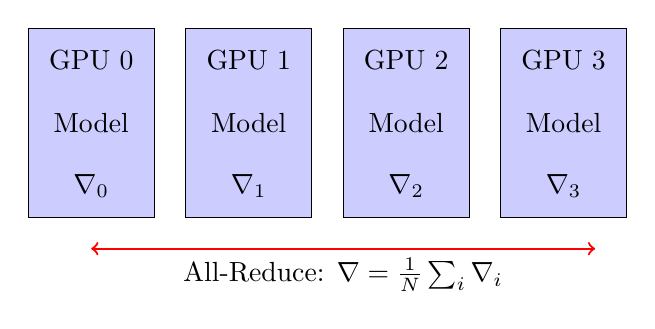
\begin{tikzpicture}[scale=0.8]
    % GPUs
    \foreach \i in {0,1,2,3} {
        \draw[fill=blue!20] (\i*2.5, 0) rectangle (\i*2.5+2, 3);
        \node at (\i*2.5+1, 2.5) {GPU \i};
        \node at (\i*2.5+1, 1.5) {Model};
        \node at (\i*2.5+1, 0.5) {$\nabla_\i$};
    }

    % All-Reduce
    \draw[<->, thick, red] (1, -0.5) -- (9, -0.5);
    \node[below] at (5, -0.5) {All-Reduce: $\nabla = \frac{1}{N}\sum_i \nabla_i$};
\end{tikzpicture}
\caption{数据并行:每个GPU持有完整模型,梯度通过All-Reduce同步}
\label{fig:data_parallel}
\end{figure}

\subsubsection{PyTorch DDP}

PyTorch的\texttt{DistributedDataParallel}(DDP)是标准的数据并行实现:
\begin{itemize}
    \item 使用NCCL后端进行高效GPU通信
    \item 梯度计算与通信重叠(Overlap)
    \item 支持梯度桶(Gradient Bucketing)优化
\end{itemize}

\textbf{局限}:每个GPU必须能容纳完整模型,无法训练超大模型。

\subsection{ZeRO:零冗余优化器}

ZeRO(Zero Redundancy Optimizer)~\citep{rajbhandari2020zero}是DeepSpeed的核心技术,通过分片消除数据并行中的内存冗余。

\subsubsection{三个阶段}

\paragraph{ZeRO-1:优化器状态分片}
将Adam的$m, v$和FP32参数副本分片到$N$个GPU:
\begin{equation}
    \text{优化器显存}: 12\Phi \to \frac{12\Phi}{N}
\end{equation}
每个GPU只更新$1/N$的参数,通过All-Gather获取完整参数。

\textbf{显存节省}:约$4\times$(相比普通DP)

\paragraph{ZeRO-2:+ 梯度分片}
梯度也按$1/N$分片,每个GPU只保留与其优化器分片对应的梯度:
\begin{equation}
    \text{梯度显存}: 2\Phi \to \frac{2\Phi}{N}
\end{equation}
使用Reduce-Scatter替代All-Reduce。

\textbf{显存节省}:约$8\times$

\paragraph{ZeRO-3:+ 参数分片}
模型参数也分片,前向/反向传播时按需All-Gather:
\begin{equation}
    \text{参数显存}: 2\Phi \to \frac{2\Phi}{N}
\end{equation}
\textbf{显存节省}:约$N\times$(线性扩展)

\begin{table}[htbp]
\centering
\caption{ZeRO各阶段显存占用对比($N$个GPU)}
\label{tab:zero_stages}
\begin{tabular}{lccc}
\toprule
阶段 & 分片内容 & 单GPU显存 & 通信量 \\
\midrule
DDP & 无 & $16\Phi$ & $2\Phi$ \\
ZeRO-1 & 优化器状态 & $4\Phi + 12\Phi/N$ & $2\Phi$ \\
ZeRO-2 & + 梯度 & $2\Phi + 14\Phi/N$ & $2\Phi$ \\
ZeRO-3 & + 参数 & $16\Phi/N$ & $3\Phi$ \\
\bottomrule
\end{tabular}
\end{table}

\subsubsection{ZeRO-Offload与ZeRO-Infinity}

\paragraph{ZeRO-Offload}
将优化器状态和计算卸载到CPU:
\begin{itemize}
    \item GPU只保留FP16参数和梯度
    \item CPU负责FP32参数更新
    \item 单GPU可训练10B+模型
\end{itemize}

\paragraph{ZeRO-Infinity}
进一步卸载到NVMe SSD:
\begin{itemize}
    \item 利用NVMe的大容量(TB级)
    \item 512 GPU可训练万亿参数模型
    \item 带宽优化:预取、分层缓存
\end{itemize}

\subsection{模型并行}

当单个模型层无法放入单GPU时,需要模型并行。

\subsubsection{张量并行(Tensor Parallelism)}

张量并行~\citep{shoeybi2019megatron}将单个层的参数矩阵切分到多个GPU。

\paragraph{MLP层的张量并行}

对于FFN层 $Y = \text{GeLU}(XW_1)W_2$:

\textbf{列切分}$W_1$(沿输出维度):
\begin{equation}
    W_1 = [W_1^{(1)}, W_1^{(2)}], \quad Y_1 = \text{GeLU}(X W_1^{(i)})
\end{equation}
每个GPU独立计算部分输出,无需通信。

\textbf{行切分}$W_2$(沿输入维度):
\begin{equation}
    W_2 = \begin{bmatrix} W_2^{(1)} \\ W_2^{(2)} \end{bmatrix}, \quad Y = \sum_i Y_1^{(i)} W_2^{(i)}
\end{equation}
需要All-Reduce求和。

\begin{figure}[htbp]
\centering
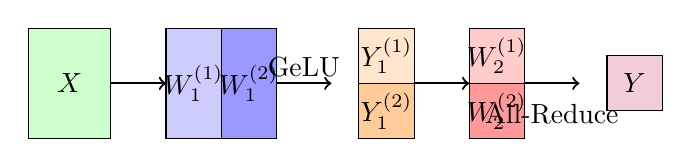
\begin{tikzpicture}[scale=0.7]
    % Input X
    \draw[fill=green!20] (0, 0) rectangle (1.5, 2);
    \node at (0.75, 1) {$X$};

    % W1 column split
    \draw[fill=blue!20] (2.5, 0) rectangle (3.5, 2);
    \draw[fill=blue!40] (3.5, 0) rectangle (4.5, 2);
    \node at (3, 1) {$W_1^{(1)}$};
    \node at (4, 1) {$W_1^{(2)}$};

    % GeLU outputs
    \draw[fill=orange!20] (6, 1) rectangle (7, 2);
    \draw[fill=orange!40] (6, 0) rectangle (7, 1);
    \node at (6.5, 1.5) {$Y_1^{(1)}$};
    \node at (6.5, 0.5) {$Y_1^{(2)}$};

    % W2 row split
    \draw[fill=red!20] (8, 1) rectangle (9, 2);
    \draw[fill=red!40] (8, 0) rectangle (9, 1);
    \node at (8.5, 1.5) {$W_2^{(1)}$};
    \node at (8.5, 0.5) {$W_2^{(2)}$};

    % Output
    \draw[fill=purple!20] (10.5, 0.5) rectangle (11.5, 1.5);
    \node at (11, 1) {$Y$};

    % Arrows
    \draw[->, thick] (1.5, 1) -- (2.5, 1);
    \draw[->, thick] (4.5, 1) -- (5.5, 1);
    \node at (5, 1.3) {GeLU};
    \draw[->, thick] (7, 1) -- (8, 1);
    \draw[->, thick] (9, 1) -- (10, 1);
    \node[below] at (9.5, 0.8) {All-Reduce};
\end{tikzpicture}
\caption{MLP层的张量并行:$W_1$列切分,$W_2$行切分}
\label{fig:tensor_parallel_mlp}
\end{figure}

\paragraph{注意力层的张量并行}

多头注意力天然适合张量并行:
\begin{itemize}
    \item 将$h$个头分配到$N$个GPU,每个GPU处理$h/N$个头
    \item $Q, K, V$投影矩阵按头切分(列切分)
    \item 输出投影$W_O$按行切分
    \item 前向需要1次All-Reduce,反向需要1次All-Reduce
\end{itemize}

\paragraph{通信开销}
每个Transformer层需要:
\begin{itemize}
    \item 前向:2次All-Reduce(注意力 + MLP)
    \item 反向:2次All-Reduce
\end{itemize}

张量并行适合\textbf{节点内}高带宽互连(NVLink: 600GB/s)。

\subsubsection{序列并行(Sequence Parallelism)}

序列并行~\citep{korthikanti2023reducing}在序列维度切分,减少激活显存:

\begin{itemize}
    \item LayerNorm和Dropout在序列维度独立,可以分片
    \item 与张量并行配合:TP区域外使用SP
    \item 将All-Reduce拆分为Reduce-Scatter + All-Gather
\end{itemize}

\textbf{优势}:激活显存降低$N$倍($N$为TP度),无额外通信。

\subsubsection{流水线并行(Pipeline Parallelism)}

流水线并行~\citep{huang2019gpipe}将模型按层切分到不同GPU:

\begin{itemize}
    \item GPU 0:Layer 0-7
    \item GPU 1:Layer 8-15
    \item ...
\end{itemize}

\paragraph{朴素流水线的问题}
顺序执行导致严重的\textbf{流水线气泡}(Pipeline Bubble):
\begin{equation}
    \text{气泡比例} = \frac{p - 1}{m + p - 1}
\end{equation}
其中$p$是流水线阶段数,$m$是micro-batch数。

\paragraph{GPipe调度}
将mini-batch切分为多个micro-batch,增大$m$减少气泡:
\begin{itemize}
    \item $m \gg p$时气泡可忽略
    \item 但需要存储所有micro-batch的激活,显存压力大
\end{itemize}

\paragraph{1F1B调度}
一个前向、一个反向交替执行:
\begin{itemize}
    \item 稳态时每个GPU同时有1个micro-batch在前向、1个在反向
    \item 激活显存只需存储$p$个micro-batch
    \item 气泡比例与GPipe相同,但显存更低
\end{itemize}

\begin{figure}[htbp]
\centering
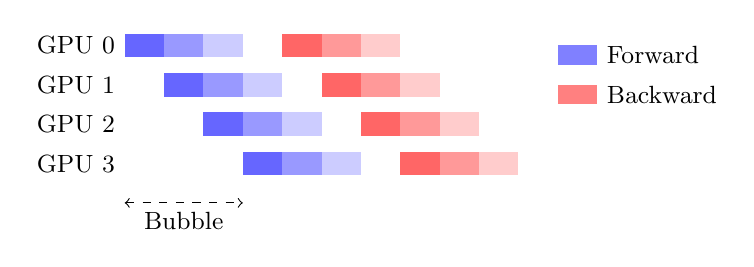
\begin{tikzpicture}[scale=0.5, font=\small]
    % Timeline labels
    \node[left] at (0, 3) {GPU 0};
    \node[left] at (0, 2) {GPU 1};
    \node[left] at (0, 1) {GPU 2};
    \node[left] at (0, 0) {GPU 3};

    % 1F1B schedule (simplified)
    % GPU 0
    \fill[blue!60] (0, 2.7) rectangle (1, 3.3);
    \fill[blue!40] (1, 2.7) rectangle (2, 3.3);
    \fill[blue!20] (2, 2.7) rectangle (3, 3.3);
    \fill[red!60] (4, 2.7) rectangle (5, 3.3);
    \fill[red!40] (5, 2.7) rectangle (6, 3.3);
    \fill[red!20] (6, 2.7) rectangle (7, 3.3);

    % GPU 1
    \fill[blue!60] (1, 1.7) rectangle (2, 2.3);
    \fill[blue!40] (2, 1.7) rectangle (3, 2.3);
    \fill[blue!20] (3, 1.7) rectangle (4, 2.3);
    \fill[red!60] (5, 1.7) rectangle (6, 2.3);
    \fill[red!40] (6, 1.7) rectangle (7, 2.3);
    \fill[red!20] (7, 1.7) rectangle (8, 2.3);

    % GPU 2
    \fill[blue!60] (2, 0.7) rectangle (3, 1.3);
    \fill[blue!40] (3, 0.7) rectangle (4, 1.3);
    \fill[blue!20] (4, 0.7) rectangle (5, 1.3);
    \fill[red!60] (6, 0.7) rectangle (7, 1.3);
    \fill[red!40] (7, 0.7) rectangle (8, 1.3);
    \fill[red!20] (8, 0.7) rectangle (9, 1.3);

    % GPU 3
    \fill[blue!60] (3, -0.3) rectangle (4, 0.3);
    \fill[blue!40] (4, -0.3) rectangle (5, 0.3);
    \fill[blue!20] (5, -0.3) rectangle (6, 0.3);
    \fill[red!60] (7, -0.3) rectangle (8, 0.3);
    \fill[red!40] (8, -0.3) rectangle (9, 0.3);
    \fill[red!20] (9, -0.3) rectangle (10, 0.3);

    % Legend
    \fill[blue!50] (11, 2.5) rectangle (12, 3);
    \node[right] at (12, 2.75) {Forward};
    \fill[red!50] (11, 1.5) rectangle (12, 2);
    \node[right] at (12, 1.75) {Backward};

    % Bubble annotation
    \draw[<->, dashed] (0, -1) -- (3, -1);
    \node[below] at (1.5, -1) {Bubble};
\end{tikzpicture}
\caption{1F1B流水线调度示意图}
\label{fig:1f1b}
\end{figure}

\subsection{3D并行}

Megatron-LM~\citep{narayanan2021efficient}将DP、TP、PP组合成\textbf{3D并行}:

\begin{equation}
    \text{总GPU数} = N_{DP} \times N_{TP} \times N_{PP}
\end{equation}

\subsubsection{并行度选择原则}

\begin{enumerate}
    \item \textbf{TP优先用于节点内}:NVLink带宽高,TP通信频繁
    \item \textbf{PP用于节点间}:通信量小(只传激活),可跨节点
    \item \textbf{DP扩展吞吐}:通信可与计算重叠
\end{enumerate}

\begin{table}[htbp]
\centering
\caption{3D并行配置示例}
\label{tab:3d_parallel}
\begin{tabular}{lccccc}
\toprule
模型 & GPU数 & TP & PP & DP & 配置说明 \\
\midrule
GPT-3 175B & 1024 & 8 & 8 & 16 & 8 GPU/节点 \\
LLaMA-70B & 64 & 8 & 2 & 4 & 单节点8卡 \\
DeepSeek-V3 & 2048 & 8 & - & 256 & MoE+EP \\
\bottomrule
\end{tabular}
\end{table}

\subsection{PyTorch FSDP}

Fully Sharded Data Parallel(FSDP)~\citep{zhao2023pytorch}是PyTorch原生的ZeRO-3实现。

\subsubsection{核心特性}

\begin{itemize}
    \item \textbf{参数分片}:模型参数、梯度、优化器状态全部分片
    \item \textbf{按需All-Gather}:前向/反向时临时恢复完整参数
    \item \textbf{Reduce-Scatter梯度}:反向后立即分片梯度
    \item \textbf{与torch.compile兼容}:可获得额外加速
\end{itemize}

\subsubsection{分片策略}

FSDP支持多种分片粒度:
\begin{itemize}
    \item \texttt{FULL\_SHARD}:完全分片(类似ZeRO-3)
    \item \texttt{SHARD\_GRAD\_OP}:只分片梯度和优化器(类似ZeRO-2)
    \item \texttt{NO\_SHARD}:不分片(类似DDP)
    \item \texttt{HYBRID\_SHARD}:节点内分片,节点间复制
\end{itemize}

\subsubsection{FSDP2}

PyTorch 2.4引入的FSDP2改进:
\begin{itemize}
    \item \textbf{Per-parameter分片}:更细粒度的控制
    \item \textbf{Selective Activation Checkpointing}:选择性重计算
    \item \textbf{SimpleFSDP}:编译器优化版本,吞吐提升可达68\%
\end{itemize}

\subsubsection{FSDP vs DeepSpeed ZeRO}

\begin{table}[htbp]
\centering
\caption{FSDP与DeepSpeed ZeRO对比}
\label{tab:fsdp_vs_zero}
\begin{tabular}{lcc}
\toprule
特性 & PyTorch FSDP & DeepSpeed ZeRO \\
\midrule
原生支持 & PyTorch内置 & 独立库 \\
CPU Offload & 支持 & 支持 \\
NVMe Offload & 有限 & ZeRO-Infinity \\
torch.compile & 兼容 & 有限 \\
配置复杂度 & 较低 & 较高 \\
生态集成 & HuggingFace等 & 广泛 \\
\bottomrule
\end{tabular}
\end{table}

\subsection{混合精度训练}

混合精度训练~\citep{micikevicius2018mixed}使用低精度(FP16/BF16)加速计算,同时保持训练稳定性。

\subsubsection{数值格式对比}

\begin{table}[htbp]
\centering
\caption{浮点数格式对比}
\label{tab:float_formats}
\begin{tabular}{lccccc}
\toprule
格式 & 位数 & 指数位 & 尾数位 & 动态范围 & 精度 \\
\midrule
FP32 & 32 & 8 & 23 & $\pm 3.4 \times 10^{38}$ & 高 \\
FP16 & 16 & 5 & 10 & $\pm 6.5 \times 10^{4}$ & 中 \\
BF16 & 16 & 8 & 7 & $\pm 3.4 \times 10^{38}$ & 低 \\
FP8 (E4M3) & 8 & 4 & 3 & $\pm 448$ & 很低 \\
FP8 (E5M2) & 8 & 5 & 2 & $\pm 5.7 \times 10^{4}$ & 极低 \\
\bottomrule
\end{tabular}
\end{table}

\subsubsection{Loss Scaling}

FP16的动态范围小,梯度可能下溢。\textbf{Loss Scaling}将损失放大:
\begin{align}
    \tilde{L} &= s \cdot L \quad \text{(放大损失)} \\
    \tilde{g} &= \nabla \tilde{L} = s \cdot \nabla L \quad \text{(放大梯度)} \\
    g &= \tilde{g} / s \quad \text{(更新前还原)}
\end{align}

\textbf{动态Loss Scaling}:
\begin{itemize}
    \item 若无溢出,增大$s$(如$s \gets 2s$)
    \item 若发生溢出(NaN/Inf),减小$s$并跳过此步更新
\end{itemize}

\subsubsection{BF16的优势}

BF16与FP32有相同的指数位,因此:
\begin{itemize}
    \item \textbf{无需Loss Scaling}:动态范围与FP32相同
    \item \textbf{训练更稳定}:不会因范围问题溢出
    \item \textbf{精度略低}:尾数只有7位(FP16有10位)
\end{itemize}

现代框架(PyTorch AMP、DeepSpeed)在支持的硬件上默认使用BF16。

\subsubsection{FP8训练}

FP8需要\textbf{每张量缩放}(Per-tensor Scaling):
\begin{itemize}
    \item 每个FP8张量有独立的缩放因子
    \item NVIDIA Transformer Engine自动管理缩放
    \item 需要torch.compile才能获得加速
    \item H100上可比BF16快约10\%
\end{itemize}

\subsection{激活检查点}

激活检查点(Activation Checkpointing)~\citep{chen2016training}通过重计算节省激活显存。

\subsubsection{原理}

前向传播时不保存中间激活,反向传播时重新计算:
\begin{itemize}
    \item \textbf{无检查点}:保存所有激活,显存$O(N)$
    \item \textbf{全检查点}:只保存输入,显存$O(1)$,计算$2\times$
    \item \textbf{$\sqrt{N}$检查点}:每$\sqrt{N}$层设检查点,显存$O(\sqrt{N})$
\end{itemize}

\subsubsection{选择性检查点}

并非所有操作都值得重计算:
\begin{itemize}
    \item \textbf{重计算}:便宜的操作(LayerNorm、激活函数、Dropout)
    \item \textbf{保存}:昂贵的操作(矩阵乘法、注意力)
\end{itemize}

PyTorch的Selective Activation Checkpointing(SAC)支持细粒度控制。

\subsubsection{注意力重计算}

注意力层的激活显存是$O(N^2)$($N$为序列长度),占比最大。FlashAttention通过:
\begin{itemize}
    \item 前向时只保存$(m, \ell)$统计量
    \item 反向时重计算注意力矩阵
\end{itemize}
实现了激活显存$O(N)$,是目前最高效的注意力重计算方案。

\subsection{集合通信}

分布式训练依赖高效的集合通信原语。

\subsubsection{常用通信原语}

\begin{table}[htbp]
\centering
\caption{集合通信原语}
\label{tab:collective_ops}
\begin{tabular}{lll}
\toprule
原语 & 功能 & 应用场景 \\
\midrule
Broadcast & 一对多广播 & 参数初始化 \\
Reduce & 多对一归约 & 梯度聚合到一个节点 \\
All-Reduce & 归约后广播 & DDP梯度同步 \\
All-Gather & 收集所有分片 & ZeRO参数恢复 \\
Reduce-Scatter & 归约后分片 & ZeRO梯度分片 \\
All-to-All & 全交换 & MoE专家通信 \\
\bottomrule
\end{tabular}
\end{table}

\subsubsection{Ring All-Reduce}

Ring All-Reduce是带宽最优的All-Reduce算法:
\begin{enumerate}
    \item \textbf{Reduce-Scatter阶段}:每个GPU向下一个发送$1/N$数据,接收并累加
    \item \textbf{All-Gather阶段}:每个GPU广播自己的归约结果
\end{enumerate}

\textbf{通信量}:$2(N-1)/N \cdot D \approx 2D$($D$为数据量),与GPU数$N$无关。

\textbf{延迟}:$O(N)$步,随GPU数线性增长(延迟非最优)。

\subsubsection{NCCL}

NVIDIA Collective Communication Library(NCCL)是GPU集群通信的标准库:
\begin{itemize}
    \item 自动选择最优拓扑(Ring、Tree、NVLink等)
    \item 支持多节点、多GPU
    \item 与CUDA深度集成
\end{itemize}

\subsection{训练框架对比}

\begin{table}[htbp]
\centering
\caption{主流训练框架对比}
\label{tab:training_frameworks}
\begin{tabular}{lccccc}
\toprule
框架 & 维护方 & TP & PP & ZeRO/FSDP & 特点 \\
\midrule
Megatron-LM & NVIDIA & \checkmark & \checkmark & ZeRO & 3D并行先驱 \\
DeepSpeed & Microsoft & \checkmark & \checkmark & ZeRO-3 & Offload、Infinity \\
PyTorch FSDP & Meta & - & - & FSDP & 原生集成 \\
Alpa & UC Berkeley & \checkmark & \checkmark & - & 自动并行 \\
ColossalAI & HPC-AI & \checkmark & \checkmark & ZeRO & 易用性 \\
\bottomrule
\end{tabular}
\end{table}

\subsection{实践建议}

\paragraph{小模型(< 10B)}
\begin{itemize}
    \item 单卡能放下:使用DDP
    \item 单卡放不下:使用FSDP或ZeRO-2
\end{itemize}

\paragraph{中等模型(10B - 100B)}
\begin{itemize}
    \item 单节点:FSDP/ZeRO-3 + 激活检查点
    \item 多节点:3D并行(TP=8节点内,PP跨节点)
\end{itemize}

\paragraph{超大模型(100B+)}
\begin{itemize}
    \item 必须使用3D并行
    \item 结合专家并行(MoE)
    \item 考虑FP8混合精度
\end{itemize}

\begin{remark}[通信与计算的权衡]
增加并行度会增加通信开销:
\begin{itemize}
    \item TP通信最频繁,应限制在高带宽节点内
    \item PP有气泡开销,需要足够的micro-batch
    \item ZeRO-3的通信量是DDP的1.5倍
\end{itemize}
最优配置需要根据具体硬件和模型进行调优。
\end{remark}


\newpage\section{Muon优化器}
\label{sec:muon}

Adam优化器自2014年提出以来,一直是深度学习的标准选择。然而,Adam本质上是\textbf{逐元素}(element-wise)的优化器,没有利用神经网络参数的\textbf{矩阵结构}。Muon(MomentUm Orthogonalized by Newton-schulz)优化器~\citep{jordan2024muon}通过对动量进行矩阵正交化,实现了更高效的参数更新,已被Kimi等大规模模型采用~\citep{liu2025muonscalable}。

\subsection{从Adam到矩阵优化}

\subsubsection{Adam的局限}

Adam的更新规则为:
\begin{align}
    m_t &= \beta_1 m_{t-1} + (1 - \beta_1) g_t \\
    v_t &= \beta_2 v_{t-1} + (1 - \beta_2) g_t^2 \\
    \theta_t &= \theta_{t-1} - \eta \cdot \frac{\hat{m}_t}{\sqrt{\hat{v}_t} + \epsilon}
\end{align}
其中所有操作都是\textbf{逐元素}进行的。对于矩阵参数$W \in \R^{d_{out} \times d_{in}}$,Adam将其展平为向量处理,完全忽略了矩阵的行列结构。

\subsubsection{矩阵参数的特殊性}

神经网络的核心参数——线性层权重矩阵——具有天然的矩阵结构:
\begin{itemize}
    \item 行向量对应输出特征的组合权重
    \item 列向量对应输入特征的映射方向
    \item 奇异值分解揭示了参数的``主方向''
\end{itemize}

一个关键观察是:SGD和Adam产生的梯度更新通常具有\textbf{极高的条件数},即接近低秩矩阵。这意味着更新主要沿少数``主方向''进行,而``稀有方向''被严重抑制。

\subsection{Muon的核心思想:正交化动量}

\subsubsection{基本算法}

Muon的核心思想是:将动量矩阵$M$替换为其最近的半正交矩阵,即进行\textbf{极分解}(Polar Decomposition)。

设$M = U\Sigma V^\top$是$M$的奇异值分解,则:
\begin{equation}
    \text{msign}(M) = UV^\top
    \label{eq:msign}
\end{equation}
这称为矩阵的\textbf{符号函数}(matrix sign function),类似于标量的sign函数将所有奇异值映射为1。

\begin{algorithm}[htbp]
\caption{Muon优化器(朴素版)}
\label{alg:muon_naive}
\begin{algorithmic}[1]
\REQUIRE 学习率$\eta$,动量系数$\beta$,初始参数$W_0$
\STATE 初始化动量 $M_0 = 0$
\FOR{$t = 1, 2, \ldots$}
    \STATE 计算梯度 $G_t = \nabla_W \mathcal{L}(W_{t-1})$
    \STATE 更新动量 $M_t = \beta M_{t-1} + G_t$
    \STATE 计算正交化更新 $\Delta_t = \text{msign}(M_t)$
    \STATE 更新参数 $W_t = W_{t-1} - \eta \cdot \Delta_t$
\ENDFOR
\end{algorithmic}
\end{algorithm}

\subsubsection{为什么正交化有效?}

要理解正交化的作用,先看Adam的问题。设梯度矩阵 $G \in \R^{d_{out} \times d_{in}}$ 的奇异值分解为 $G = U\Sigma V^\top$,其中 $\Sigma = \text{diag}(\sigma_1, \ldots, \sigma_r)$,$\sigma_1 \gg \sigma_r$(高条件数)。

\paragraph{Adam的逐元素缩放}
Adam对每个元素 $g_{ij}$ 独立归一化,这相当于在"元素坐标系"下操作。问题在于:梯度的主方向($\sigma_1$ 对应)和稀有方向($\sigma_r$ 对应)在元素坐标系中是耦合的——无法通过逐元素缩放来均衡它们。

\paragraph{Muon的谱归一化}
$\text{msign}(G) = UV^\top$ 将所有奇异值映射为1:
\begin{equation}
    G = U \cdot \text{diag}(\sigma_1, \ldots, \sigma_r) \cdot V^\top \xrightarrow{\text{msign}} U \cdot \text{diag}(1, \ldots, 1) \cdot V^\top
\end{equation}

这意味着:
\begin{enumerate}
    \item \textbf{主方向被抑制}:$\sigma_1 \to 1$,更新幅度降低
    \item \textbf{稀有方向被放大}:$\sigma_r \to 1$,更新幅度提升
    \item \textbf{方向信息保留}:$U, V$ 不变,只改变"步长"
\end{enumerate}

\paragraph{几何直觉}
想象损失函数的等高线是一个狭长的椭圆(高条件数)。Adam沿梯度方向走,容易在窄谷中震荡。Muon将椭圆"压成圆"——沿各方向走相同步长,这正是牛顿法的效果,但无需计算Hessian。

\begin{remark}[与Shampoo的关系]
Muon可以理解为"无累积的Shampoo"。Shampoo通过累积梯度的二阶统计量 $L = \sum G G^\top$,$R = \sum G^\top G$,然后用 $L^{-1/4} G R^{-1/4}$ 预条件化更新。Muon直接用当前梯度的SVD达到类似效果,避免了:
\begin{itemize}
    \item 累积带来的延迟(需要多步才能准确估计统计量)
    \item 逆矩阵平方根的高昂计算成本
    \item 大规模分布式训练中统计量同步的通信开销
\end{itemize}
代价是Muon对单步梯度的噪声更敏感,因此使用动量 $M = \beta M + G$ 来平滑。
\end{remark}

\subsection{Newton-Schulz迭代}

直接计算SVD的复杂度为$O(\min(d_{out}, d_{in})^3)$,对于大矩阵不可接受。Muon使用\textbf{Newton-Schulz迭代}高效近似$\text{msign}(M)$。

\subsubsection{迭代公式}

Newton-Schulz迭代通过多项式逼近矩阵符号函数:
\begin{equation}
    X_{k+1} = aX_k + b(X_k X_k^\top)X_k + c(X_k X_k^\top)^2 X_k
    \label{eq:newton_schulz}
\end{equation}
其中$a = 3.4445$,$b = -4.7750$,$c = 2.0315$是优化过的系数。

\subsubsection{为什么Newton-Schulz迭代有效?}

Newton-Schulz迭代的本质是用多项式逼近函数 $f(x) = \text{sign}(x) = x / |x|$。对于矩阵,这变成逐奇异值操作:$f(\sigma_i) = 1$(将所有正奇异值映射到1)。

设 $X_0 = M / \|M\|_F$(归一化使奇异值落入 $(0, 1]$),迭代后:
\begin{equation}
    X_k = U \cdot \text{diag}(\varphi^{(k)}(\sigma_1/\|M\|_F), \ldots) \cdot V^\top
\end{equation}
其中 $\varphi(x) = ax + bx^3 + cx^5$ 是设计好的五次多项式。

\paragraph{多项式设计的直觉}
目标是让 $\varphi^{(k)}(x) \to 1$ 对所有 $x \in (0, 1]$ 快速收敛。系数 $a, b, c$ 的选择使得:
\begin{itemize}
    \item $\varphi(1) = 1$(不动点)
    \item $\varphi'(1) = 0$(在不动点处导数为0,加速收敛)
    \item 对于较小的 $x$,$\varphi(x) > x$(将小值推向1)
\end{itemize}

实践中\textbf{5次迭代}即可达到足够精度。更少迭代会欠近似,更多迭代无显著收益但增加计算成本。

\subsubsection{实现代码}

\begin{lstlisting}[language=Python, caption={Newton-Schulz迭代实现}]
def newton_schulz5(G, steps=5, eps=1e-7):
    """近似计算 msign(G)"""
    a, b, c = (3.4445, -4.7750, 2.0315)
    X = G.bfloat16()
    X = X / (X.norm() + eps)  # 归一化

    # 确保 d_out <= d_in(转置处理)
    transpose = G.size(0) > G.size(1)
    if transpose:
        X = X.T

    for _ in range(steps):
        A = X @ X.T
        B = b * A + c * A @ A
        X = a * X + B @ X

    if transpose:
        X = X.T
    return X
\end{lstlisting}

\textbf{计算复杂度}:每次迭代需要$O(d_{out} \cdot d_{in} \cdot \min(d_{out}, d_{in}))$的矩阵乘法,5次迭代的总开销约为$5m/B$($m$为模型维度,$B$为batch token数),通常$< 1\%$。

\subsection{Muon的四个版本}

苏剑林在~\citep{su2025muonguide}中总结了Muon的四个主要变体,它们的唯一区别是$\text{msign}$前的\textbf{缩放因子}:

\begin{table}[htbp]
\centering
\caption{Muon四个版本的缩放因子}
\label{tab:muon_versions}
\begin{tabular}{lll}
\toprule
版本 & 缩放因子 & 特点 \\
\midrule
朴素版 & $1$ & 最简单,但学习率不可迁移 \\
KellerJordan版 & $\sqrt{\max(1, d_{out}/d_{in})}$ & 默认版本,Keras实现 \\
MuP版 & $\sqrt{d_{out}/d_{in}}$ & 学习率可迁移 \\
Moonlight版 & $0.2 \times \sqrt{\max(d_{out}, d_{in})}$ & 可直接沿用Adam学习率 \\
\bottomrule
\end{tabular}
\end{table}

\paragraph{为什么需要缩放?}
不同形状的矩阵,$\text{msign}(M)$的Frobenius范数不同(等于$\min(d_{out}, d_{in})$)。缩放因子用于:
\begin{enumerate}
    \item 使不同层的更新幅度匹配
    \item 与AdamW的更新尺度对齐
    \item 实现学习率的跨模型迁移
\end{enumerate}

\paragraph{实践建议}
\begin{itemize}
    \item \textbf{Moonlight版}:可直接沿用Adam的学习率
    \item \textbf{其他版本}:需将Adam学习率乘以约$0.2 \times \sqrt{d_{hidden}}$
\end{itemize}

\subsection{$d_{in}$和$d_{out}$的识别}

不同深度学习框架对线性层的实现方式不同,需要正确识别$d_{in}$和$d_{out}$:

\paragraph{PyTorch}
使用$y = xW^\top + b$,即$W \in \R^{d_{out} \times d_{in}}$:
\begin{lstlisting}[language=Python]
d_out, d_in = W.shape[0], W.shape[1]
\end{lstlisting}

\paragraph{Keras/TensorFlow}
使用$y = xW + b$,即$W \in \R^{d_{in} \times d_{out}}$:
\begin{lstlisting}[language=Python]
d_in, d_out = W.shape[0], W.shape[1]
\end{lstlisting}

\textbf{注意}:搞错$d_{in}$和$d_{out}$会导致缩放因子计算错误,影响训练效果。

\subsection{哪些参数使用Muon?}

Muon专为\textbf{2D矩阵参数}设计,其他参数仍需使用AdamW:

\begin{table}[htbp]
\centering
\caption{参数类型与优化器选择}
\label{tab:muon_params}
\begin{tabular}{lll}
\toprule
参数类型 & 优化器 & 原因 \\
\midrule
隐藏层Linear权重 & Muon & 核心矩阵参数 \\
Attention的$W_Q, W_K, W_V, W_O$ & Muon & 矩阵参数 \\
MLP的$W_{gate}, W_{up}, W_{down}$ & Muon & 矩阵参数 \\
\midrule
Embedding层 & AdamW & 本质是查找表 \\
最终分类头 & AdamW & 与embedding对称 \\
LayerNorm参数 & AdamW & 1D向量 \\
Bias & AdamW & 1D向量 \\
\bottomrule
\end{tabular}
\end{table}

\subsection{大规模训练:Moonlight}

月之暗面(Moonshot AI)在Moonlight模型~\citep{liu2025muonscalable}中验证了Muon的大规模可扩展性。

\subsubsection{关键技术改进}

\begin{enumerate}
    \item \textbf{添加权重衰减}:原始Muon没有weight decay,大规模训练需要加入
    \item \textbf{参数级缩放}:精确调整每个参数的更新比例(即Moonlight版的缩放因子)
\end{enumerate}

\subsubsection{分布式训练挑战}

Muon需要完整的梯度矩阵来计算正交化更新,这与现有分布式策略(ZeRO、Megatron等按元素切分优化器状态)冲突。Moonlight论文提出了内存最优、通信高效的分布式Muon实现。

\subsubsection{性能对比}

\begin{table}[htbp]
\centering
\caption{Muon vs AdamW(Moonlight实验)}
\label{tab:muon_vs_adam}
\begin{tabular}{lcc}
\toprule
指标 & Muon & AdamW \\
\midrule
计算效率 & $\sim 2\times$ & 基准 \\
达到相同性能所需FLOPs & 52\% & 100\% \\
样本效率 & 1.92$\times$ & 基准 \\
\bottomrule
\end{tabular}
\end{table}

Moonlight模型规格:
\begin{itemize}
    \item 总参数:15.29B(MoE架构)
    \item 激活参数:2.24B
    \item 训练数据:5.7T tokens
\end{itemize}

\subsection{实践指南}

\paragraph{何时使用Muon?}
\begin{itemize}
    \item 大规模预训练:Muon的效率优势随规模增大
    \item 对训练效率敏感的场景
    \item 已有AdamW超参数,想进一步优化
\end{itemize}

\paragraph{超参数设置}
\begin{itemize}
    \item \textbf{动量系数}:$\beta = 0.95$(比Adam的0.9略大)
    \item \textbf{Newton-Schulz步数}:5步
    \item \textbf{学习率}:
    \begin{itemize}
        \item Moonlight版:直接用Adam学习率
        \item 其他版本:Adam学习率 $\times$ $0.2\sqrt{d_{hidden}}$
    \end{itemize}
    \item \textbf{权重衰减}:与AdamW相同
\end{itemize}

\paragraph{注意事项}
\begin{enumerate}
    \item Muon只用于2D矩阵参数,其他参数用AdamW
    \item 正确识别框架中的$d_{in}$和$d_{out}$
    \item 对于Attention,建议对$W_Q, W_K, W_V$分别做Newton-Schulz,而非合并
    \item bfloat16精度足够,无需float32
\end{enumerate}

\begin{remark}[从向量到矩阵的本质飞跃]
苏剑林评价~\citep{su2025muonguide}:``Muon相比Adam具有更优雅的设计,体现了从向量到矩阵的本质飞跃。''Adam将矩阵展平为向量处理,而Muon真正利用了矩阵的几何结构。这种``非Element-wise''的优化范式可能代表了未来优化器的发展方向。
\end{remark}


% ============================================
% Part VI: 评测与Benchmark
% ============================================
\newpage
\part{评测与Benchmark}
\newpage\section{评测与Benchmark}
\label{sec:evaluation}

大语言模型的评测是一个复杂且快速演进的领域。本节系统介绍主流评测基准,重点关注2024年以来顶级模型(DeepSeek-V3、LLaMA 3、Qwen 2.5、GPT-4o、Claude 3.5等)普遍采用的benchmark。

\subsection{评测体系概述}

\subsubsection{为什么需要多维度评测}

单一benchmark无法全面反映模型能力:
\begin{itemize}
    \item \textbf{能力多样性}:知识、推理、代码、指令遵循等维度独立
    \item \textbf{数据污染}:训练数据可能包含测试集,导致虚高
    \item \textbf{评测饱和}:旧benchmark被刷榜,区分度下降
\end{itemize}

\subsubsection{现代评测框架}

主流模型发布时通常报告以下类别的benchmark:

\begin{table}[htbp]
\centering
\caption{评测维度与代表性Benchmark}
\label{tab:eval_dimensions}
\begin{tabular}{lll}
\toprule
维度 & 核心Benchmark & 备注 \\
\midrule
知识与理解 & MMLU, MMLU-Pro, C-Eval & 多学科知识 \\
推理能力 & GPQA, ARC-C, BBH & 复杂推理 \\
数学能力 & GSM8K, MATH-500, AIME & 从小学到竞赛 \\
代码能力 & HumanEval, LiveCodeBench & 代码生成与执行 \\
指令遵循 & IFEval, MT-Bench & 指令理解与执行 \\
长上下文 & RULER, LongBench & 长文本处理 \\
多语言 & MGSM, C-Eval & 非英语能力 \\
安全对齐 & TruthfulQA, BBQ & 真实性与偏见 \\
\bottomrule
\end{tabular}
\end{table}

\subsection{知识与理解}

\subsubsection{MMLU (Massive Multitask Language Understanding)}

MMLU是最广泛使用的知识评测基准,覆盖57个学科:
\begin{itemize}
    \item \textbf{规模}:约14,000道四选一题目
    \item \textbf{学科}:STEM、人文、社科、其他
    \item \textbf{难度}:从高中到研究生水平
\end{itemize}

\paragraph{评测方式}
\begin{itemize}
    \item Zero-shot或Few-shot(通常5-shot)
    \item 计算模型对A/B/C/D选项的概率
    \item 报告整体准确率和各学科准确率
\end{itemize}

\paragraph{当前水平}
\begin{table}[htbp]
\centering
\caption{MMLU性能对比(5-shot)}
\label{tab:mmlu_scores}
\begin{tabular}{lcc}
\toprule
模型 & MMLU & 发布时间 \\
\midrule
GPT-4o & 88.7\% & 2024.05 \\
Claude 3.5 Sonnet & 88.7\% & 2024.06 \\
DeepSeek-V3 & 88.5\% & 2024.12 \\
Qwen2.5-72B & 86.1\% & 2024.09 \\
LLaMA 3.1-405B & 88.6\% & 2024.07 \\
LLaMA 3.1-70B & 86.0\% & 2024.07 \\
\bottomrule
\end{tabular}
\end{table}

\subsubsection{MMLU-Pro}

MMLU的升级版,解决原版的问题:
\begin{itemize}
    \item \textbf{更多选项}:从4选1变为10选1,降低猜测收益
    \item \textbf{更难题目}:过滤简单题,保留需要推理的题目
    \item \textbf{减少噪声}:修正原MMLU中的错误标注
\end{itemize}

\paragraph{区分度更强}
\begin{itemize}
    \item MMLU上GPT-4与Claude差距约1\%
    \item MMLU-Pro上差距扩大到5-10\%
    \item 更能反映真实能力差异
\end{itemize}

\subsubsection{GPQA (Graduate-Level Google-Proof QA)}

针对研究生水平的专业问题:
\begin{itemize}
    \item \textbf{来源}:物理、化学、生物领域的博士生出题
    \item \textbf{特点}:问题设计为``Google-proof'',搜索引擎难以直接找到答案
    \item \textbf{难度}:领域专家准确率约65\%,非专家约30\%
\end{itemize}

GPQA-Diamond是其中最难的子集,是区分顶级模型的关键benchmark。

\begin{table}[htbp]
\centering
\caption{GPQA-Diamond性能对比}
\label{tab:gpqa_scores}
\begin{tabular}{lc}
\toprule
模型 & GPQA-Diamond \\
\midrule
DeepSeek-R1 & 71.5\% \\
o1-preview & 73.3\% \\
DeepSeek-V3 & 59.1\% \\
Claude 3.5 Sonnet & 59.4\% \\
GPT-4o & 53.6\% \\
LLaMA 3.1-405B & 51.1\% \\
Qwen2.5-72B & 49.0\% \\
\bottomrule
\end{tabular}
\end{table}

\subsection{推理能力}

\subsubsection{BBH (BIG-Bench Hard)}

BIG-Bench中最具挑战性的23个任务:
\begin{itemize}
    \item \textbf{任务类型}:逻辑推理、因果判断、算法执行等
    \item \textbf{特点}:之前模型表现接近随机
    \item \textbf{评测}:通常使用Chain-of-Thought prompting
\end{itemize}

\subsubsection{ARC (AI2 Reasoning Challenge)}

科学推理问题:
\begin{itemize}
    \item \textbf{ARC-Easy}:简单科学问题
    \item \textbf{ARC-Challenge}:需要多步推理的难题
    \item \textbf{来源}:美国3-9年级科学考试
\end{itemize}

\subsubsection{HellaSwag}

常识推理与句子补全:
\begin{itemize}
    \item 给定场景描述,选择最合理的后续
    \item 测试模型的常识理解能力
    \item 当前顶级模型准确率$>$95\%,区分度下降
\end{itemize}

\subsection{数学能力}

\subsubsection{GSM8K}

小学数学应用题:
\begin{itemize}
    \item \textbf{规模}:8,500道题目
    \item \textbf{难度}:2-8步推理
    \item \textbf{特点}:需要理解题意并进行多步计算
\end{itemize}

当前顶级模型准确率$>$95\%,已接近饱和。

\subsubsection{MATH}

竞赛级数学问题:
\begin{itemize}
    \item \textbf{来源}:AMC、AIME等数学竞赛
    \item \textbf{难度分级}:Level 1-5,Level 5最难
    \item \textbf{领域}:代数、几何、数论、概率等
\end{itemize}

\paragraph{MATH-500}
从MATH数据集中精选的500道高难度题目,是当前主流评测标准。

\begin{table}[htbp]
\centering
\caption{数学Benchmark性能对比}
\label{tab:math_scores}
\begin{tabular}{lccc}
\toprule
模型 & GSM8K & MATH-500 & AIME 2024 \\
\midrule
o1 & 96.4\% & 96.4\% & 74\% (44.6/60) \\
DeepSeek-R1 & 97.3\% & 97.3\% & 79.8\% (47.9/60) \\
DeepSeek-V3 & 91.1\% & 90.2\% & 39.2\% \\
Claude 3.5 Sonnet & 96.4\% & 78.3\% & - \\
GPT-4o & 95.8\% & 76.6\% & - \\
Qwen2.5-72B & 95.8\% & 83.1\% & - \\
\bottomrule
\end{tabular}
\end{table}

\subsubsection{AIME (American Invitational Mathematics Examination)}

美国数学邀请赛:
\begin{itemize}
    \item 15道填空题,每题答案为0-999的整数
    \item 代表高中竞赛最高水平
    \item 是区分推理模型(o1、R1)与普通模型的关键benchmark
\end{itemize}

\subsection{代码能力}

\subsubsection{HumanEval}

Python函数生成:
\begin{itemize}
    \item \textbf{规模}:164道题目
    \item \textbf{形式}:给定函数签名和docstring,生成实现
    \item \textbf{评测}:Pass@k(k次采样至少一次通过)
\end{itemize}

\paragraph{HumanEval+}
增加更多测试用例,减少假阳性。

\subsubsection{MBPP (Mostly Basic Python Problems)}

更大规模的Python编程问题:
\begin{itemize}
    \item \textbf{规模}:974道题目
    \item \textbf{难度}:相对简单,入门级编程
    \item \textbf{用途}:与HumanEval互补
\end{itemize}

\subsubsection{LiveCodeBench}

\textbf{2024年最重要的代码评测创新},解决数据污染问题:
\begin{itemize}
    \item \textbf{持续更新}:从LeetCode、AtCoder、CodeForces持续收集新题
    \item \textbf{时间标记}:每道题有发布日期,可验证是否在训练数据截止日期之后
    \item \textbf{多维度}:代码生成、自我修复、测试输出预测
\end{itemize}

\paragraph{为什么LiveCodeBench重要}
\begin{itemize}
    \item HumanEval已被``刷榜'',很多模型在训练数据中见过
    \item LiveCodeBench的新题确保公平评测
    \item 是当前评估代码能力的金标准
\end{itemize}

\subsubsection{SWE-bench}

软件工程真实任务:
\begin{itemize}
    \item \textbf{任务}:修复GitHub上真实的issue
    \item \textbf{形式}:给定代码仓库和issue描述,生成patch
    \item \textbf{难度}:需要理解大型代码库,非常具有挑战性
\end{itemize}

\begin{table}[htbp]
\centering
\caption{代码Benchmark性能对比}
\label{tab:code_scores}
\begin{tabular}{lccc}
\toprule
模型 & HumanEval & LiveCodeBench & SWE-bench Verified \\
\midrule
Claude 3.5 Sonnet & 92.0\% & 41.4\% & 50.8\% \\
DeepSeek-V3 & 82.6\% & 40.5\% & 42.0\% \\
GPT-4o & 90.2\% & 34.2\% & 38.4\% \\
o1-preview & 92.4\% & - & 41.3\% \\
Qwen2.5-72B & 86.6\% & 32.8\% & - \\
\bottomrule
\end{tabular}
\end{table}

\subsection{指令遵循}

\subsubsection{IFEval (Instruction Following Evaluation)}

测试模型严格遵循指令的能力:
\begin{itemize}
    \item \textbf{规模}:500+条带约束的指令
    \item \textbf{约束类型}:
    \begin{itemize}
        \item 长度约束:``写超过400字''
        \item 格式约束:``用JSON格式输出''
        \item 内容约束:``至少提到3次AI''
        \item 结构约束:``分成5个段落''
    \end{itemize}
    \item \textbf{评测}:约束是否被满足(可程序验证)
\end{itemize}

\paragraph{两种指标}
\begin{itemize}
    \item \textbf{Prompt-level}:整个prompt的所有约束都满足
    \item \textbf{Instruction-level}:单个约束的满足率
\end{itemize}

IFEval是Open LLM Leaderboard的核心benchmark之一。

\subsubsection{MT-Bench}

多轮对话评测:
\begin{itemize}
    \item \textbf{形式}:80个两轮对话
    \item \textbf{评分}:GPT-4作为评判,1-10分
    \item \textbf{类别}:写作、角色扮演、推理、数学等8类
\end{itemize}

\subsubsection{AlpacaEval}

单轮指令跟随:
\begin{itemize}
    \item 与GPT-4的输出进行比较
    \item 报告Win Rate(胜率)
    \item AlpacaEval 2.0使用更严格的评判标准
\end{itemize}

\subsubsection{Arena-Hard}

基于Chatbot Arena的困难子集:
\begin{itemize}
    \item 从真实用户对话中筛选的500道困难问题
    \item GPT-4-Turbo作为评判
    \item 与Chatbot Arena排名高度相关
\end{itemize}

\subsection{长上下文评测}

\subsubsection{RULER}

长上下文能力的系统评测:
\begin{itemize}
    \item \textbf{任务类型}:
    \begin{itemize}
        \item Needle-in-a-Haystack:在长文本中找到特定信息
        \item Multi-hop QA:需要整合多处信息
        \item Aggregation:统计或汇总信息
    \end{itemize}
    \item \textbf{长度范围}:4K到128K+
    \item \textbf{评测}:不同长度下的准确率衰减曲线
\end{itemize}

\subsubsection{LongBench}

多任务长文本评测:
\begin{itemize}
    \item 6大类21个任务
    \item 平均长度约15K tokens
    \item 涵盖单文档/多文档QA、摘要、代码补全等
\end{itemize}

\subsubsection{Needle-in-a-Haystack}

最简单但直观的长上下文测试:
\begin{itemize}
    \item 在长文本的随机位置插入一个``针''(关键信息)
    \item 测试模型能否准确检索
    \item 生成位置-长度的热力图
\end{itemize}

\subsection{多语言评测}

\subsubsection{C-Eval / CMMLU}

中文知识评测:
\begin{itemize}
    \item \textbf{C-Eval}:52个学科,覆盖中国教育体系
    \item \textbf{CMMLU}:中文版MMLU
    \item 是评估中文能力的核心benchmark
\end{itemize}

\subsubsection{MGSM (Multilingual GSM)}

多语言数学推理:
\begin{itemize}
    \item GSM8K翻译成10种语言
    \item 测试非英语数学推理能力
    \item 揭示模型的语言偏差
\end{itemize}

\subsection{安全与对齐}

\subsubsection{TruthfulQA}

测试模型是否会生成虚假但常见的错误信息:
\begin{itemize}
    \item 817个问题,涵盖常见误解
    \item 人类因为偏见经常答错的问题
    \item 测试模型是否学习了人类的错误信念
\end{itemize}

\subsubsection{SimpleQA}

事实准确性评测(OpenAI 2024发布):
\begin{itemize}
    \item 简单的事实性问题
    \item 测试模型是否会``幻觉''错误信息
    \item 评估拒绝回答(``我不知道'')的能力
\end{itemize}

\subsection{综合评测平台}

\subsubsection{Open LLM Leaderboard}

Hugging Face维护的开放评测平台:
\begin{itemize}
    \item \textbf{当前版本(v2)包含}:
    \begin{itemize}
        \item IFEval(指令遵循)
        \item BBH(复杂推理)
        \item MATH Level 5(高难度数学)
        \item GPQA(研究生水平QA)
        \item MuSR(多步推理)
        \item MMLU-Pro(知识理解)
    \end{itemize}
    \item 任何人可以提交模型评测
    \item 透明、可复现
\end{itemize}

\subsubsection{Chatbot Arena}

基于真实用户投票的评测:
\begin{itemize}
    \item 用户盲评两个模型的回复
    \item 使用ELO排名系统
    \item 被认为是最能反映真实用户偏好的评测
    \item 但难以控制变量,不够``科学''
\end{itemize}

\subsubsection{LiveBench}

抗污染的动态评测:
\begin{itemize}
    \item 每月更新题目
    \item 严格的时间控制防止数据污染
    \item 涵盖数学、代码、推理、语言等多个维度
\end{itemize}

\subsection{评测最佳实践}

\subsubsection{避免数据污染}

\begin{itemize}
    \item \textbf{使用新benchmark}:LiveCodeBench、LiveBench等持续更新
    \item \textbf{时间切分}:确保评测数据晚于训练数据截止日期
    \item \textbf{多源验证}:同一能力用多个benchmark交叉验证
\end{itemize}

\subsubsection{评测配置标准化}

\begin{itemize}
    \item 明确报告Few-shot数量
    \item 统一prompt模板
    \item 使用相同的解码参数(temperature、top\_p等)
\end{itemize}

\subsubsection{选择合适的Benchmark}

\begin{table}[htbp]
\centering
\caption{评测场景与推荐Benchmark}
\label{tab:eval_recommendations}
\begin{tabular}{ll}
\toprule
评测目标 & 推荐Benchmark \\
\midrule
通用能力快速评估 & MMLU-Pro, GPQA-Diamond \\
数学推理 & MATH-500, AIME \\
代码生成 & LiveCodeBench, SWE-bench \\
指令遵循 & IFEval \\
长上下文 & RULER, Needle-in-Haystack \\
中文能力 & C-Eval, CMMLU \\
真实用户偏好 & Chatbot Arena, Arena-Hard \\
安全性 & TruthfulQA, SimpleQA \\
\bottomrule
\end{tabular}
\end{table}

\begin{remark}[评测的局限性]
\begin{itemize}
    \item \textbf{Benchmark ≠ 真实能力}:高分不代表实际应用效果好
    \item \textbf{优化目标错位}:过度优化benchmark可能损害通用能力
    \item \textbf{评测演进}:benchmark会饱和,需要持续更新
    \item \textbf{人类评估}:某些能力(创意、共情)难以自动评测
\end{itemize}
\end{remark}


% ============================================
% Part VII: 部署优化
% ============================================
\newpage
\part{部署优化}
\newpage\section{模型量化}
\label{sec:quantization}

模型量化是将神经网络中的浮点数表示转换为低精度表示的技术,是大语言模型高效部署的核心技术之一。本节从基础理论到LLM专用方法,系统介绍量化技术。

\subsection{量化基础}

\subsubsection{为什么需要量化}

现代LLM的参数规模带来严峻的部署挑战:
\begin{itemize}
    \item \textbf{内存需求}:70B参数模型以FP16存储需要140GB显存
    \item \textbf{带宽瓶颈}:推理时主要受限于内存带宽而非计算
    \item \textbf{能耗成本}:数据移动消耗的能量远超计算本身
\end{itemize}

量化通过降低数值精度来解决这些问题:
\begin{table}[htbp]
\centering
\caption{不同精度的存储与计算特性}
\label{tab:precision_comparison}
\begin{tabular}{lccc}
\toprule
精度 & 位宽 & 相对内存 & 典型用途 \\
\midrule
FP32 & 32 & 1$\times$ & 训练梯度累积 \\
FP16/BF16 & 16 & 0.5$\times$ & 标准训练与推理 \\
FP8 & 8 & 0.25$\times$ & 高效训练(Hopper+) \\
INT8 & 8 & 0.25$\times$ & 量化推理 \\
INT4 & 4 & 0.125$\times$ & 激进量化推理 \\
\bottomrule
\end{tabular}
\end{table}

\subsubsection{量化的数学定义}

\textbf{均匀量化}(Uniform Quantization)是最常用的量化方式。给定浮点数$x$,量化过程为:
\begin{equation}
    Q(x) = \text{clamp}\left( \left\lfloor \frac{x}{s} \right\rceil + z, 0, 2^b - 1 \right)
\end{equation}
其中$s$是缩放因子(scale),$z$是零点(zero-point),$b$是目标位宽,$\lfloor \cdot \rceil$表示四舍五入。

\textbf{反量化}(Dequantization)恢复近似值:
\begin{equation}
    \hat{x} = s \cdot (Q(x) - z)
\end{equation}

\paragraph{对称量化 vs 非对称量化}

\textbf{对称量化}:$z = 0$,量化范围关于零点对称:
\begin{equation}
    s = \frac{\max(|x|)}{2^{b-1} - 1}
\end{equation}

\textbf{非对称量化}:允许$z \neq 0$,更好地适应非对称分布:
\begin{align}
    s &= \frac{\max(x) - \min(x)}{2^b - 1} \\
    z &= \left\lfloor -\frac{\min(x)}{s} \right\rceil
\end{align}

对称量化实现更简单(无需存储$z$),但非对称量化对偏斜分布更有效。

\subsubsection{量化粒度}

量化参数$s, z$的计算粒度影响精度与开销的权衡:

\begin{itemize}
    \item \textbf{Per-Tensor}:整个张量共享一组$(s, z)$,开销最小但精度损失大
    \item \textbf{Per-Channel}:每个输出通道独立量化,常用于权重
    \item \textbf{Per-Token}:每个token独立量化,常用于激活值
    \item \textbf{Per-Group}:将通道分组,每组独立量化,精度与开销的折中
\end{itemize}

\begin{example}[Group Quantization]
对于权重矩阵$W \in \R^{m \times n}$,设group size为$g$,则需要存储$\lceil n/g \rceil$组量化参数。常见设置$g = 128$,在INT4量化时有效位宽约为$4 + 32/128 = 4.25$位。
\end{example}

\subsection{训练后量化(PTQ)}

训练后量化(Post-Training Quantization)在模型训练完成后进行,无需重新训练,是LLM量化的主流方法。

\subsubsection{基本PTQ流程}

\begin{enumerate}
    \item \textbf{校准}(Calibration):使用少量代表性数据(通常几百到几千样本)统计激活值分布
    \item \textbf{确定量化参数}:根据统计信息计算$s, z$
    \item \textbf{量化权重}:将浮点权重转换为低精度表示
    \item \textbf{(可选)校正}:通过额外优化减少量化误差
\end{enumerate}

\subsubsection{校准策略}

\paragraph{MinMax校准}
最简单的方法,使用观测到的最大最小值:
\begin{equation}
    s = \frac{\max(x) - \min(x)}{2^b - 1}
\end{equation}
问题:对离群值敏感。

\paragraph{百分位校准}
使用第$p$和$100-p$百分位数代替最大最小值,$p$通常取0.1-1\%。

\paragraph{MSE校准}
最小化量化误差:
\begin{equation}
    s^* = \arg\min_s \mathbb{E}\left[ (x - \hat{x})^2 \right]
\end{equation}

\paragraph{KL散度校准}
最小化原始分布与量化分布的KL散度,由TensorRT采用。

\subsubsection{权重量化 vs 激活量化}

\textbf{权重量化}(W-only):
\begin{itemize}
    \item 权重在推理前确定,可以离线计算量化参数
    \item 分布通常接近高斯,易于量化
    \item 常见配置:W8A16、W4A16
\end{itemize}

\textbf{激活量化}:
\begin{itemize}
    \item 激活值依赖输入,需要动态量化或校准
    \item LLM中存在大量\textbf{离群值}(outliers),极大增加量化难度
    \item 常见配置:W8A8、W4A8
\end{itemize}

\begin{figure}[htbp]
\centering
\begin{tikzpicture}[scale=0.9]
    \draw[->] (0, 0) -- (8, 0) node[right] {值};
    \draw[->] (0, 0) -- (0, 3) node[above] {频率};
    
    \draw[blue, thick, domain=1:6, smooth] plot (\x, {2.5*exp(-0.5*(\x-3.5)^2/0.8)});
    \node[blue] at (3.5, 3) {权重分布};
    
    \draw[red, thick] (0.3, 0.2) -- (0.5, 0.3) -- (1, 0.5) -- (2, 1.5) -- (3, 2) -- (4, 1.8) -- (5, 0.8) -- (6, 0.3) -- (7, 0.1) -- (7.5, 0.08);
    \draw[red, thick, dashed] (7.5, 0.08) -- (7.8, 0.15);
    \node[red] at (6.5, 1.5) {激活分布};
    \node[red] at (7.8, 0.5) {离群值};
\end{tikzpicture}
\caption{权重与激活值的典型分布对比}
\label{fig:weight_activation_dist}
\end{figure}

\subsection{量化感知训练(QAT)}

量化感知训练(Quantization-Aware Training)在训练过程中模拟量化效果,让模型学会适应低精度表示。

\subsubsection{直通估计器(STE)}

量化操作$Q(x)$是阶梯函数,梯度几乎处处为零。\textbf{直通估计器}(Straight-Through Estimator)绕过这一问题:
\begin{equation}
    \frac{\partial \mathcal{L}}{\partial x} = \frac{\partial \mathcal{L}}{\partial Q(x)}
\end{equation}
即前向传播使用量化值,反向传播直接传递梯度。

\subsubsection{伪量化}

QAT的核心是在前向传播中插入\textbf{伪量化}(Fake Quantization)操作:
\begin{equation}
    \hat{x} = s \cdot \left( \text{clamp}\left( \left\lfloor \frac{x}{s} \right\rceil, q_{min}, q_{max} \right) \right)
\end{equation}
伪量化保持浮点计算,但模拟量化的离散化效果。

\subsubsection{QAT vs PTQ}

\begin{table}[htbp]
\centering
\caption{QAT与PTQ对比}
\label{tab:qat_vs_ptq}
\begin{tabular}{lcc}
\toprule
特性 & PTQ & QAT \\
\midrule
计算成本 & 低(分钟级) & 高(需重新训练) \\
数据需求 & 少量校准数据 & 完整训练数据 \\
精度损失 & 较大(尤其低位宽) & 较小 \\
适用场景 & 快速部署、8位量化 & 极低位宽、精度敏感 \\
\bottomrule
\end{tabular}
\end{table}

对于LLM,QAT的计算成本通常不可接受,因此PTQ是主流选择。

\subsection{LLM量化的挑战与方法}

\subsubsection{激活值离群值问题}

LLM的一个关键特性是激活值中存在\textbf{离群值}(outliers):极少数通道包含数值远大于其他通道的激活值。这些离群值:
\begin{itemize}
    \item 出现在特定通道,跨token一致
    \item 数值可达正常值的100倍以上
    \item 移除这些通道会导致模型性能崩溃
\end{itemize}

标准量化方法被迫扩大量化范围以覆盖离群值,导致正常值的量化精度严重下降。

\subsubsection{SmoothQuant}

SmoothQuant~\citep{xiao2023smoothquant}是解决激活离群值问题的突破性方法,实现了LLM的W8A8量化。

\paragraph{核心思想}
将量化难度从激活``迁移''到权重。观察到离群值出现在固定通道,可以通过per-channel缩放来平滑激活:
\begin{equation}
    Y = (X \cdot \text{diag}(s)^{-1}) \cdot (\text{diag}(s) \cdot W) = \hat{X} \hat{W}
\end{equation}
其中$s$是迁移因子。$\hat{X}$的分布更均匀,更易量化;$\hat{W}$吸收了部分难度,但权重本身分布良好,影响有限。

\paragraph{迁移因子选择}
\begin{equation}
    s_j = \frac{\max(|X_j|)^\alpha}{\max(|W_j|)^{1-\alpha}}
\end{equation}
其中$\alpha \in [0, 1]$控制迁移程度。$\alpha = 0.5$对大多数模型效果良好。

\paragraph{性能}
SmoothQuant在OPT-175B上实现了INT8量化,精度损失小于0.5\%,推理速度提升1.5倍。

\subsubsection{GPTQ}

GPTQ~\citep{frantar2022gptq}是基于二阶信息的权重量化方法,可将LLM压缩至4位精度。

\paragraph{问题形式化}
逐层优化,最小化量化后的输出误差:
\begin{equation}
    \arg\min_{\hat{W}} \| WX - \hat{W}X \|_2^2
\end{equation}

\paragraph{基于Hessian的优化}
利用Optimal Brain Quantization (OBQ)的思想,但做了关键优化使其适用于LLM规模:
\begin{enumerate}
    \item 以固定顺序(而非贪心顺序)量化权重列
    \item 批量处理多列,使用高效的矩阵运算
    \item 利用Cholesky分解高效更新Hessian逆
\end{enumerate}

\paragraph{性能}
\begin{itemize}
    \item 175B参数模型可在单GPU上4小时内完成量化
    \item 3-4位量化精度损失极小(困惑度增加$<0.5$)
    \item 广泛应用于开源LLM的量化分发
\end{itemize}

\subsubsection{AWQ}

AWQ(Activation-aware Weight Quantization)~\citep{lin2024awq}基于一个关键观察:不同权重通道的重要性差异巨大。

\paragraph{核心观察}
对于矩阵乘法$Y = XW$,如果激活值$X$的某些通道数值较大,则对应权重通道的量化误差影响更大。

\paragraph{方法}
不均匀地保护重要权重通道:
\begin{equation}
    s_j = \sqrt{\frac{\max(|X_j|)}{1 + \epsilon}}
\end{equation}
通过per-channel缩放$W_j' = W_j \cdot s_j$放大重要通道,量化后再除以$s_j$恢复。

\paragraph{性能}
在4位量化下,AWQ的困惑度通常优于GPTQ,且支持更高效的实时推理。

\subsubsection{GGUF/GGML}

GGUF(GPT-Generated Unified Format)是llama.cpp项目定义的模型存储格式,广泛用于本地LLM部署。

\paragraph{特点}
\begin{itemize}
    \item 支持多种量化格式:Q4\_0, Q4\_K\_M, Q5\_K\_M, Q8\_0等
    \item ``K''表示使用k-quant方法,对重要层使用更高精度
    \item 针对CPU推理优化,支持Apple Metal、CUDA等后端
\end{itemize}

\paragraph{常用配置}
\begin{table}[htbp]
\centering
\caption{GGUF量化格式对比}
\label{tab:gguf_formats}
\begin{tabular}{lcc}
\toprule
格式 & 有效位宽 & 精度损失 \\
\midrule
Q8\_0 & 8.5 bits & 极小 \\
Q5\_K\_M & 5.5 bits & 小 \\
Q4\_K\_M & 4.8 bits & 中等 \\
Q4\_0 & 4.5 bits & 较大 \\
Q2\_K & 3.4 bits & 大 \\
\bottomrule
\end{tabular}
\end{table}

\subsection{FP8量化}

FP8是一种8位浮点格式,相比INT8保留了动态范围,成为现代GPU训练和推理的重要选择。

\subsubsection{FP8格式}

两种主要格式:
\begin{itemize}
    \item \textbf{E4M3}:4位指数、3位尾数,动态范围更大,适合前向传播
    \item \textbf{E5M2}:5位指数、2位尾数,精度更高,适合梯度
\end{itemize}

\begin{table}[htbp]
\centering
\caption{FP8格式对比}
\label{tab:fp8_formats}
\begin{tabular}{lccc}
\toprule
格式 & 动态范围 & 最大值 & 最小正数 \\
\midrule
E4M3 & $2^{15}$ & 448 & $2^{-9}$ \\
E5M2 & $2^{31}$ & 57344 & $2^{-16}$ \\
FP16 & $2^{31}$ & 65504 & $2^{-24}$ \\
\bottomrule
\end{tabular}
\end{table}

\subsubsection{FP8训练}

NVIDIA Hopper和Blackwell架构原生支持FP8 Tensor Core。DeepSeek-V3~\citep{deepseek2024v3}展示了FP8训练的工业应用:

\paragraph{混合精度策略}
\begin{itemize}
    \item 权重和激活以FP8存储和计算
    \item 累加器使用FP32保持精度
    \item 主权重副本保持FP32/BF16用于优化器更新
\end{itemize}

\paragraph{Block-wise量化}
将张量分块独立量化,每块$128 \times 128$元素共享一个缩放因子,平衡精度与开销。

\paragraph{性能收益}
\begin{itemize}
    \item 内存带宽需求减半
    \item H100上FP8吞吐量是FP16的2倍
    \item DeepSeek-V3训练仅需2.788M H800 GPU小时
\end{itemize}

\subsubsection{FP8推理}

FlashAttention-3支持FP8注意力计算:
\begin{itemize}
    \item 使用Block Quantization减少量化误差
    \item Incoherent Processing(基于Hadamard变换)进一步提升精度
    \item 接近1.2 PFLOPS的吞吐量
\end{itemize}

\subsection{极低位宽量化}

\subsubsection{INT4/W4A16}

4位权重量化是目前实用的最低位宽:
\begin{itemize}
    \item 模型大小减少4倍
    \item 推理速度提升2-4倍(受限于内存带宽)
    \item 精度损失可控(困惑度增加通常$<1$)
\end{itemize}

\paragraph{关键技术}
\begin{itemize}
    \item Group quantization(组大小128)减少误差
    \item 对敏感层(如第一层、最后一层)使用更高精度
    \item GPTQ/AWQ的二阶优化
\end{itemize}

\subsubsection{BitNet与1.58-bit量化}

BitNet 1.58~\citep{ma2024era}提出了极端量化:权重仅取$\{-1, 0, +1\}$三个值。

\paragraph{量化函数}
\begin{equation}
    W_q = \text{RoundClip}\left( \frac{W}{\gamma}, -1, 1 \right)
\end{equation}
其中$\gamma = \frac{1}{nm}\sum_{ij}|W_{ij}|$是平均绝对值。

\paragraph{计算优势}
矩阵乘法退化为加减运算,无需乘法器:
\begin{equation}
    Y = X \cdot W_q = \sum_j X_j \cdot W_{qj} = \sum_{j: W_{qj}=1} X_j - \sum_{j: W_{qj}=-1} X_j
\end{equation}

\paragraph{当前状态}
\begin{itemize}
    \item 需要从头训练,不适用于已有模型
    \item 在同等模型容量下,精度接近FP16模型
    \item 能效提升71倍(BitNet b1.58 2B4T模型)
    \item 尚未在超大规模模型上验证
\end{itemize}

\subsection{KV Cache量化}

长上下文推理的内存瓶颈主要来自KV Cache而非模型权重。KV Cache量化成为长上下文场景的关键技术。

\subsubsection{KV Cache的内存需求}

对于序列长度$L$、batch大小$B$、层数$N_L$、注意力头数$N_H$、头维度$d$:
\begin{equation}
    \text{KV Cache大小} = 2 \times B \times L \times N_L \times N_H \times d \times \text{sizeof(dtype)}
\end{equation}

以LLaMA-70B(80层、64头、128维)为例:
\begin{itemize}
    \item 100K上下文、batch=1、FP16:约40GB
    \item 同等设置使用INT4:约10GB
\end{itemize}

\subsubsection{KIVI方法}

KIVI~\citep{liu2024kivi}是KV Cache量化的代表性工作:

\paragraph{非对称量化}
Key和Value有不同的分布特性,分别使用per-channel和per-token量化:
\begin{itemize}
    \item Key:per-channel量化(通道间差异大)
    \item Value:per-token量化(token间差异大)
\end{itemize}

\paragraph{2-bit量化}
KIVI可将KV Cache压缩至2-bit,内存减少8倍,困惑度增加极小($<0.1$)。

\subsubsection{实践建议}

\begin{itemize}
    \item 中等上下文($<$32K):4-bit KV Cache足够
    \item 长上下文(32K-128K):考虑2-bit量化
    \item 超长上下文($>$128K):结合KV Cache压缩(如H2O、StreamingLLM)
\end{itemize}

\subsection{量化的系统支持}

\subsubsection{硬件支持}

不同硬件对量化精度的支持差异显著:

\begin{table}[htbp]
\centering
\caption{GPU架构的量化支持}
\label{tab:hw_quant_support}
\begin{tabular}{lccc}
\toprule
架构 & INT8 & FP8 & INT4 \\
\midrule
Ampere (A100) & Tensor Core & 无 & 软件模拟 \\
Hopper (H100) & Tensor Core & E4M3/E5M2 & 软件模拟 \\
Blackwell (B200) & Tensor Core & 增强 & FP4原生 \\
\bottomrule
\end{tabular}
\end{table}

\subsubsection{推理框架}

主流推理框架的量化支持:
\begin{itemize}
    \item \textbf{vLLM}:支持GPTQ、AWQ、FP8、SqueezeLLM
    \item \textbf{TensorRT-LLM}:INT8/INT4 weight-only、FP8、SmoothQuant
    \item \textbf{llama.cpp}:GGUF格式,支持Q2-Q8多种精度
    \item \textbf{ExLlama}:专注于4-bit量化的高效实现
\end{itemize}

\subsection{量化最佳实践}

\paragraph{精度选择}
\begin{itemize}
    \item 内存充足:FP16/BF16,无精度损失
    \item 一般部署:INT8或FP8,精度损失极小
    \item 边缘设备:INT4(GPTQ/AWQ),精度损失可接受
    \item 极限压缩:2-3 bit,需仔细评估任务影响
\end{itemize}

\paragraph{量化方法选择}
\begin{itemize}
    \item 快速部署:直接使用预量化模型(HuggingFace上大量可用)
    \item 自定义量化:AWQ通常是最佳起点
    \item 极致压缩:GPTQ可达到更低位宽
    \item 激活量化需求:SmoothQuant处理离群值
\end{itemize}

\paragraph{评估指标}
\begin{itemize}
    \item \textbf{困惑度}:最基础的质量指标
    \item \textbf{下游任务}:MMLU、GSM8K等benchmark
    \item \textbf{推理速度}:tokens/s
    \item \textbf{内存占用}:峰值显存需求
\end{itemize}

\begin{remark}[量化的trade-off]
量化不是免费的午餐。在选择量化策略时需权衡:
\begin{itemize}
    \item 精度 vs 效率:位宽越低,压缩率越高,但精度损失也越大
    \item 量化时间 vs 推理性能:复杂量化方法(如GPTQ)需要更长校准时间
    \item 通用性 vs 专用性:针对特定任务微调的模型可能需要重新量化
\end{itemize}
当前4-bit量化(GPTQ/AWQ)是精度与效率的良好平衡点,8-bit量化(INT8/FP8)则几乎无精度损失。
\end{remark}


\newpage\section{LLM推理优化}
\label{sec:inference}

LLM推理面临独特的挑战:模型参数量巨大、自回归生成逐token进行、KV Cache随序列长度增长。本章介绍主流的推理优化技术和推理引擎。

\subsection{推理基础}

\subsubsection{两阶段推理}

LLM推理分为两个阶段:

\paragraph{Prefill阶段}
处理输入prompt的所有token,生成KV Cache和第一个输出token:
\begin{itemize}
    \item \textbf{计算特性}:并行处理所有输入token,计算密集型(Compute-bound)
    \item \textbf{瓶颈}:矩阵乘法的计算量
    \item \textbf{指标}:Time To First Token(TTFT)
\end{itemize}

\paragraph{Decode阶段}
逐个生成后续token,每步只处理1个新token:
\begin{itemize}
    \item \textbf{计算特性}:自回归生成,内存带宽受限(Memory-bound)
    \item \textbf{瓶颈}:加载模型参数和KV Cache的内存带宽
    \item \textbf{指标}:Inter-Token Latency(ITL)或Tokens Per Second(TPS)
\end{itemize}

\begin{table}[htbp]
\centering
\caption{Prefill vs Decode对比}
\label{tab:prefill_decode}
\begin{tabular}{lcc}
\toprule
特性 & Prefill & Decode \\
\midrule
Token数 & $N$(输入长度) & 1 \\
计算模式 & 并行 & 串行 \\
瓶颈 & 计算 & 内存带宽 \\
GPU利用率 & 高 & 低 \\
\bottomrule
\end{tabular}
\end{table}

\subsubsection{KV Cache}

KV Cache是推理优化的核心。每个Transformer层在处理token时会生成Key和Value向量,这些向量在后续生成中被重复使用。

\paragraph{KV Cache大小}
\begin{equation}
    \text{KV Cache} = 2 \times L \times N \times h_{kv} \times d \times \text{bytes}
\end{equation}
其中$L$是层数,$N$是序列长度,$h_{kv}$是KV头数,$d$是头维度。

\textbf{示例}:LLaMA-13B,序列长度8K,BF16精度:
\begin{equation}
    2 \times 40 \times 8192 \times 40 \times 128 \times 2 = 6.7\text{GB}
\end{equation}
单个请求的KV Cache就需要6.7GB,成为主要的显存瓶颈。

\paragraph{KV Cache优化方向}
\begin{enumerate}
    \item \textbf{减少KV头数}:GQA/MQA(见第\ref{sec:mla}节)
    \item \textbf{量化}:INT8/FP8压缩KV Cache
    \item \textbf{稀疏化}:只保留重要的KV对
    \item \textbf{共享}:跨层共享KV Cache
\end{enumerate}

\subsection{批处理策略}

\subsubsection{静态批处理}

传统方法:等待凑齐一批请求后统一处理。

\textbf{问题}:
\begin{itemize}
    \item 请求长度不一,短请求需等待长请求完成
    \item 填充(Padding)浪费计算资源
    \item 吞吐量低,延迟高
\end{itemize}

\subsubsection{Continuous Batching}

Continuous Batching~\citep{yu2022orca}动态管理请求:
\begin{itemize}
    \item 请求完成后立即释放资源,新请求立即加入
    \item 无需等待整批完成
    \item 迭代级别调度,而非请求级别
\end{itemize}

\begin{figure}[htbp]
\centering
\begin{tikzpicture}[scale=0.6, font=\small]
    % Static batching
    \node[left] at (-1, 2) {\textbf{静态}};
    \fill[blue!30] (0, 1.5) rectangle (4, 2.5);
    \fill[blue!50] (0, 0.5) rectangle (6, 1.5);
    \fill[blue!70] (0, -0.5) rectangle (3, 0.5);
    \fill[gray!30] (3, -0.5) rectangle (6, 0.5);
    \fill[gray!30] (4, 1.5) rectangle (6, 2.5);
    \node at (5, 1) {Padding};

    % Continuous batching
    \node[left] at (-1, -2) {\textbf{连续}};
    \fill[blue!30] (0, -2.5) rectangle (4, -1.5);
    \fill[green!50] (4, -2.5) rectangle (7, -1.5);
    \fill[blue!50] (0, -3.5) rectangle (6, -2.5);
    \fill[blue!70] (0, -4.5) rectangle (3, -3.5);
    \fill[orange!50] (3, -4.5) rectangle (5, -3.5);
    \fill[red!50] (5, -4.5) rectangle (7, -3.5);

    % Timeline
    \draw[->, thick] (0, -5.5) -- (8, -5.5);
    \node[below] at (4, -5.5) {Time};
\end{tikzpicture}
\caption{静态批处理 vs Continuous Batching}
\label{fig:continuous_batching}
\end{figure}

\subsubsection{Chunked Prefill}

长prompt的Prefill会阻塞Decode请求。Chunked Prefill~\citep{agrawal2024sarathi}将Prefill分块:
\begin{itemize}
    \item 长Prefill拆分为多个小块
    \item 每个块与Decode请求混合执行
    \item 减少Decode请求的排队延迟
\end{itemize}

\subsubsection{Prefill-Decode分离}

DistServe~\citep{zhong2024distserve}提出将Prefill和Decode部署到不同的GPU:
\begin{itemize}
    \item \textbf{Prefill服务器}:计算密集,可用更高的张量并行度
    \item \textbf{Decode服务器}:内存密集,优化批处理大小
    \item \textbf{KV Cache传输}:通过NVLink/PCIe在服务器间传递
\end{itemize}

\textbf{优势}:
\begin{itemize}
    \item Prefill不会阻塞Decode,降低ITL
    \item 可独立扩展两种资源
    \item 针对不同阶段优化并行策略
\end{itemize}

\subsection{PagedAttention与vLLM}

vLLM~\citep{kwon2023efficient}引入PagedAttention,借鉴操作系统虚拟内存的思想管理KV Cache。

\subsubsection{传统KV Cache的问题}

传统实现预分配连续内存存储KV Cache:
\begin{itemize}
    \item 按最大序列长度预分配,造成\textbf{内存浪费}
    \item 不同请求长度不一,产生\textbf{碎片化}
    \item 无法动态扩展,限制\textbf{并发请求数}
\end{itemize}

\subsubsection{PagedAttention原理}

PagedAttention将KV Cache分成固定大小的\textbf{Page}(块):
\begin{itemize}
    \item 每个Page存储固定数量token的KV
    \item Page可以非连续存储(类似虚拟内存)
    \item 按需分配,用完即释放
\end{itemize}

\begin{figure}[htbp]
\centering
\begin{tikzpicture}[scale=0.7, font=\small]
    % Logical view
    \node at (1.5, 3) {\textbf{逻辑视图}};
    \draw[fill=blue!20] (0, 0) rectangle (3, 2.5);
    \foreach \i in {0,1,2,3,4} {
        \draw (0, \i*0.5) -- (3, \i*0.5);
        \node[left] at (0, \i*0.5+0.25) {\tiny Block \i};
    }

    % Arrow
    \draw[->, thick] (3.5, 1.25) -- (5, 1.25);
    \node[above] at (4.25, 1.25) {Page Table};

    % Physical memory
    \node at (7.5, 3) {\textbf{物理显存}};
    \draw (5.5, 0) rectangle (9.5, 2.5);
    \fill[blue!40] (5.5, 2) rectangle (6.5, 2.5);
    \fill[blue!20] (7, 1.5) rectangle (8, 2);
    \fill[blue!60] (8.5, 0.5) rectangle (9.5, 1);
    \fill[blue!30] (5.5, 0) rectangle (6.5, 0.5);
    \fill[blue!50] (7.5, 1) rectangle (8.5, 1.5);
    \node at (6, 2.25) {\tiny 0};
    \node at (7.5, 1.75) {\tiny 1};
    \node at (9, 0.75) {\tiny 2};
    \node at (6, 0.25) {\tiny 3};
    \node at (8, 1.25) {\tiny 4};
\end{tikzpicture}
\caption{PagedAttention:非连续KV Cache存储}
\label{fig:paged_attention}
\end{figure}

\subsubsection{vLLM性能}

vLLM结合PagedAttention和Continuous Batching:
\begin{itemize}
    \item 相比HuggingFace Transformers,吞吐量提升\textbf{24倍}
    \item 显存利用率接近100\%(无碎片)
    \item 支持更大的并发批处理
\end{itemize}

\subsection{Prefix Caching与SGLang}

\subsubsection{Prefix Caching动机}

许多应用场景存在\textbf{共享前缀}:
\begin{itemize}
    \item 多轮对话:System Prompt相同
    \item Few-shot学习:示例相同
    \item 批量处理:相同的指令模板
\end{itemize}

重复计算相同前缀的KV Cache造成浪费。

\subsubsection{RadixAttention}

SGLang~\citep{zheng2024sglang}提出RadixAttention,使用\textbf{基数树}(Radix Tree)管理KV Cache:
\begin{itemize}
    \item 树的每条边对应一段token序列
    \item 共享前缀的请求共享KV Cache
    \item LRU策略管理缓存淘汰
\end{itemize}

\textbf{优势}:
\begin{itemize}
    \item 自动检测和复用共享前缀
    \item 相比vLLM,吞吐量提升可达\textbf{5-6倍}
    \item 支持复杂的LLM程序(多次调用、分支)
\end{itemize}

\subsubsection{SGLang特性}

SGLang是目前最快的开源推理引擎之一:
\begin{itemize}
    \item \textbf{RadixAttention}:自动Prefix Caching
    \item \textbf{结构化输出}:压缩有限状态机加速JSON生成
    \item \textbf{投机解码}:支持EAGLE等方法
    \item \textbf{多模态}:支持Vision-Language模型
\end{itemize}

\subsection{投机解码}

投机解码(Speculative Decoding)~\citep{leviathan2023fast,chen2023accelerating}是加速自回归生成的重要技术,其核心思想是``先用小模型快速猜测,再用大模型批量验收''。

\subsubsection{核心思想与工作流程}

自回归生成的瓶颈在于每步只生成1个token,且由于大模型是Memory-bound的,输入1个token和输入$K$个token的前向时间几乎相同——计算不是瓶颈,读取权重才是。投机解码正是利用了这一特性。

\paragraph{工作流程}
\begin{enumerate}
    \item \textbf{Draft阶段}:用小模型(Draft Model)自回归生成$K$个候选token
    \item \textbf{Verify阶段}:将这$K$个token\textbf{并行}输入大模型(Target Model),一次前向得到每个位置的next token预测
    \item \textbf{Accept/Reject}:从头开始逐个比对,连续一致的token直接接受;一旦不一致,在分歧点由大模型给出正确token,后续draft token全部丢弃
    \item 重复上述过程直到生成结束
\end{enumerate}

\textbf{关键保证}:即使draft全部猜错,也能从大模型获得至少1个正确token,因此投机解码的下限就是普通自回归解码。

\subsubsection{采样场景下的验证机制}

上述流程在贪婪解码(temperature=0)下很直观:直接比较token是否相等。但在采样场景下,大模型本身的输出也是随机的,如何定义``猜对''?

设Draft模型在位置$t$生成token $x$的分布为$q(x)$,Target模型的分布为$p(x)$。投机解码需要保证\textbf{最终输出的分布严格等于$p(x)$}(无偏性),而不仅仅是加速。

\paragraph{接受概率}
对于draft生成的token $x$,以如下概率接受:
\begin{equation}
    a(x) = \min\left(1, \frac{p(x)}{q(x)}\right)
\end{equation}

直觉理解:
\begin{itemize}
    \item 若$q(x) \leq p(x)$:大模型比小模型更认可这个token,必然接受
    \item 若$q(x) > p(x)$:小模型``过于自信'',以概率$p(x)/q(x)$接受
\end{itemize}

\paragraph{拒绝后的重采样:为什么需要残差分布?}

一个自然的问题:拒绝后为什么不直接从$p(x)$采样?因为接受分支已经``预支''了部分概率质量。

\textbf{概率账本分析}:被接受分支输出token $x$的概率为:
\begin{equation}
    \Pr[\text{accept and output } x] = q(x) \cdot a(x) = \min(p(x), q(x))
\end{equation}

要使最终分布等于$p(x)$,拒绝分支必须补齐剩余的概率质量:
\begin{equation}
    p(x) - \min(p(x), q(x)) = \max(0, p(x) - q(x))
\end{equation}

因此,拒绝时从\textbf{残差分布}重采样:
\begin{equation}
    p'(x) = \frac{\max(0, p(x) - q(x))}{\sum_{x'} \max(0, p(x') - q(x'))}
\end{equation}

\paragraph{无偏性的严格证明}

记总接受概率为$\beta = \sum_x \min(p(x), q(x))$,则拒绝概率为$1-\beta$。对任意token $x$,其最终输出概率为:
\begin{align}
    \Pr[\text{output } x] &= \underbrace{\min(p(x), q(x))}_{\text{接受分支}} + \underbrace{(1-\beta) \cdot \frac{\max(0, p(x)-q(x))}{1-\beta}}_{\text{拒绝分支}} \\
    &= \min(p(x), q(x)) + \max(0, p(x)-q(x)) \\
    &= p(x) \quad \checkmark
\end{align}
最后一步利用了恒等式$\min(a,b) + \max(0, a-b) = a$。这证明了投机解码在采样场景下是\textbf{无损}的——输出分布严格等于只用Target模型逐token采样。

\paragraph{替代方案:全局上界Rejection Sampling}

经典rejection sampling的另一种做法是:先计算全局上界$M = \max_x \frac{p(x)}{q(x)}$,然后以概率$\frac{p(x)}{M \cdot q(x)}$接受。在这种方案下:
\begin{itemize}
    \item 接受分支得到的是$p/M$(缩放版的目标分布)
    \item 拒绝后可以直接从$p$重采样(因为没有``预支''问题)
    \item 但接受率为$1/M$,通常远低于残差方案的$\sum_x \min(p(x), q(x))$
\end{itemize}
残差采样之所以成为标准做法,正是因为它在保证无偏性的同时,最大化了接受率。

\begin{remark}[两token例子]
设词表$\{A, B\}$,$p(A)=0.9, p(B)=0.1$,$q(A)=0.5, q(B)=0.5$。
\begin{itemize}
    \item A的接受概率:$\min(1, 0.9/0.5)=1$,接受分支贡献$0.5$
    \item B的接受概率:$\min(1, 0.1/0.5)=0.2$,接受分支贡献$0.5 \times 0.2=0.1$
    \item 拒绝概率:$1 - 0.5 - 0.1 = 0.4$
    \item 残差分布:A剩余$0.9-0.5=0.4$,B剩余$0.1-0.1=0$,归一化后$p'(A)=1$
    \item 最终:$A = 0.5 + 0.4 \times 1 = 0.9$,$B = 0.1 + 0.4 \times 0 = 0.1$ \checkmark
\end{itemize}
若拒绝后直接从$p$采样,B会变成$0.1 + 0.4 \times 0.1 = 0.14$,分布已偏离!
\end{remark}

\paragraph{贪婪解码作为特例}

当temperature=0时,$p$和$q$退化为在argmax上概率为1的delta分布。此时验证规则简化为:
\begin{itemize}
    \item 若draft token等于Target的argmax $\Rightarrow$ 接受($p(x)=q(x)=1$)
    \item 否则 $\Rightarrow$ 拒绝并由Target给出argmax
\end{itemize}
这解释了为什么在贪婪解码下,``猜对''直观上就是``token相等''——它是采样验证机制的退化情况。

\subsubsection{加速比分析}

设Draft模型的平均接受率为$\alpha$,每次投机$K$个token:
\begin{equation}
    \text{平均接受长度} = \frac{1 - \alpha^{K+1}}{1 - \alpha}
\end{equation}

\textbf{加速比}取决于:
\begin{itemize}
    \item 接受率$\alpha$:Draft与Target越接近越好
    \item 投机长度$K$:过大会降低接受率
    \item Draft模型速度:需要比Target快很多(通常10-50倍小)
    \item 场景特点:batch较小、交互式低延迟场景收益更明显
\end{itemize}

\subsubsection{EAGLE系列:从Chain到Tree}

EAGLE~\citep{li2024eagle}是目前SOTA的投机解码方法,其核心创新是利用Target模型的\textbf{隐状态}来指导Draft生成。

\paragraph{EAGLE-1:Chain模式}

与普通Draft模型的区别在于输入:
\begin{equation}
    \text{Draft Input} = \text{Embedding}(x_t) + \text{Project}(h_t^{\text{target}})
\end{equation}
其中$h_t^{\text{target}}$是Target模型的隐状态。这使得Draft模型能够``看到''Target模型的中间表示,显著提高猜测准确率。

\textbf{Stable KV}:验证后,清除Draft模型中由自身隐状态生成的KV Cache,只保留由Target隐状态生成的部分,确保下一轮的输入分布与训练时一致。

\paragraph{EAGLE-2:Tree模式}

Chain模式每次只生成一条候选序列。Tree模式的改进是:每步生成top-$k$个候选token,形成树状结构,增加命中概率。

\begin{itemize}
    \item \textbf{Expand阶段}:每层选top-$k$,动态维护累计得分最高的路径
    \item \textbf{Select阶段}:对所有叶节点按累计得分排序,选top-$K$送入Target验证
    \item \textbf{Tree Attention}:需要特殊的attention mask,确保每个token只关注其祖先节点
\end{itemize}

\paragraph{EAGLE-3:统一训练与推理}

EAGLE-1/2的一个问题是:训练时Draft模型看到的全是Target隐状态(stable KV),但推理时大部分隐状态来自Draft自身(unstable KV)。这种train-test mismatch导致:
\begin{itemize}
    \item 第一个draft token命中率随数据量提升
    \item 第二个及之后的token命中率急剧下降(累积误差)
\end{itemize}

EAGLE-3的解决方案:
\begin{enumerate}
    \item 训练时加入unstable KV情况,统一train与test
    \item 去除隐状态监督损失,只保留next token prediction
    \item 使用多层Target隐状态(low/mid/high features)
\end{enumerate}

这些改进使EAGLE-3获得了scaling性质——更多训练数据带来持续的性能提升。

\begin{table}[htbp]
\centering
\caption{投机解码方法对比}
\label{tab:speculative_methods}
\begin{tabular}{lcccc}
\toprule
方法 & 额外模型 & 训练需求 & 加速比 & 特点 \\
\midrule
独立Draft & 是 & 无 & 2-3$\times$ & 简单通用 \\
Self-Speculative & 否 & 无 & 1.5-2$\times$ & 显存友好 \\
Medusa & 否 & 训练Head & 2-3$\times$ & 并行预测 \\
EAGLE-1 & 否 & 训练Head & 2.5-3$\times$ & Chain + 隐状态 \\
EAGLE-2 & 否 & 训练Head & 3-4$\times$ & Tree扩展 \\
EAGLE-3 & 否 & 训练Head & 4-5$\times$ & 统一train/test \\
\bottomrule
\end{tabular}
\end{table}

\subsubsection{工业应用现状}

投机解码已成为主流推理引擎的标配优化:
\begin{itemize}
    \item \textbf{Google}:官方博客明确提到speculative decoding用于加速生成,``used across Google products''
    \item \textbf{NVIDIA TensorRT-LLM}:完整支持speculative sampling,特定配置下可达3.6$\times$吞吐提升
    \item \textbf{vLLM/SGLang}:支持draft model和n-gram等多种proposal方式
    \item \textbf{OpenAI}:API提供``Predicted Outputs''功能,用户提供预测文本,模型统计accepted/rejected tokens——思路与投机解码一致,只是proposal来自用户而非draft model
\end{itemize}

\begin{remark}[适用场景]
投机解码在以下场景收益最明显:
\begin{itemize}
    \item 交互式低延迟(QPS中等、batch小):大模型逐token生成时GPU利用率低
    \item Draft与Target分布接近:验收率高才有稳定收益
    \item 生成内容可预测性强:代码补全、格式化输出等
\end{itemize}
对于大batch高吞吐场景,GPU利用率本已较高,投机解码的收益会减弱。
\end{remark}

\subsection{KV Cache压缩}

\subsubsection{KV Cache量化}

将KV Cache从FP16/BF16量化到低精度:

\paragraph{INT8/FP8量化}
vLLM、TensorRT-LLM支持的标准方法:
\begin{itemize}
    \item 显存减少50\%
    \item 精度损失很小
    \item 硬件原生支持
\end{itemize}

\paragraph{更激进的量化}
KVQuant~\citep{hooper2024kvquant}实现3-4bit量化:
\begin{itemize}
    \item Per-channel量化 + 离群值处理
    \item 支持百万级上下文(单卡A100)
    \item 1\%离群值保留可保持精度
\end{itemize}

KIVI~\citep{liu2024kivi}实现2bit量化:
\begin{itemize}
    \item Key用2bit,Value用2bit
    \item 无需训练,即插即用
    \item 显存减少约4倍
\end{itemize}

\subsubsection{KV Cache稀疏化}

并非所有KV对都同等重要,可以选择性保留。

\paragraph{H2O (Heavy-Hitter Oracle)}
动态识别重要token~\citep{zhang2024h2o}:
\begin{itemize}
    \item 基于注意力分数累积判断重要性
    \item 保留"Heavy Hitter"token
    \item 吞吐量提升40\%+
\end{itemize}

\paragraph{SnapKV}
基于观察窗口选择重要KV~\citep{li2024snapkv}:
\begin{itemize}
    \item 每个Head只关注部分位置
    \item 聚类保留关键KV
    \item 16K输入:3.6倍加速,8.2倍显存节省
\end{itemize}

\subsection{推理引擎对比}

\begin{table}[htbp]
\centering
\caption{主流LLM推理引擎对比}
\label{tab:inference_engines}
\begin{tabular}{lcccc}
\toprule
引擎 & 核心技术 & Prefix Cache & 投机解码 & 特点 \\
\midrule
vLLM & PagedAttention & 支持 & 支持 & 最广泛使用 \\
SGLang & RadixAttention & 原生 & EAGLE等 & 结构化输出快 \\
TensorRT-LLM & 深度优化 & 支持 & 多种 & NVIDIA官方 \\
llama.cpp & CPU优化 & 有限 & 支持 & 本地部署 \\
\bottomrule
\end{tabular}
\end{table}

\subsubsection{vLLM}

vLLM是目前最流行的开源推理引擎:
\begin{itemize}
    \item \textbf{PagedAttention}:高效KV Cache管理
    \item \textbf{Continuous Batching}:动态批处理
    \item \textbf{张量并行}:多GPU推理
    \item \textbf{量化}:FP8、AWQ、GPTQ
    \item \textbf{生态}:支持HuggingFace模型、OpenAI兼容API
\end{itemize}

\subsubsection{SGLang}

SGLang专注于复杂LLM应用:
\begin{itemize}
    \item \textbf{RadixAttention}:自动Prefix Caching
    \item \textbf{Frontend语言}:简化多次调用的编程
    \item \textbf{结构化输出}:JSON Schema约束生成
    \item \textbf{性能}:在某些场景比vLLM快5-6倍
\end{itemize}

\subsubsection{TensorRT-LLM}

NVIDIA官方推理库:
\begin{itemize}
    \item 深度优化的CUDA Kernel
    \item 支持Hopper特性(FP8、TMA)
    \item In-flight Batching
    \item 与Triton Inference Server集成
\end{itemize}

\subsection{推理优化最佳实践}

\paragraph{延迟优先场景}
\begin{itemize}
    \item 使用Prefix Caching(SGLang)
    \item 投机解码(EAGLE)
    \item 小批处理 + 高并行度
\end{itemize}

\paragraph{吞吐优先场景}
\begin{itemize}
    \item Continuous Batching(vLLM)
    \item 大批处理
    \item KV Cache量化
\end{itemize}

\paragraph{长上下文场景}
\begin{itemize}
    \item KV Cache量化(KVQuant、KIVI)
    \item KV Cache稀疏化(SnapKV、H2O)
    \item Prefill-Decode分离
\end{itemize}

\begin{remark}[推理优化的权衡]
没有万能方案,需要根据场景选择:
\begin{itemize}
    \item \textbf{交互式应用}:优先TTFT和ITL
    \item \textbf{批处理任务}:优先吞吐量
    \item \textbf{边缘部署}:优先显存效率
\end{itemize}
\end{remark}



% ============================================
% Part VIII: 前沿应用
% ============================================
\newpage
\part{前沿应用}
\newpage% ============================================
% 15. 多模态大模型
% ============================================
\section{多模态大模型}
\label{sec:multimodal}

随着大语言模型(LLM)在文本理解和生成上取得突破性进展,研究者开始探索如何将视觉、音频等多模态信息与语言能力相结合。多模态大模型(Multimodal Large Language Models, MLLMs)已成为人工智能领域最活跃的研究方向之一。本章将系统介绍多模态大模型的架构设计,重点讨论"原生多模态"(Native Multimodal)这一新兴范式。

\subsection{多模态大模型概述}

\subsubsection{从单模态到多模态}

传统的大语言模型只能处理文本输入和输出。为了让模型具备"看"和"听"的能力,研究者提出了多种将视觉信息融入语言模型的方法。根据模态融合的深度和方式,多模态大模型可分为以下几类:

\begin{itemize}
    \item \textbf{级联式(Cascaded)}:多个独立模型串联,如先用视觉模型提取描述,再输入语言模型
    \item \textbf{适配器式(Adapter-based)}:在预训练LLM基础上添加视觉适配器,如LLaVA、BLIP-2
    \item \textbf{原生式(Native)}:从头开始在多模态数据上联合训练,如GPT-4o、Gemini
\end{itemize}

\subsubsection{核心挑战}

构建多模态大模型面临几个关键挑战:

\textbf{模态对齐(Modality Alignment)}:图像和文本存在于不同的表示空间,需要建立有效的跨模态映射。图像是连续的像素值,而文本是离散的token序列,如何让两者在同一语义空间中对齐是核心问题。

\textbf{信息压缩}:一张224×224的图像包含50176个像素,而典型的视觉编码器会产生196-576个视觉token。如何在保留关键信息的同时压缩视觉表示,避免对LLM造成过大的序列长度负担?

\textbf{理解与生成的统一}:视觉理解(如VQA)需要高层语义抽象,而图像生成需要细粒度的像素级信息。如何在单一模型中同时支持这两种看似矛盾的需求?

\subsection{视觉编码器}

视觉编码器是多模态大模型的"眼睛",负责将图像转换为语言模型可理解的表示。

\subsubsection{Vision Transformer (ViT)}

Vision Transformer \cite{dosovitskiy2020image}将Transformer架构应用于图像处理。其核心思想是将图像切分为固定大小的patch,然后像处理文本token一样处理这些patch:

\begin{equation}
    \mathbf{z}_0 = [\mathbf{x}_\text{class}; \mathbf{E}\mathbf{x}_1; \mathbf{E}\mathbf{x}_2; ...; \mathbf{E}\mathbf{x}_N] + \mathbf{E}_\text{pos}
\end{equation}

其中$\mathbf{x}_i \in \mathbb{R}^{P^2 \cdot C}$是第$i$个图像patch的展平向量,$\mathbf{E}$是patch embedding矩阵,$\mathbf{E}_\text{pos}$是位置编码。

\subsubsection{CLIP与对比学习}

CLIP(Contrastive Language-Image Pre-training)\cite{radford2021learning}通过对比学习在4亿图像-文本对上训练视觉编码器,使其输出的图像表示与对应文本描述在语义空间中对齐:

\begin{equation}
    \mathcal{L}_\text{CLIP} = -\frac{1}{N}\sum_{i=1}^{N}\left[\log\frac{\exp(\text{sim}(\mathbf{v}_i, \mathbf{t}_i)/\tau)}{\sum_{j=1}^{N}\exp(\text{sim}(\mathbf{v}_i, \mathbf{t}_j)/\tau)}\right]
\end{equation}

CLIP的视觉编码器(通常是ViT-L/14)因其强大的跨模态对齐能力,成为早期多模态大模型的标准选择。

\subsubsection{SigLIP与改进}

SigLIP \cite{zhai2023siglip}对CLIP的训练目标进行了改进,使用sigmoid损失替代softmax:

\begin{equation}
    \mathcal{L}_\text{SigLIP} = -\frac{1}{N}\sum_{i=1}^{N}\sum_{j=1}^{N}\log\sigma(y_{ij} \cdot \text{sim}(\mathbf{v}_i, \mathbf{t}_j) \cdot \tau)
\end{equation}

其中$y_{ij} = 1$当$i=j$,否则$y_{ij} = -1$。这种设计允许更大的batch size训练,且不需要全局负样本同步,使训练更加高效。SigLIP在InternVL、Qwen2-VL等新一代模型中广泛使用。

\subsection{模态融合机制}

将视觉特征注入语言模型的方式决定了多模态模型的架构设计。目前主流的融合机制包括:

\subsubsection{线性投影(Linear Projection)}

最简单的方式是使用线性层将视觉特征映射到语言模型的embedding空间:

\begin{equation}
    \mathbf{H}_v = \mathbf{W}_\text{proj} \cdot \mathbf{Z}_\text{vision} + \mathbf{b}
\end{equation}

\textbf{LLaVA} \cite{liu2023llava}最初采用这种方法,通过一个简单的线性投影矩阵连接CLIP ViT-L/14和Vicuna:

\begin{itemize}
    \item 保持视觉编码器和LLM的参数冻结
    \item 仅训练投影矩阵(约2M参数)
    \item 两阶段训练:预训练对齐 + 指令微调
\end{itemize}

LLaVA-1.5 \cite{liu2024llava15}将线性投影升级为两层MLP,显著提升了多模态能力:

\begin{equation}
    \mathbf{H}_v = \mathbf{W}_2 \cdot \text{GELU}(\mathbf{W}_1 \cdot \mathbf{Z}_\text{vision})
\end{equation}

\subsubsection{Q-Former(Querying Transformer)}

BLIP-2 \cite{li2023blip2}提出了Q-Former架构,使用可学习的query token通过交叉注意力从视觉特征中提取信息:

\begin{equation}
    \mathbf{Q}_\text{out} = \text{CrossAttn}(\mathbf{Q}_\text{learnable}, \mathbf{K}_\text{vision}, \mathbf{V}_\text{vision})
\end{equation}

Q-Former的核心设计:
\begin{itemize}
    \item 32个可学习的query embeddings(维度768)
    \item 基于BERT初始化的Transformer块
    \item 交叉注意力层与自注意力层交替堆叠
    \item 输出固定数量的视觉token(32个),无论输入图像分辨率
\end{itemize}

\textbf{两阶段预训练}:
\begin{enumerate}
    \item 视觉-语言表示学习:使用ITC、ITM、ITG三种损失训练Q-Former与冻结的视觉编码器对齐
    \item 视觉-语言生成学习:Q-Former输出接入冻结的LLM,训练生成能力
\end{enumerate}

BLIP-2在VQAv2零样本任务上超越Flamingo-80B达8.7\%,而可训练参数仅为后者的1/54。

\subsubsection{交叉注意力适配器(Cross-Attention Adapter)}

Flamingo \cite{alayrac2022flamingo}和LLaMA 3.2 Vision采用在LLM内部插入交叉注意力层的方式:

\begin{equation}
    \mathbf{h}_l' = \mathbf{h}_l + \text{CrossAttn}(\mathbf{h}_l, \mathbf{K}_\text{vision}, \mathbf{V}_\text{vision})
\end{equation}

\textbf{Flamingo}的架构特点:
\begin{itemize}
    \item Perceiver Resampler:将可变长度的视觉特征压缩为固定长度
    \item 在LLM的每几层插入gated cross-attention层
    \item 冻结LLM参数,仅训练新增的交叉注意力层
\end{itemize}

\textbf{LLaMA 3.2 Vision} \cite{dubey2024llama3}基于LLaMA 3.1构建:
\begin{itemize}
    \item 在冻结的LLaMA 3.1文本模型上添加视觉适配器
    \item 适配器包含多层交叉注意力,将图像编码器表示注入LLM
    \item 训练过程中更新视觉编码器和适配器,但冻结LLM参数
    \item 保持文本能力不变,实现LLaMA 3.1的"即插即用"替换
\end{itemize}

\subsubsection{融合机制对比}

\begin{table}[htbp]
\centering
\caption{模态融合机制对比}
\begin{tabular}{lcccl}
\toprule
\textbf{方法} & \textbf{代表模型} & \textbf{新增参数} & \textbf{视觉token数} & \textbf{特点} \\
\midrule
线性投影 & LLaVA & $\sim$2M & 576 & 简单高效 \\
MLP投影 & LLaVA-1.5 & $\sim$20M & 576 & 表达能力更强 \\
Q-Former & BLIP-2 & $\sim$107M & 32 & 压缩视觉信息 \\
Cross-Attention & LLaMA 3.2 & $\sim$1B & 可变 & 深度融合 \\
\bottomrule
\end{tabular}
\end{table}

\subsection{代表性多模态大模型}

\subsubsection{LLaVA系列}

LLaVA(Large Language and Vision Assistant)是最具影响力的开源多模态大模型之一。

\textbf{LLaVA-1.0}:
\begin{itemize}
    \item 视觉编码器:CLIP ViT-L/14(冻结)
    \item 语言模型:Vicuna-7B/13B(冻结)
    \item 连接方式:线性投影层
    \item 训练数据:595K图像-文本对(预训练)+ 158K视觉指令数据(微调)
\end{itemize}

\textbf{LLaVA-1.5}的改进:
\begin{itemize}
    \item MLP替代线性投影
    \item 输入分辨率从224提升到336
    \item 增加学术VQA数据
    \item 更大的语言模型(Vicuna-13B)
\end{itemize}

\textbf{LLaVA-NeXT}进一步支持动态分辨率,将图像切分为多个子图像分别编码。

\subsubsection{Qwen-VL系列}

\textbf{Qwen-VL} \cite{bai2023qwenvl}使用更大的视觉编码器和更高分辨率:
\begin{itemize}
    \item 视觉编码器:OpenCLIP ViT-bigG(448×448)
    \item 语言模型:Qwen-7B
    \item 连接方式:单层交叉注意力
\end{itemize}

\textbf{Qwen2-VL} \cite{wang2024qwen2vl}的创新:
\begin{itemize}
    \item \textbf{动态分辨率}:移除ViT的绝对位置编码,引入2D-RoPE,支持任意分辨率输入
    \item \textbf{M-RoPE}:Multimodal Rotary Position Embedding,将旋转位置编码分解为时间和空间(高度、宽度)三部分,同时捕获1D文本、2D图像、3D视频的位置信息
    \item \textbf{Token压缩}:MLP层将相邻2×2 token压缩为1个,224×224图像仅产生66个视觉token
\end{itemize}

\subsubsection{InternVL系列}

InternVL \cite{chen2024internvl}的独特设计在于视觉编码器的大规模化:
\begin{itemize}
    \item 视觉编码器扩展到60亿参数(InternViT-6B)
    \item 引入QLLaMA作为"胶水层"(8B参数)连接视觉和语言
    \item 三阶段训练:对比学习 → 生成学习 → 指令微调
\end{itemize}

InternVL 2.5是首个在MMMU基准上突破70\%的开源模型,达到GPT-4o水平。

\subsection{原生多模态模型}
\label{subsec:native-multimodal}

\subsubsection{什么是"原生多模态"?}

"原生多模态"(Native Multimodal)指的是模型从设计之初就具备多模态处理能力,而非在单模态模型基础上"嫁接"其他模态。

\textbf{非原生多模态}(如ChatGPT with GPT-4V):
\begin{itemize}
    \item 文本生成:GPT-4
    \item 图像理解:GPT-4V(独立的视觉模块)
    \item 语音识别:Whisper
    \item 图像生成:DALL-E 3
    \item 各模块独立,通过API或文本中转连接
\end{itemize}

\textbf{原生多模态}(如GPT-4o、Gemini):
\begin{itemize}
    \item 单一神经网络端到端处理所有模态
    \item 在多模态数据上从头联合训练
    \item 模态间共享表示空间,实现深度融合
    \item 无需模态间的文本中转,减少信息损失
\end{itemize}

\subsubsection{GPT-4o}

GPT-4o("o"代表"omni",全能)于2024年5月发布,是OpenAI首个原生多模态旗舰模型。

\textbf{核心特点}:
\begin{itemize}
    \item 单一模型端到端处理文本、音频、视觉输入
    \item 可直接生成文本、音频、图像输出
    \item 实时语音对话延迟降至232ms(接近人类反应速度)
    \item 音频输入保留语调、情感等非语义信息
\end{itemize}

\textbf{与GPT-4V的区别}:
\begin{itemize}
    \item GPT-4V:上传图像 → 视觉模型识别 → 转换为文本描述 → GPT-4处理 → 生成回复
    \item GPT-4o:上传图像 → 直接理解并生成回复(无中间转换)
\end{itemize}

由于GPT-4o架构未公开,具体技术细节不得而知,但其性能表明原生多模态训练的巨大优势。

\subsubsection{Google Gemini}

Gemini \cite{team2023gemini}是Google的原生多模态模型系列。

\textbf{技术报告声明}:
\begin{quote}
"Gemini models are natively multimodal, as they are trained jointly across text, image, audio, and video."
\end{quote}

\textbf{架构特点}:
\begin{itemize}
    \item 早期融合(Early Fusion)架构
    \item 从预训练阶段就在多模态数据上联合训练
    \item 支持32K(Gemini 1.0)到1M(Gemini 1.5/2.5)token上下文
\end{itemize}

\textbf{模型系列}:
\begin{itemize}
    \item Gemini Ultra:最大规模,MMLU首次超越人类专家水平
    \item Gemini Pro:均衡性能与效率
    \item Gemini Nano:端侧部署优化
    \item Gemini 2.5 Pro:2025年发布,加入"思考模型"能力
\end{itemize}

\subsubsection{Meta Chameleon}

Chameleon \cite{team2024chameleon}是Meta开源的原生多模态模型,采用彻底的早期融合架构。

\textbf{核心设计}:
\begin{itemize}
    \item 将所有模态(图像、文本、代码)表示为离散token
    \item 统一的词表包含文本、代码和图像token
    \item 使用标准Transformer架构处理混合模态序列
    \item 端到端从头训练,无需单独的图像编码器/解码器
\end{itemize}

\textbf{图像离散化}:
Chameleon使用改进的VQ-VAE将图像编码为离散token:
\begin{itemize}
    \item 图像编码为1024个离散token(32×32 latent grid)
    \item Codebook大小8192
    \item 与文本token共享统一的embedding空间
\end{itemize}

\textbf{训练规模}:
\begin{itemize}
    \item 7B和34B参数版本
    \item 约4.4万亿token训练数据(文本、图像-文本对、交错序列)
    \item 超过500万A100 GPU小时
\end{itemize}

\textbf{与Gemini的区别}:
Chameleon是完全端到端的稠密模型,没有路由组件或单独的图像解码器,而Gemini使用独立的图像解码器。

\subsection{统一理解与生成}

传统多模态模型要么专注于理解(如VQA),要么专注于生成(如文生图)。近期研究开始探索在单一模型中统一这两种能力。

\subsubsection{挑战与矛盾}

理解和生成对视觉表示有不同要求:
\begin{itemize}
    \item \textbf{理解}:需要高层语义抽象,关注"是什么"
    \item \textbf{生成}:需要细粒度细节,关注"怎么画"
\end{itemize}

使用同一个视觉编码器同时服务两种任务会产生冲突——语义编码器(如CLIP)擅长理解但生成的图像缺乏细节;像素编码器(如VQ-GAN)能重建细节但语义理解能力弱。

\subsubsection{Show-o}

Show-o \cite{xie2024showo}提出用单一Transformer统一理解和生成:

\textbf{核心设计}:
\begin{itemize}
    \item \textbf{Omni-Attention}:对文本token使用因果注意力,对图像token使用全注意力
    \item \textbf{混合建模}:文本使用自回归生成,图像使用离散扩散模型
    \item \textbf{统一词表}:文本token和图像token(VQ-GAN编码)共享词表
\end{itemize}

\textbf{任务能力}:
\begin{itemize}
    \item 图像描述(Image Captioning)
    \item 视觉问答(VQA)
    \item 文本生成图像(Text-to-Image)
    \item 图像编辑(Inpainting/Outpainting)
    \item 混合模态生成
\end{itemize}

Show-o在VQAv2上超越NExT-GPT和Chameleon等更大模型,同时在图像生成上达到FID 9.24(MSCOCO 30K)。

\subsubsection{Janus}

DeepSeek的Janus \cite{wu2024janus}采用"解耦编码、统一处理"的策略:

\textbf{核心洞察}:理解和生成需要不同的视觉编码,但可以共享语言模型处理。

\textbf{双编码器设计}:
\begin{itemize}
    \item \textbf{理解编码器}:SigLIP,提取高层语义特征
    \item \textbf{生成编码器}:VQ tokenizer,产生离散视觉表示
    \item \textbf{共享Transformer}:统一处理两种编码的token序列
\end{itemize}

\textbf{Janus-Pro}(2025年1月)进一步提升:
\begin{itemize}
    \item 基于DeepSeek-LLM-7B
    \item MMBench达到79.2(超越LLaVA-v1.5)
    \item 图像生成FID 8.53(MSCOCO 30K)
\end{itemize}

\subsubsection{JanusFlow}

JanusFlow将生成端从离散token改为连续流(Rectified Flow):
\begin{itemize}
    \item 理解端保持不变(SigLIP编码器)
    \item 生成端使用Rectified Flow替代VQ tokenizer
    \item 图像生成质量进一步提升
\end{itemize}

\subsection{视觉Tokenizer}

视觉tokenizer是原生多模态和统一模型的关键组件,负责将连续图像转换为离散token。

\subsubsection{VQ-VAE与VQ-GAN}

\textbf{VQ-VAE} \cite{van2017vqvae}首次提出将连续表示映射到可学习的离散codebook:

\begin{equation}
    z_q = \arg\min_{e_k \in \mathcal{C}} \|z_e - e_k\|_2
\end{equation}

其中$z_e$是编码器输出,$\mathcal{C}$是codebook。

\textbf{VQ-GAN} \cite{esser2021vqgan}在VQ-VAE基础上引入对抗损失:

\begin{equation}
    \mathcal{L}_\text{VQ-GAN} = \mathcal{L}_\text{rec} + \mathcal{L}_\text{commit} + \mathcal{L}_\text{GAN} + \mathcal{L}_\text{perceptual}
\end{equation}

VQ-GAN能将256×256图像编码为16×16=256个离散token,每个token来自大小为1024-16384的codebook。

\subsubsection{语义vs像素Tokenizer}

\begin{table}[htbp]
\centering
\caption{视觉Tokenizer类型对比}
\begin{tabular}{lccl}
\toprule
\textbf{类型} & \textbf{代表} & \textbf{Codebook} & \textbf{特点} \\
\midrule
像素级 & VQ-GAN & 8K-16K & 重建质量高,语义弱 \\
语义级 & CLIP-ViT & - & 语义强,无法重建 \\
混合 & SEED & 8K & 兼顾语义和重建 \\
统一 & TokenFlow & 16K & 双编码器+共享映射 \\
\bottomrule
\end{tabular}
\end{table}

\subsubsection{前沿进展}

\textbf{TokenFlow}首次证明离散视觉输入可以在理解任务上超越连续编码器(如LLaVA),通过双编码器和共享映射实现语义与细节的联合优化。

\textbf{UniTok}提出统一框架,将离散视觉和语言序列用统一的next-token prediction训练,复用code embedding到MLLM token空间。

\subsection{架构演进与对比}

\subsubsection{多模态架构发展脉络}

\begin{enumerate}
    \item \textbf{2022:适配器时代}
    \begin{itemize}
        \item Flamingo:Cross-Attention + Perceiver Resampler
        \item BLIP-2:Q-Former桥接冻结编码器和LLM
    \end{itemize}

    \item \textbf{2023:简化与规模化}
    \begin{itemize}
        \item LLaVA:简单MLP投影,证明"简单也有效"
        \item Qwen-VL:更大视觉编码器(ViT-bigG)
        \item Gemini:原生多模态训练
    \end{itemize}

    \item \textbf{2024:原生与统一}
    \begin{itemize}
        \item GPT-4o:原生多模态交互
        \item Chameleon:开源早期融合
        \item Show-o/Janus:统一理解与生成
        \item LLaMA 3.2 Vision:Cross-Attention适配器
    \end{itemize}

    \item \textbf{2025:深度融合}
    \begin{itemize}
        \item InternVL 2.5:6B视觉编码器
        \item Qwen2-VL:动态分辨率 + M-RoPE
        \item Janus-Pro:更强的统一模型
    \end{itemize}
\end{enumerate}

\subsubsection{架构对比总结}

\begin{table}[htbp]
\centering
\caption{主流多模态架构对比}
\resizebox{\textwidth}{!}{
\begin{tabular}{lccccc}
\toprule
\textbf{模型} & \textbf{视觉编码器} & \textbf{融合方式} & \textbf{LLM训练} & \textbf{原生} & \textbf{统一生成} \\
\midrule
LLaVA-1.5 & CLIP ViT-L & MLP投影 & 微调 & \ding{55} & \ding{55} \\
BLIP-2 & EVA-CLIP & Q-Former & 冻结 & \ding{55} & \ding{55} \\
LLaMA 3.2 & 自定义ViT & Cross-Attn & 冻结 & \ding{55} & \ding{55} \\
Qwen2-VL & DFN ViT & MLP & 全量微调 & \ding{55} & \ding{55} \\
InternVL 2.5 & InternViT-6B & MLP & 全量微调 & \ding{55} & \ding{55} \\
\midrule
Gemini & 内置 & 早期融合 & 联合预训练 & \ding{51} & \ding{51} \\
GPT-4o & 内置 & 端到端 & 联合预训练 & \ding{51} & \ding{51} \\
Chameleon & VQ-VAE & Token统一 & 从头训练 & \ding{51} & \ding{51} \\
\midrule
Show-o & VQ-GAN & Omni-Attn & 从LLM初始化 & 部分 & \ding{51} \\
Janus & SigLIP+VQ & 解耦编码 & 从LLM初始化 & 部分 & \ding{51} \\
\bottomrule
\end{tabular}
}
\end{table}

\subsection{设计选择与权衡}

\subsubsection{视觉编码器:冻结vs微调}

\textbf{冻结}(BLIP-2, LLaMA 3.2):
\begin{itemize}
    \item 优点:保持预训练视觉能力,训练效率高
    \item 缺点:无法针对特定任务优化视觉表示
\end{itemize}

\textbf{微调}(Qwen2-VL, InternVL):
\begin{itemize}
    \item 优点:视觉表示可针对性优化
    \item 缺点:可能遗忘预训练知识,需要更多训练资源
\end{itemize}

\subsubsection{视觉Token数量}

\begin{itemize}
    \item \textbf{固定少量}(32,Q-Former):计算高效,但可能丢失细节
    \item \textbf{固定中等}(576,LLaVA):平衡信息保留和效率
    \item \textbf{动态}(Qwen2-VL):根据图像复杂度调整,最灵活
\end{itemize}

\subsubsection{原生vs适配器}

\textbf{适配器方式}的优势:
\begin{itemize}
    \item 可复用强大的预训练LLM
    \item 训练成本相对较低
    \item 保持文本能力不退化
\end{itemize}

\textbf{原生多模态}的优势:
\begin{itemize}
    \item 模态间深度融合,减少信息损失
    \item 端到端优化,无接口瓶颈
    \item 支持实时多模态交互(如语音对话)
\end{itemize}

\subsection{多模态后训练}
\label{subsec:multimodal-posttraining}

与纯文本LLM类似,多模态大模型也需要通过后训练(Post-training)来提升指令遵循能力、减少幻觉、与人类偏好对齐。然而,多模态场景引入了新的挑战:视觉-语言对齐、跨模态幻觉、以及图像条件下的偏好学习。

\subsubsection{视觉指令微调}

视觉指令微调(Visual Instruction Tuning)是多模态后训练的基础阶段,通过高质量的多模态指令数据训练模型遵循视觉相关的指令。

\textbf{LLaVA的开创性工作} \cite{liu2023llava}:
\begin{itemize}
    \item 首次使用纯文本GPT-4生成多模态指令数据
    \item 基于COCO图像和边界框/描述,扩展为三类指令:对话式QA、详细描述、复杂推理
    \item 训练数据:558K预训练对齐数据 + 665K指令微调数据
\end{itemize}

\textbf{数据质量的重要性}:
LLaVA系列的演进(1.0 → 1.5 → NeXT)充分证明了数据质量对视觉指令微调的关键作用:
\begin{itemize}
    \item \textbf{数据多样性}:覆盖对话、描述、推理、学术VQA等多种任务
    \item \textbf{数据复杂度}:从简单问答到多轮对话、长文本描述
    \item \textbf{语言多样性}:ShareGPT4V等数据集支持多语言指令
\end{itemize}

\textbf{两阶段训练范式}:
\begin{enumerate}
    \item \textbf{预训练对齐}:在大规模图像-文本对上训练投影层,建立视觉-语言连接
    \item \textbf{指令微调}:在高质量指令数据上微调,获得指令遵循能力
\end{enumerate}

\subsubsection{多模态RLHF}

将RLHF(Reinforcement Learning from Human Feedback)从文本域扩展到多模态场景,面临独特挑战。

\textbf{LLaVA-RLHF} \cite{sun2023llava-rlhf}是首个开源的多模态RLHF工作:

\textbf{核心问题}:多模态幻觉——模型生成的文本与图像内容不符。

\textbf{方法}:Factually Augmented RLHF (Fact-RLHF)
\begin{itemize}
    \item 收集10K人类偏好数据,标注者比较两个回复并指出哪个更"幻觉"
    \item 使用图像描述或多选题答案作为额外信息校准奖励信号
    \item 通过PPO算法优化策略模型
\end{itemize}

\textbf{训练流程}:
\begin{enumerate}
    \item 在LLaVA-SFT+基础上添加LoRA模块
    \item 用10K偏好数据训练奖励模型
    \item 通过PPO进行强化学习
\end{enumerate}

\textbf{效果}:
\begin{itemize}
    \item LLaVA-Bench:达到GPT-4纯文本版94\%的水平(此前最佳仅87\%)
    \item MMHal-Bench:相比基线提升60\%
\end{itemize}

\textbf{RLHF-V} \cite{yu2024rlhfv}提出更细粒度的方法:
\begin{itemize}
    \item 收集片段级(segment-level)纠正标注,而非整体比较
    \item 使用Dense DPO直接在细粒度反馈上优化
    \item 仅需1.4K偏好数据,将幻觉率降低34.8\%
\end{itemize}

\subsubsection{多模态DPO}

DPO(Direct Preference Optimization)因其简单高效,在文本LLM对齐中广泛使用。然而,直接将DPO应用于多模态场景面临独特问题。

\textbf{无条件偏好问题}(Unconditional Preference Problem):
标准DPO在多模态场景中,模型可能忽略图像条件,仅基于文本模式学习偏好。这导致:
\begin{itemize}
    \item 模型过度依赖语言先验
    \item 视觉信息未被充分利用
    \item 对齐效果不稳定
\end{itemize}

\textbf{mDPO} \cite{wang2024mdpo}(Multimodal DPO)解决方案:

\textbf{核心改进}:
\begin{enumerate}
    \item \textbf{图像偏好优化}:在优化语言偏好的同时,显式优化图像偏好,防止语言偏好被过度优先
    \item \textbf{奖励锚点}(Reward Anchor):强制chosen响应的奖励为正,避免其likelihood下降——这是相对偏好优化的固有问题
\end{enumerate}

\textbf{mDPO损失函数}:
\begin{equation}
    \mathcal{L}_\text{mDPO} = \mathcal{L}_\text{DPO} + \lambda_\text{img} \mathcal{L}_\text{img-pref} + \lambda_\text{anchor} \mathcal{L}_\text{anchor}
\end{equation}

\textbf{实验效果}:在多个benchmark上显著降低幻觉率,特别是在需要精确视觉理解的任务上。

\textbf{其他多模态DPO变体}:
\begin{itemize}
    \item \textbf{V-DPO}:Vision-Guided DPO,通过视觉引导生成负样本
    \item \textbf{SymMPO}:对称多模态偏好优化,在正负样本间建立对称学习
    \item \textbf{负样本增强}:通过随机裁剪或扩散模型编辑图像生成负样本
\end{itemize}

\subsubsection{多模态幻觉与评估}

多模态幻觉(Multimodal Hallucination)是指模型生成的内容与输入图像不符,是多模态后训练需要重点解决的问题。

\textbf{幻觉类型}:
\begin{itemize}
    \item \textbf{对象幻觉}(Object Hallucination):描述图像中不存在的物体
    \item \textbf{属性幻觉}(Attribute Hallucination):错误描述物体的颜色、大小、位置等
    \item \textbf{关系幻觉}(Relation Hallucination):错误描述物体间的空间或语义关系
    \item \textbf{遗漏幻觉}(Omission):未提及图像中的重要内容
    \item \textbf{捏造幻觉}(Fabrication):添加图像中不存在的信息
\end{itemize}

\textbf{POPE评估基准}:
Polling-based Object Probing Evaluation将幻觉检测转化为二分类问题:
\begin{itemize}
    \item 提问:"图像中是否有\texttt{<object>}?"
    \item 三种难度:Random(随机物体)、Popular(常见物体)、Adversarial(相关但不存在的物体)
    \item 评估指标:Accuracy、Precision、Recall、F1
\end{itemize}

\textbf{MMHal-Bench}:
专门评估真实场景中的幻觉,包含96个图像-问题对,覆盖8类问题×12个物体主题。

\textbf{幻觉缓解方法}:
\begin{itemize}
    \item \textbf{对比解码}(Contrastive Decoding):比较原图和扰动图的输出分布
    \item \textbf{视觉对比解码}(VCD):通过高斯噪声等方式扰动图像
    \item \textbf{鲁棒指令微调}:在训练数据中加入幻觉对比样本
    \item \textbf{自省解码}(Self-Introspective Decoding):让模型自我检查输出的一致性
\end{itemize}

\subsubsection{LLaVA-Critic:多模态自我评估}

LLaVA-Critic \cite{xiong2024llavacritic}是首个开源的多模态通用评估模型,能够评估多模态模型在各种任务上的表现。

\textbf{核心能力}:
\begin{enumerate}
    \item \textbf{LMM-as-a-Judge}:提供可靠的评估分数,性能媲美或超越GPT模型
    \item \textbf{偏好学习}:为偏好学习生成奖励信号,提升模型对齐能力
\end{enumerate}

\textbf{训练数据}:
LLaVA-Critic-113k数据集:
\begin{itemize}
    \item 46K图像,113K评估指令样本
    \item 两种评估模式:
    \begin{itemize}
        \item Pointwise Scoring:为单个回复打分
        \item Pairwise Ranking:比较两个回复的相对质量
    \end{itemize}
    \item 30种成对评估prompt模板
\end{itemize}

\textbf{自我奖励(Self-Rewarding)效果}:
使用LLaVA-Critic的反馈训练LLaVA-OV-7B/72B:
\begin{itemize}
    \item 在6个开放式多模态benchmark上持续提升
    \item 效果优于人类偏好训练的奖励模型
    \item 虽然仅使用图像训练,也能提升视频理解能力
\end{itemize}

这表明多模态模型可以通过自我评估实现"超人类反馈"的自我改进路径。

\subsubsection{后训练流程总结}

\begin{table}[htbp]
\centering
\caption{多模态后训练方法对比}
\resizebox{\textwidth}{!}{
\begin{tabular}{lcccc}
\toprule
\textbf{方法} & \textbf{数据需求} & \textbf{训练复杂度} & \textbf{主要目标} & \textbf{代表工作} \\
\midrule
视觉指令微调 & 指令数据 & 低 & 指令遵循 & LLaVA, LLaVA-1.5 \\
RLHF & 偏好数据+奖励模型 & 高 & 减少幻觉 & LLaVA-RLHF \\
DPO/mDPO & 偏好数据 & 中 & 偏好对齐 & mDPO, V-DPO \\
细粒度反馈 & 片段级标注 & 中 & 精确纠错 & RLHF-V \\
自我奖励 & 无需人类标注 & 中 & 自我改进 & LLaVA-Critic \\
\bottomrule
\end{tabular}
}
\end{table}

\textbf{典型后训练流程}:
\begin{enumerate}
    \item \textbf{预训练}:在大规模图像-文本数据上训练模态对齐
    \item \textbf{指令微调}(SFT):在高质量指令数据上训练
    \item \textbf{偏好对齐}(可选):使用RLHF、DPO或mDPO进一步对齐
    \item \textbf{自我改进}(可选):使用Critic模型进行迭代优化
\end{enumerate}

\subsection{未来方向}

\subsubsection{统一所有模态}

当前多数模型主要处理图像和文本,未来将扩展到:
\begin{itemize}
    \item 音频/语音的原生支持
    \item 视频理解与生成
    \item 3D场景理解
    \item 具身智能(Embodied AI)
\end{itemize}

\subsubsection{更高效的视觉表示}

\begin{itemize}
    \item 自适应token数量:根据图像内容复杂度动态调整
    \item 更强的压缩:在更少token中保留更多信息
    \item 层次化表示:粗粒度语义 + 细粒度细节
\end{itemize}

\subsubsection{训练效率}

原生多模态训练需要海量计算资源(Chameleon: 500万A100小时)。未来方向:
\begin{itemize}
    \item 更高效的预训练方法
    \item 模块化训练:分阶段训练不同模态
    \item 合成数据增强
\end{itemize}

\subsubsection{评估与对齐}

\begin{itemize}
    \item 更全面的多模态benchmark
    \item 跨模态对齐的理论理解
    \item 多模态幻觉(hallucination)问题
\end{itemize}


\newpage% ============================================
% 16. 推理大模型
% ============================================
\section{推理大模型}
\label{sec:reasoning}

前一章讨论的推理优化技术(KV Cache、投机解码等)都致力于同一个目标:\textbf{让模型更快地回答}。但2024年的一系列突破揭示了另一个维度:有时候,\textbf{让模型更慢地回答}反而能获得更好的结果。

这不是技术的倒退,而是对"推理"本身的重新理解。传统LLM的自回归生成是一种"快思考"——每个token的生成几乎不假思索。而人类解决复杂问题时,往往需要"慢思考":反复尝试、回溯检查、探索多条路径。推理大模型(o1、R1等)将这种慢思考机制引入LLM,用推理时的额外计算换取答案质量的提升。

\subsection{从快思考到慢思考}

\subsubsection{传统LLM的局限}

传统大语言模型采用自回归生成方式,给定输入后直接预测下一个token,这种"System 1"式的快速响应在许多任务上表现出色,但在需要复杂推理的任务上存在明显局限:

\begin{itemize}
    \item \textbf{推理深度受限}:每个token的生成只依赖前面的上下文,缺乏"回头检查"的能力
    \item \textbf{错误累积}:推理链中的早期错误会传播到后续步骤
    \item \textbf{缺乏规划}:无法预先规划解题路径,只能"边走边看"
\end{itemize}

\subsubsection{测试时计算(Test-Time Compute)}

推理大模型的核心思想是\textbf{测试时计算扩展}(Test-Time Compute Scaling):在推理阶段投入更多计算资源,换取更好的输出质量。

\textbf{Snell等人(2024)} \cite{snell2024scaling}的关键发现:
\begin{itemize}
    \item 测试时计算的扩展可以比扩展模型参数更有效
    \item 使用"计算最优"策略,测试时计算效率可提升4倍以上
    \item 在FLOPs匹配的评估中,小模型+测试时计算可超越14倍大的模型
\end{itemize}

测试时计算的主要方式:
\begin{enumerate}
    \item \textbf{搜索}:生成多个候选答案,使用验证器选择最佳
    \item \textbf{思考}:让模型"思考"更长时间,生成详细的推理过程
    \item \textbf{迭代}:多轮自我修正和优化
\end{enumerate}

\subsection{链式思考与自一致性}

\subsubsection{链式思考(Chain-of-Thought)}

链式思考(CoT)提示是推理大模型的基础技术,通过引导模型生成中间推理步骤来提升复杂任务的表现。

\textbf{基本形式}:
\begin{verbatim}
Q: Roger有5个网球,他又买了2罐网球,每罐3个。
   他现在有多少网球?
A: Roger一开始有5个球。2罐网球共有2*3=6个球。
   5+6=11。答案是11。
\end{verbatim}

\textbf{Zero-shot CoT}:仅需添加"Let's think step by step"即可激发模型的推理能力。

\subsubsection{自一致性(Self-Consistency)}

自一致性 \cite{wang2023selfconsistency}是对链式思考的重要改进,核心思想是:
\begin{itemize}
    \item 对同一问题生成多条推理路径
    \item 通过多数投票选择最一致的答案
    \item 利用"殊途同归"的直觉——正确答案应该可以通过多种方式得出
\end{itemize}

\textbf{效果提升}:
\begin{itemize}
    \item GSM8K:+17.9\%
    \item SVAMP:+11.0\%
    \item AQuA:+12.2\%
    \item StrategyQA:+6.4\%
\end{itemize}

\textbf{改进方法}:
\begin{itemize}
    \item \textbf{CISC}(Confidence-Informed SC):基于置信度加权投票,减少40\%以上的采样需求
    \item \textbf{RASC}(Reasoning-Aware SC):动态调整采样数量
    \item \textbf{LSC}(Latent SC):基于语义一致性选择,适用于长文本回答
\end{itemize}

\subsection{奖励模型与验证器}

\subsubsection{结果奖励模型(ORM)}

结果奖励模型(Outcome Reward Model)只对最终答案给出奖励信号:

\begin{equation}
    r_\text{ORM}(x, y) = \begin{cases} 1 & \text{if } y \text{ is correct} \\ 0 & \text{otherwise} \end{cases}
\end{equation}

\textbf{优点}:标注成本低,只需判断最终答案对错

\textbf{缺点}:
\begin{itemize}
    \item 信用分配困难:无法区分哪一步出错
    \item 反馈延迟:只有完成整个推理后才能获得奖励
\end{itemize}

\subsubsection{过程奖励模型(PRM)}

过程奖励模型(Process Reward Model)对推理的每一步给出奖励信号 \cite{lightman2023lets}:

\begin{equation}
    r_\text{PRM}(x, y_{1:t}) = \text{score}(y_t | x, y_{1:t-1})
\end{equation}

其中$y_t$是第$t$步推理,score通常为\{-1, 0, +1\}表示\{错误, 中性, 正确\}。

\textbf{OpenAI的实验结果}:
使用pre-RLHF GPT-4作为基础模型,PRM在MATH测试集上达到78.2\%准确率,显著优于ORM。

\textbf{PRM vs ORM对比}:

\begin{table}[htbp]
\centering
\caption{过程奖励模型与结果奖励模型对比}
\begin{tabular}{lcc}
\toprule
\textbf{特性} & \textbf{ORM} & \textbf{PRM} \\
\midrule
反馈粒度 & 整体结果 & 每步过程 \\
标注成本 & 低 & 高 \\
信用分配 & 困难 & 精确 \\
奖励黑客风险 & 低 & 较高 \\
搜索效率 & 较低 & 更高 \\
\bottomrule
\end{tabular}
\end{table}

\textbf{隐式PRM}:
最近研究发现,可以通过训练ORM然后将其作为PRM使用,获得"免费"的过程奖励,无需昂贵的步骤级标注。

\subsubsection{过程优势验证器(PAV)}

PAV(Process Advantage Verifier)\cite{setlur2024rewarding}结合了过程监督和优势估计:
\begin{itemize}
    \item 相比ORM,搜索准确率提升8\%以上
    \item 计算效率提升1.5-5倍
    \item 在线RL中样本效率提升5-6倍
\end{itemize}

\subsection{搜索与规划}

\subsubsection{Best-of-N采样}

最简单的搜索策略是生成N个候选答案,使用验证器选择最佳:

\begin{equation}
    y^* = \arg\max_{y \in \{y_1, ..., y_N\}} r(x, y)
\end{equation}

OpenAI o1在AIME 2024上的表现:
\begin{itemize}
    \item 单次采样(pass@1):74\%
    \item 64次采样+共识(consensus@64):83\%
\end{itemize}

\subsubsection{蒙特卡洛树搜索(MCTS)}

MCTS将推理过程建模为树搜索问题,每个节点是一个推理状态,边是推理步骤。

\textbf{基本流程}:
\begin{enumerate}
    \item \textbf{选择}(Selection):使用UCB公式选择有潜力的节点
    \item \textbf{扩展}(Expansion):生成新的推理步骤
    \item \textbf{模拟}(Simulation):完成推理并获得结果
    \item \textbf{回传}(Backpropagation):更新路径上所有节点的价值
\end{enumerate}

\textbf{UCB公式}:
\begin{equation}
    \text{UCB}(s, a) = Q(s, a) + c \sqrt{\frac{\ln N(s)}{N(s, a)}}
\end{equation}

\textbf{MCT Self-Refine (MCTSr)}:
结合LLM自我改进与MCTS,在奥林匹克级数学问题上取得优异表现。

\textbf{SC-MCTS*}:
使用对比解码设计可解释的奖励模型,结合推测解码加速,平均每节点速度提升51.9\%。在Blocksworld数据集上超越o1-mini 17.4\%。

\subsection{OpenAI o1}

\subsubsection{核心设计}

OpenAI o1(2024年9月发布)是首个大规模商用的推理大模型,其核心创新在于将链式思考内化为模型能力。

\textbf{关键特点}:
\begin{itemize}
    \item \textbf{推理token}(Reasoning Tokens):模型在回答前生成内部推理过程
    \item \textbf{隐藏思考}:推理token对用户不可见(但会计费)
    \item \textbf{强化学习训练}:通过大规模RL学习"如何思考"
\end{itemize}

\textbf{OpenAI官方描述}:
\begin{quote}
"Similar to how a human may think for a long time before responding to a difficult question, o1 uses a chain of thought when attempting to solve a problem. Through reinforcement learning, o1 learns to hone its chain of thought and refine the strategies it uses."
\end{quote}

\subsubsection{性能表现}

\begin{table}[htbp]
\centering
\caption{o1在主要benchmark上的表现}
\begin{tabular}{lccc}
\toprule
\textbf{Benchmark} & \textbf{GPT-4o} & \textbf{o1-preview} & \textbf{o1} \\
\midrule
AIME 2024 & 12\% & 44\% & 74\% \\
Codeforces Rating & 808 & 1673 & 1891 \\
GPQA Diamond & 50.6\% & 73.3\% & 78.0\% \\
MATH-500 & 60.3\% & 85.5\% & 94.8\% \\
\bottomrule
\end{tabular}
\end{table}

\subsubsection{扩展规律}

o1展示了两个维度的扩展规律:
\begin{enumerate}
    \item \textbf{训练时计算}:更多RL训练带来更强的推理能力
    \item \textbf{测试时计算}:更长的思考时间带来更好的答案质量
\end{enumerate}

这打开了一条新的扩展路径:不仅可以通过增加参数和训练数据来提升性能,还可以通过增加推理时的计算来提升。

\subsection{DeepSeek-R1}

\subsubsection{纯RL训练的突破}

DeepSeek-R1 \cite{deepseek2025r1}(2025年1月)是首个证明\textbf{纯强化学习可以激发推理能力}的开源模型。

\textbf{DeepSeek-R1-Zero}的关键发现:
\begin{itemize}
    \item 无需SFT,仅通过RL即可获得强大推理能力
    \item 涌现出自我反思、验证、动态策略调整等高级推理模式
    \item AIME 2024:从15.6\%提升到71.0\%(pass@1),多数投票达86.7\%
\end{itemize}

\subsubsection{GRPO算法}

DeepSeek使用Group Relative Policy Optimization(GRPO)进行强化学习训练:

\textbf{核心思想}:
\begin{itemize}
    \item 省去传统RLHF中与策略模型同等规模的Critic模型
    \item 使用组内相对分数作为基线估计
    \item 大幅降低训练成本
\end{itemize}

\textbf{GRPO优化目标}:
\begin{equation}
    \mathcal{L}_\text{GRPO} = -\mathbb{E}_{x, \{y_i\}}\left[\sum_i \frac{r(x, y_i) - \bar{r}}{\sigma_r} \log \pi_\theta(y_i|x)\right]
\end{equation}

其中$\bar{r}$是组内平均奖励,$\sigma_r$是组内奖励标准差。

\subsubsection{完整训练流程}

DeepSeek-R1的训练包含四个阶段:

\begin{enumerate}
    \item \textbf{冷启动数据}:少量高质量推理数据,解决R1-Zero的可读性问题
    \item \textbf{推理RL}:大规模RL训练,发现更好的推理模式
    \item \textbf{拒绝采样SFT}:收集RL模型的优质输出进行SFT
    \item \textbf{偏好RL}:与人类偏好对齐
\end{enumerate}

\subsubsection{涌现能力}

R1-Zero在训练过程中涌现出多种高级推理行为:
\begin{itemize}
    \item \textbf{自我反思}:"Wait, let me reconsider..."
    \item \textbf{验证}:检查中间步骤的正确性
    \item \textbf{回溯}:发现错误后退回重试
    \item \textbf{策略切换}:一种方法不行时尝试另一种
\end{itemize}

\subsection{开源推理模型}

\subsubsection{QwQ(Qwen with Questions)}

QwQ \cite{qwen2024qwq}是阿里巴巴Qwen团队发布的开源推理模型(2024年11月)。

\textbf{设计理念}:
\begin{quote}
"QwQ approaches every problem with genuine wonder and doubt. It knows that it knows nothing, and that's precisely what drives its curiosity."
\end{quote}

\textbf{技术特点}:
\begin{itemize}
    \item 32B参数,32K上下文长度
    \item 使用规则化强化学习嵌入推理能力
    \item 推理时生成长思考链
\end{itemize}

\textbf{性能表现}:
\begin{itemize}
    \item GPQA:65.2\%(研究生级科学推理)
    \item AIME 2024:50.0\%
    \item MATH-500:90.6\%
    \item LiveCodeBench:50.0\%
\end{itemize}

\textbf{已知局限}:
\begin{itemize}
    \item 可能混合语言或意外切换语言
    \item 可能陷入循环推理,产生过长输出
\end{itemize}

\subsubsection{Marco-o1}

阿里巴巴的另一个推理模型Marco-o1使用MCTS算法生成合成训练数据,结合CoT样本进行训练。

\subsection{知识蒸馏}

\subsubsection{推理能力的迁移}

DeepSeek开创性地证明了推理能力可以通过蒸馏迁移到小模型。

\textbf{蒸馏方法}:
\begin{itemize}
    \item 使用DeepSeek-R1生成800K推理样本
    \item 在小模型上进行SFT(无需额外RL)
    \item 小模型获得类似的推理能力
\end{itemize}

\subsubsection{蒸馏模型系列}

\begin{table}[htbp]
\centering
\caption{DeepSeek-R1蒸馏模型性能}
\begin{tabular}{lccc}
\toprule
\textbf{模型} & \textbf{基座} & \textbf{AIME 2024} & \textbf{MATH-500} \\
\midrule
R1-Distill-Qwen-1.5B & Qwen2.5-1.5B & 28.9\% & 83.9\% \\
R1-Distill-Qwen-7B & Qwen2.5-7B & 55.5\% & 92.8\% \\
R1-Distill-Qwen-14B & Qwen2.5-14B & 69.7\% & 93.9\% \\
R1-Distill-Qwen-32B & Qwen2.5-32B & 72.6\% & 94.3\% \\
R1-Distill-Llama-8B & Llama3.1-8B & 50.4\% & 89.1\% \\
R1-Distill-Llama-70B & Llama3.3-70B & 70.0\% & 94.5\% \\
\bottomrule
\end{tabular}
\end{table}

\textbf{关键发现}:
\begin{itemize}
    \item R1-Distill-Qwen-32B超越o1-mini
    \item 蒸馏效果优于同规模模型直接RL训练
    \item 蒸馏是获得推理能力的高效途径
\end{itemize}

\subsection{技术对比与分析}

\subsubsection{主要推理模型对比}

\begin{table}[htbp]
\centering
\caption{主流推理大模型对比}
\resizebox{\textwidth}{!}{
\begin{tabular}{lcccccc}
\toprule
\textbf{模型} & \textbf{参数} & \textbf{开源} & \textbf{训练方法} & \textbf{AIME} & \textbf{MATH} & \textbf{发布} \\
\midrule
GPT-4o & - & \ding{55} & SFT & 12\% & 60.3\% & 2024.05 \\
o1-preview & - & \ding{55} & RL & 44\% & 85.5\% & 2024.09 \\
o1 & - & \ding{55} & RL & 74\% & 94.8\% & 2024.12 \\
\midrule
QwQ-32B & 32B & \ding{51} & RL & 50\% & 90.6\% & 2024.11 \\
DeepSeek-R1 & 671B & \ding{51} & RL & 79.8\% & 97.3\% & 2025.01 \\
R1-Distill-32B & 32B & \ding{51} & 蒸馏 & 72.6\% & 94.3\% & 2025.01 \\
\bottomrule
\end{tabular}
}
\end{table}

\subsubsection{训练范式对比}

\begin{itemize}
    \item \textbf{o1}:大规模RL + 隐藏推理token + 闭源
    \item \textbf{DeepSeek-R1}:GRPO + 多阶段训练 + 完全开源
    \item \textbf{QwQ}:规则化RL + 开源权重
    \item \textbf{蒸馏模型}:SFT on推理数据 + 开源
\end{itemize}

\subsection{应用与局限}

\subsubsection{适用场景}

推理大模型特别适合:
\begin{itemize}
    \item \textbf{数学问题}:竞赛数学、定理证明
    \item \textbf{代码生成}:复杂算法、调试
    \item \textbf{科学推理}:物理、化学问题
    \item \textbf{逻辑推理}:规划、约束满足
\end{itemize}

\subsubsection{当前局限}

\begin{itemize}
    \item \textbf{延迟高}:思考时间长,不适合实时交互
    \item \textbf{成本高}:推理token消耗大量计算资源
    \item \textbf{过度思考}:简单问题也可能产生冗长推理
    \item \textbf{循环推理}:可能陷入无意义的思考循环
    \item \textbf{语言混杂}:思考过程中可能混合多种语言
\end{itemize}

\subsubsection{开放问题}

\begin{itemize}
    \item \textbf{最优思考长度}:如何确定何时停止思考?
    \item \textbf{思考可解释性}:隐藏的推理过程是否可信?
    \item \textbf{通用推理}:当前主要在数学/代码领域,如何扩展到更多领域?
    \item \textbf{效率优化}:如何在保持推理质量的同时降低计算成本?
\end{itemize}

\subsection{未来方向}

\subsubsection{计算最优策略}

根据任务难度动态调整测试时计算:
\begin{itemize}
    \item 简单问题:快速响应
    \item 困难问题:深度思考
    \item 预测难度并自动选择策略
\end{itemize}

\subsubsection{多模态推理}

将推理能力扩展到多模态:
\begin{itemize}
    \item 视觉推理:图像中的逻辑关系
    \item 视频理解:时序推理
    \item 具身智能:物理世界的规划
\end{itemize}

\subsubsection{推理与Agent}

推理大模型为AI Agent提供了更强的规划能力:
\begin{itemize}
    \item 任务分解与规划
    \item 工具使用决策
    \item 长期目标追踪
\end{itemize}

\subsubsection{效率提升}

\begin{itemize}
    \item \textbf{推测解码}:加速推理token生成
    \item \textbf{早停策略}:检测到答案收敛时提前停止
    \item \textbf{轻量化}:蒸馏更小的推理模型
    \item \textbf{稀疏激活}:仅激活与推理相关的参数
\end{itemize}



% References
\bibliographystyle{plainnat}
\bibliography{references}

\end{document}
